\chapter{Sample Selections and Systematics}
\label{chap:SelsAndSysts}

The oscillation analysis presented within this thesis rests upon the simultaneous fit of atmospheric samples at SK, and beam near and far detector samples. The sample definitions and binning are documented in \autoref{sec:SelsAndSysts_Sels_Atms}, \autoref{sec:SelsAndSysts_Sels_ND}, and \autoref{sec:SelsAndSysts_Sels_FD}, respectively. This analysis uses \quickmath{1.1531 \times 10^{21}} protons on target (POT) in FHC and \quickmath{8.336 \times 10^{20}} POT in RHC for the near detector samples corresponding to Runs \quickmath{2-9}, \quickmath{1.9664 \times 10^{21}} POT in FHC, \quickmath{1.6346 \times 10^{21}} POT in RHC corresponding to T2K far detector beam runs \quickmath{1-10} and the full SK-IV livetime of \quickmath{3244.4} days. The accumulated POT and beam power for runs \quickmath{1-10} is illustrated in \autoref{fig:SelsAndSysts_Beam_PowerAndPOT}.

The difference in POT recorded at the near detector and the far detector is due to the difference in downtime of the detector. The SK detector is very stable with almost \quickmath{100\%} of data recorded during beam operation. Due to various technical and operational issues, the downtime of the near detector is significantly higher due to its more complex design and operating requirements.

The systematic parameters invoked within the flux, detector, and interaction models used within this analysis are documented in \autoref{sec:SelsAndSysts_Systs}. The standard configuration of the joint beam and atmospheric data fit utilises far detector systematics provided in the official inputs from the two experiments. Alongside this, a correlated detector model, which utilises a fit to the parameters which are used within sample selections, has been developed and documented. The details of these choices are documented in \autoref{sec:SelsAndSysts_Systs_FD}.

\begin{figure}[h]
  \begin{subfigure}[t]{\textwidth}
    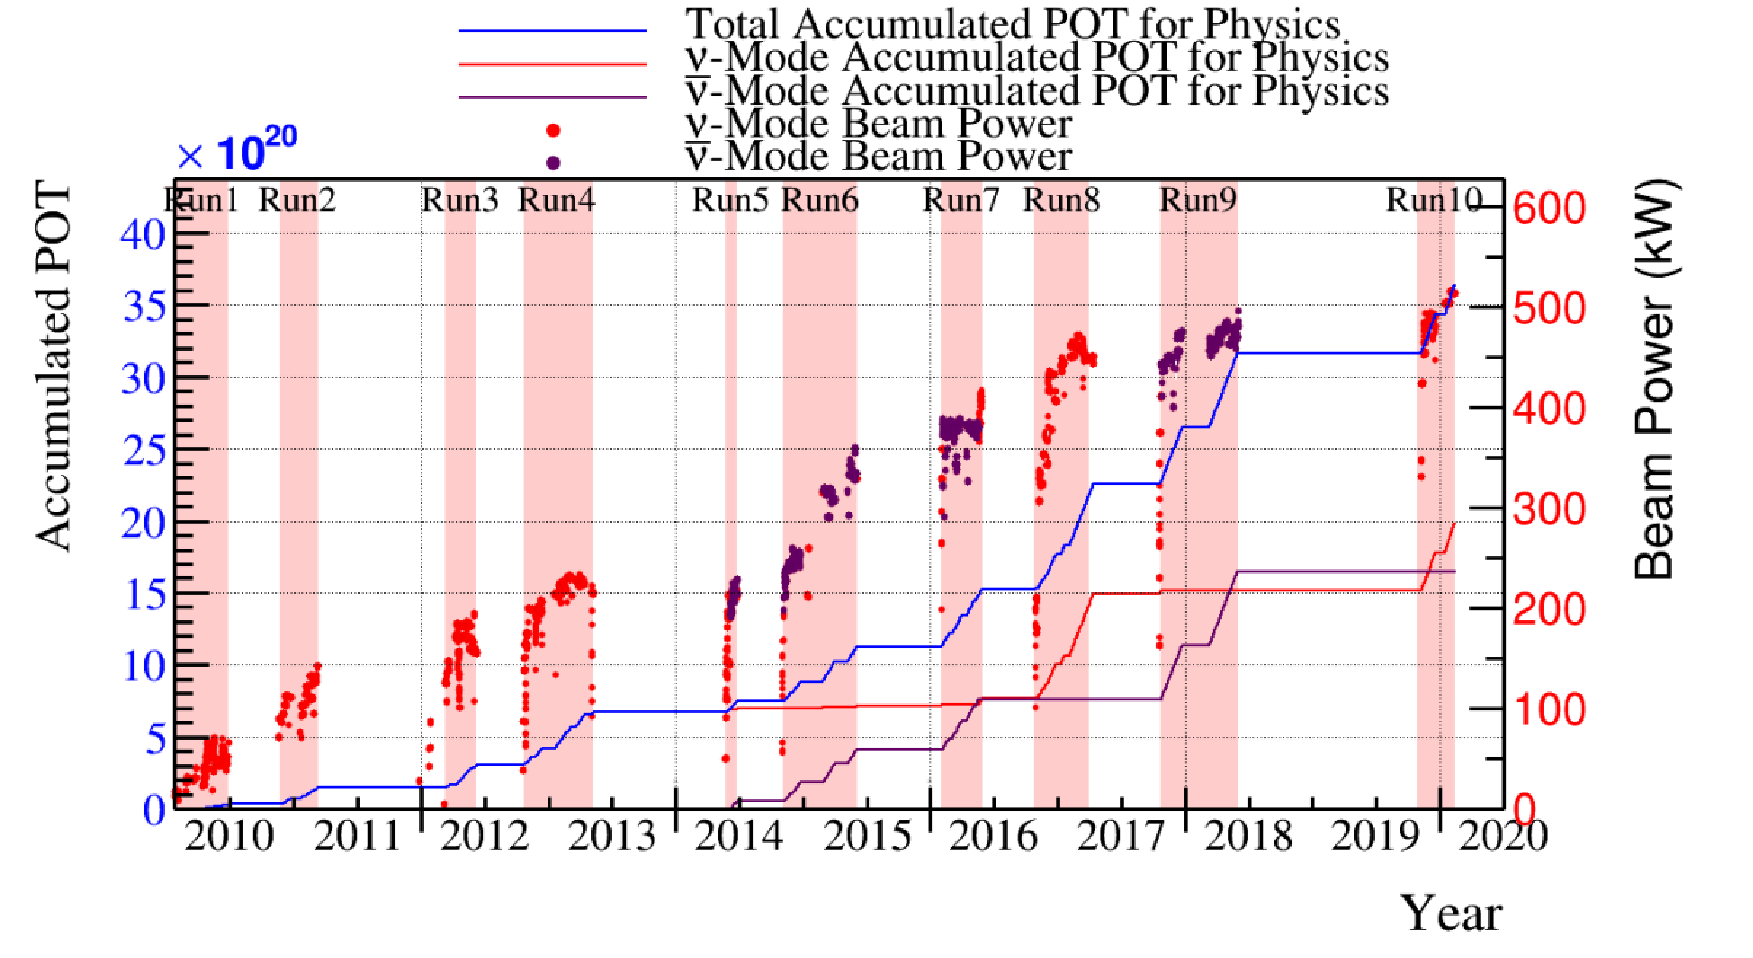
\includegraphics[width=\textwidth, trim={0mm 0mm 0mm 0mm}, clip,page=1]{Figures/Selections/BeamPowerAndPOT.pdf}
  \end{subfigure}
  \caption{The accumulated beam data, measured as the number of protons on target (POT). The total (blue), FHC-only (red), and RHC-only (purple) are given. The beam power is also given by the dot markers. The timescale runs from Run 1 which started in January 2010 until Run 10 which ended in February 2020. The FHC and RHC accumulated data is split \quickmath{54.7\%:45.3\%}.}
  \label{fig:SelsAndSysts_Beam_PowerAndPOT}
\end{figure}

\newpage
\section{Atmospheric Samples}
\label{sec:SelsAndSysts_Sels_Atms}

The atmospheric event selection follows the official SK analysis presented in \cite{Jiang2019-iw} and is documented below. The Monte Carlo prediction used within this analysis corresponds to \quickmath{500} years worth of neutrino events, which is weighted down to match the SK-IV livetime of \quickmath{3244.4} days.

The fully contained (FC), partially contained (PC), and upward going muon events (up-\quickmath{\mu}) which pass the reduction cuts discussed in \autoref{sec:Simulations_Reduction} are further broken down into different samples based on reconstruction information. This section details the samples used within the oscillation analysis, alongside the chosen binning and final spectra used within the fit.

In general, the FC events are first separated by the visible energy deposited within the detector. This is calculated as the sum of the reconstructed kinetic energy above the Cerenkov threshold for all rings present in the event. Events are separated by whether they were above or below \quickmath{E_{vis} = 1.33\text{GeV}}. This separates ``subGeV'' and ``multiGeV'' events. Typically, lower energy events consist of charge current quasi-elastic (CCQE) interactions which are simpler to reconstruct resulting in smaller systematic uncertainties. Events are further separated by the number of rings associated with the event due to similar reasoning. As the oscillation probability is dependent upon the flavour of neutrino, electron and muon events are separated using a similar likelihood method to that discussed in \autoref{sec:Simulation_Reconstruction}. To reduce computational resources required for the reconstruction, only electron and pion hypotheses are considered so this separation cut depends on the ratio of the electron to pion likelihoods. Finally, the number of decay electrons is also used to classify events. As charged current resonant pion production (CCRES) generates a final-state pion that decays to an electron, electron-like events with one decay electron or muon-like events with two decay electrons must have contained a pion in the final state. Consequently, the number of decay electrons is used to target CCQE and CCRES interaction modes. FC subGeV events are then separated into the samples listed in \autoref{tab:SelsAndSysts_Sels_Atms_SubGeV}.

\begin{table}[ht!]
    \centering
    \begin{tabular}{c|l}
      \hline
      Index & Sample \\
      \hline
      0 & \texttt{SubGeV-elike-0dcy} \\
      & \hspace{0.2cm} Single ring \quickmath{e}-like events with zero decay electrons \\ \hline
      1 & \texttt{SubGeV-elike-1dcy} \\
      & \hspace{0.2cm} Single ring \quickmath{e}-like events with one or more decay electrons \\ \hline
      2 & \texttt{SubGeV-mulike-0dcy} \\
      & \hspace{0.2cm} Single ring \quickmath{\mu}-like events with zero decay electrons \\ \hline
      3 & \texttt{SubGeV-mulike-1dcy} \\ 
      & \hspace{0.2cm} Single ring \quickmath{\mu}-like events with one decay electrons \\ \hline
      4 & \texttt{SubGeV-mulike-2dcy} \\
      & \hspace{0.2cm} Single ring \quickmath{\mu}-like events with two or more decay electrons \\ \hline
      5 & \texttt{SubGeV-pi0like} \\
      & \hspace{0.2cm} Two \quickmath{e}-like ring events with zero decay electrons \\
      & \hspace{0.2cm} and reconstructed \quickmath{\pi^{0}} mass \quickmath{85 \leq m_{\pi^{0}} < 215 \text{MeV}} \\
      \hline
      \hline
    \end{tabular}
    \caption{The fully contained subGeV samples used within this oscillation analysis. Both the sample name and description are given.}
    \label{tab:SelsAndSysts_Sels_Atms_SubGeV}
\end{table}

In addition to the cuts discussed above, multiGeV samples also have additional cuts to separate samples which target neutrino and antineutrino separation. As discussed in \autoref{sec:Oscillation_Overview}, the matter resonance only occurs for neutrinos in normal hierarchy and antineutrinos in inverse mass hierarchy so having flavour-enriched samples aids in the determination of the mass hierarchy. For a CCRES interaction,

\begin{align}
  \begin{split}
    \bar{\nu}_e + N \rightarrow e^{+} + N^{'} + &\pi^{-}, \\
    \nu_e + N \rightarrow e^{-} + N^{'} + &\pi^{+} \\
    &\hspace{5pt} \rotatebox[origin=c]{180}{$\Lsh$} \hspace{5pt} \mu^{+} + \nu_\mu \\
    &\hspace{20pt} \rotatebox[origin=c]{180}{$\Lsh$} \hspace{5pt} e^{+} + \nu_e + \bar{\nu}_\mu.
\end{split}
\end{align}

Where the \quickmath{\pi^{-}} emitted from a \quickmath{\bar{\nu_{e}}} interaction is more likely to be absorbed within the oxygen nucleus \cite{LeeKaPik} compared to the \quickmath{\pi^{+}} from \quickmath{\nu_{e}} interactions. Consequently, the number of tagged decay electrons associated with an event gives an indication of whether the interaction was due to a neutrino or antineutrino: zero for \quickmath{\bar{\nu}_{e}} events, and one or more for \quickmath{\nu_{e}} events. The ability to separate neutrino from antineutrino events is illustrated in \autoref{tab:SelsAndSysts_Sels_AtmPurity}, where the \texttt{MultiGeV-elike-nue} has \quickmath{78\%} purity enhancement of neutrino events with only \quickmath{7\%} antineutrino background in that sample.

This relatively simple discriminator works reasonably well for single-ring events. However, this is not the case for multi-ring events. A multi-GeV multi-ring separation (MME) likelihood cut which specifically targets multiGeV multiRing electron-like events was introduced in \cite{PhysRevD.81.092004, PhysRevD.74.032002}. Four observables are used within this likelihood cut: the number of decay electrons, the maximum distance between the vertex of the neutrino and the decay electrons, the energy deposited by the leading energy ring, and the reconstructed particle identification of that highest energy ring. The last three variables are selected based on typical event kinematics comparing CC\quickmath{\nu_{e}} events to the CC\quickmath{\nu_{\mu}} and NC backgrounds. Typically, more energy is carried by the hadronic system in these background interactions and the distance cut targets the decay of muons from CC\quickmath{\nu_{\mu}}, which tend to travel further than the pions from CC\quickmath{\nu_{e}} interactions.

\begin{table}[ht!]
    \centering
    \begin{tabular}{c|l}
      \hline
      Index & Sample \\
      \hline
      0 & \texttt{MultiGeV-elike-nue} \\
      & \hspace{0.2cm} Single ring \quickmath{e}-like events with zero decay electrons \\ \hline
      1 & \texttt{MultiGeV-elike-nuebar} \\
      & \hspace{0.2cm} Single ring \quickmath{e}-like events with one or more decay electrons \\ \hline
      2 & \texttt{MultiGeV-mulike} \\
      & \hspace{0.2cm} Single ring \quickmath{\mu}-like events \\ \hline
      3 & \texttt{MultiRing-elike-nue} \\
      & \hspace{0.2cm} Two or more ring events with leading energy \quickmath{e}-like ring \\ 
      & \hspace{0.2cm} and passed both MME and \quickmath{\nu/\bar{\nu}} separation likelihood cuts\\ \hline
      4 & \texttt{MultiRing-elike-nuebar} \\
      & \hspace{0.2cm} Two or more ring events with leading energy \quickmath{e}-like ring \\ 
      & \hspace{0.2cm} and passed MME and failed \quickmath{\nu/\bar{\nu}} separation likelihood cuts\\ \hline
      5 & \texttt{MultiRing-mulike} \\
      & \hspace{0.2cm} Two or more ring events with leading energy \quickmath{\mu}-like ring \\ 
      & \hspace{0.2cm} and only requires \quickmath{E_{vis} > 0.6\text{GeV}} \\ \hline
      6 & \texttt{MultiRing-Other1} \\
      & \hspace{0.2cm} Two or more ring events with leading energy \quickmath{e}-like ring \\ 
      & \hspace{0.2cm} and failed the MME likelihood cut \\ 
      \hline
      \hline
    \end{tabular}
    \caption{The fully contained multiGeV samples used within this oscillation analysis. Both the sample name and description are given.}
    \label{tab:SelsAndSysts_Sels_Atms_MultiGeV}
\end{table}

Neutrino and antineutrino events are then separated by a second likelihood method (\quickmath{\nu/\bar{\nu}} separation) detailed in \cite{Kamiokande_Collaboration2017-nf}. This uses the number of decay electrons, the number of reconstructed rings, and the event's transverse momentum. As discussed above, positively changed pions from neutrino interactions are less likely to be absorbed. For this high-energy sample, the majority of those pions will be above the Cherenkov threshold which results in more rings compared to an antineutrino interaction. The angular distribution also tends to be more forward peaked in antineutrino interactions. The FC multiGeV sample definitions are detailed in \autoref{tab:SelsAndSysts_Sels_Atms_MultiGeV}.

The PC and up-\quickmath{\mu} events are split by the amount of energy deposited within the outer detector, into ``stopping'' and ``through-going'' samples. If an event leaves the detector, the energy it takes with it has to be estimated which increases the systematic uncertainty compared to events entirely contained within the inner detector. The through-going up-\quickmath{\mu} are further separated by the presence of any electromagnetic showering in the event, as the assumption of non-showering muon does not give reliable reconstruction for these types of events \cite{Ashie_2005}. In total, \quickmath{13} FC, \quickmath{2} PC, and \quickmath{3} up-\quickmath{\mu} atmospheric samples are included within this analysis.

\begin{table}[ht!]
    \centering
    \begin{tabular}{l|c|c|c|c|c}
      \hline
      Sample & CC\quickmath{\nu_{e}} & CC\quickmath{\bar{\nu}_{e}} & CC(\quickmath{\nu_{\mu} + \bar{\nu}_{\mu}}) & CC(\quickmath{\nu_{\tau}+\bar{\nu}_{\tau}}) & NC \\
      \hline
      \texttt{SubGeV-elike-0dcy} & \quickmath{72.17} & \quickmath{23.3} & \quickmath{0.724} & \quickmath{0.033} & \quickmath{3.77} \\
      \texttt{SubGeV-elike-1dcy} & \quickmath{86.81} & \quickmath{1.773} & \quickmath{7.002} & \quickmath{0.062} & \quickmath{4.351} \\
      \texttt{SubGeV-mulike-0dcy} & \quickmath{1.003} & \quickmath{0.380} & \quickmath{90.07} & \quickmath{0.036} & \quickmath{8.511} \\
      \texttt{SubGeV-mulike-1dcy} & \quickmath{0.023} & \quickmath{0.} & \quickmath{98.46} & \quickmath{0.029} & \quickmath{1.484} \\
      \texttt{SubGeV-mulike-2dcy} & \quickmath{0.012} & \quickmath{0.} & \quickmath{99.25} & \quickmath{0.030} & \quickmath{0.711} \\
      \texttt{SubGeV-pi0like} & \quickmath{6.923} & \quickmath{2.368} & \quickmath{0.928} & \quickmath{0.011} & \quickmath{89.77} \\
      \texttt{MultiGeV-elike-nue} & \quickmath{78.18} & \quickmath{7.041} & \quickmath{3.439} & \quickmath{1.886} & \quickmath{9.451} \\
      \texttt{MultiGeV-elike-nuebar} & \quickmath{56.68} & \quickmath{37.81} & \quickmath{0.174} & \quickmath{0.614} & \quickmath{4.718} \\
      \texttt{MultiGeV-mulike} & \quickmath{0.024} & \quickmath{0.005} & \quickmath{99.67} & \quickmath{0.245} & \quickmath{0.058} \\
      \texttt{MultiRing-elike-nue} & \quickmath{59.32} & \quickmath{12.39} & \quickmath{4.906} & \quickmath{3.385} & \quickmath{20} \\
      \texttt{MultiRing-elike-nuebar} & \quickmath{52.39} & \quickmath{31.03} & \quickmath{1.854} & \quickmath{1.585} & \quickmath{13.14} \\
      \texttt{MultiRing-mulike} & \quickmath{0.673} & \quickmath{0.080} & \quickmath{97.33} & \quickmath{0.342} & \quickmath{1.578} \\
      \texttt{MultiRingOther-1} & \quickmath{27.98} & \quickmath{2.366} & \quickmath{34.93} & \quickmath{4.946} & \quickmath{29.78} \\
      \texttt{PCStop} & \quickmath{8.216} & \quickmath{3.118} & \quickmath{84.45} & \quickmath{0.} & \quickmath{4.214} \\
      \texttt{PCThru} & \quickmath{0.564} & \quickmath{0.207} & \quickmath{98.65} & \quickmath{0.} & \quickmath{0.576} \\
      \texttt{UpStop-mu} & \quickmath{0.829} & \quickmath{0.370} & \quickmath{98.51} & \quickmath{0.} & \quickmath{0.289} \\
      \texttt{UpThruNonShower-mu} & \quickmath{0.206} & \quickmath{0.073} & \quickmath{99.62} & \quickmath{0.} & \quickmath{0.103} \\
      \texttt{UpThruShower-mu} & \quickmath{0.128} & \quickmath{0.054} & \quickmath{99.69} & \quickmath{0.} & \quickmath{0.132} \\
      \hline
      \hline
    \end{tabular}
    \caption{The purity of each atmospheric sample used within this analysis, broken down by charged current (CC) and neutral current (NC) interactions and which neutrino flavour interacted within the detector. The pre-fit dial values and Asimov A oscillation parameter sets are assumed. Electron neutrino and antineutrino events are separated to illustrate the ability of the separation likelihood cuts used within the sample selections.}
    \label{tab:SelsAndSysts_Sels_AtmPurity}
\end{table}

\begin{table}[ht!]
    \centering
    \begin{tabular}{l|c|c}
      \hline
      Sample & \quickmath{\cos(\theta_{Z})} Bins & Momentum Bin Edges (\quickmath{\log_{10}(P) \text{ MeV}}) \\
      \hline
      \texttt{SubGeV-elike-0dcy} & 10 & 2.0, 2.4, 2.6, 2.8, 3.0, 3.2 \\
      \texttt{SubGeV-elike-1dcy} & 1 & 2.0, 2.4, 2.6, 2.8, 3.0, 3.2 \\
      \texttt{SubGeV-mulike-0dcy} & 10 & 2.0, 2.4, 2.6, 2.8, 3.0, 3.2 \\
      \texttt{SubGeV-mulike-1dcy} & 10 & 2.0, 2.4, 2.6, 2.8, 3.0, 3.2 \\
      \texttt{SubGeV-mulike-2dcy} & 1 & 2.0, 2.4, 2.6, 2.8, 3.0, 3.2 \\
      \texttt{SubGeV-pi0like} & 1 & 2.0, 2.2, 2.4, 2.6, 2.8, 3.2 \\
      \texttt{MultiGeV-elike-nue} & 10 & 3.0, 3.4, 3.7, 4.0, 5.0 \\
      \texttt{MultiGeV-elike-nuebar} & 10 & 3.0, 3.4, 3.7, 4.0, 5.0 \\
      \texttt{MultiGeV-mulike} & 10 & 3.0, 3.4, 5.0 \\
      \texttt{MultiRing-elike-nue} & 10 & 3.0, 3.4, 3.7, 5.0 \\
      \texttt{MultiRing-elike-nuebar} & 10 & 3.0, 3.4, 3.7, 5.0 \\
      \texttt{MultiRing-mulike} & 10 & 2.0, 3.124, 3.4, 3.7, 5.0 \\
      \texttt{MultiRing-Other1} & 10 & 3.0, 3.4, 3.7, 4.0, 5.0 \\
      \texttt{PC-Stop} & 10 & 2.0, 3.4, 5.0\\
      \texttt{PC-Through} & 10 & 2.0, 3.124, 3.4, 3.7, 5.0 \\
      \texttt{Upmu-Stop} & 10 & 3.2, 3.4, 3.7, 8.0 \\
      \texttt{Upmu-Through-Showering} & 10 & 2.0, 8.0 \\
      \texttt{Upmu-Through-NonShowering} & 10 & 2.0, 8.0 \\
      \hline
      \hline
    \end{tabular}
    \caption{The reconstructed cosine zenith and lepton momentum binning assigned to the atmospheric samples. The ``\quickmath{\cos(\theta_{Z})} Bins'' column illustrates the number of bins uniformly distributed over the \quickmath{-1.0 \leq \cos(\theta_{Z}) \leq 1.0} region for fully and partially contained samples and \quickmath{-1.0 \leq \cos(\theta_{Z}) \leq 0.0} region for up-\quickmath{\mu} samples.}
    \label{tab:SelsAndSysts_Sels_Atms_Binning}
\end{table}

The atmospheric samples are binned in reconstructed lepton momentum and direction, as given by \autoref{tab:SelsAndSysts_Sels_Atms_Binning}. The distribution of the reconstructed lepton momentum (for samples that only have one bin reconstructed zenith angle) and reconstructed direction for each atmospheric sample used within this analysis is illustrated in \autoref{fig:SelsAndSysts_AllSampleComparison}.

\begin{sidewaysfigure}
  \centering
  \begin{subfigure}[t]{\textwidth}
    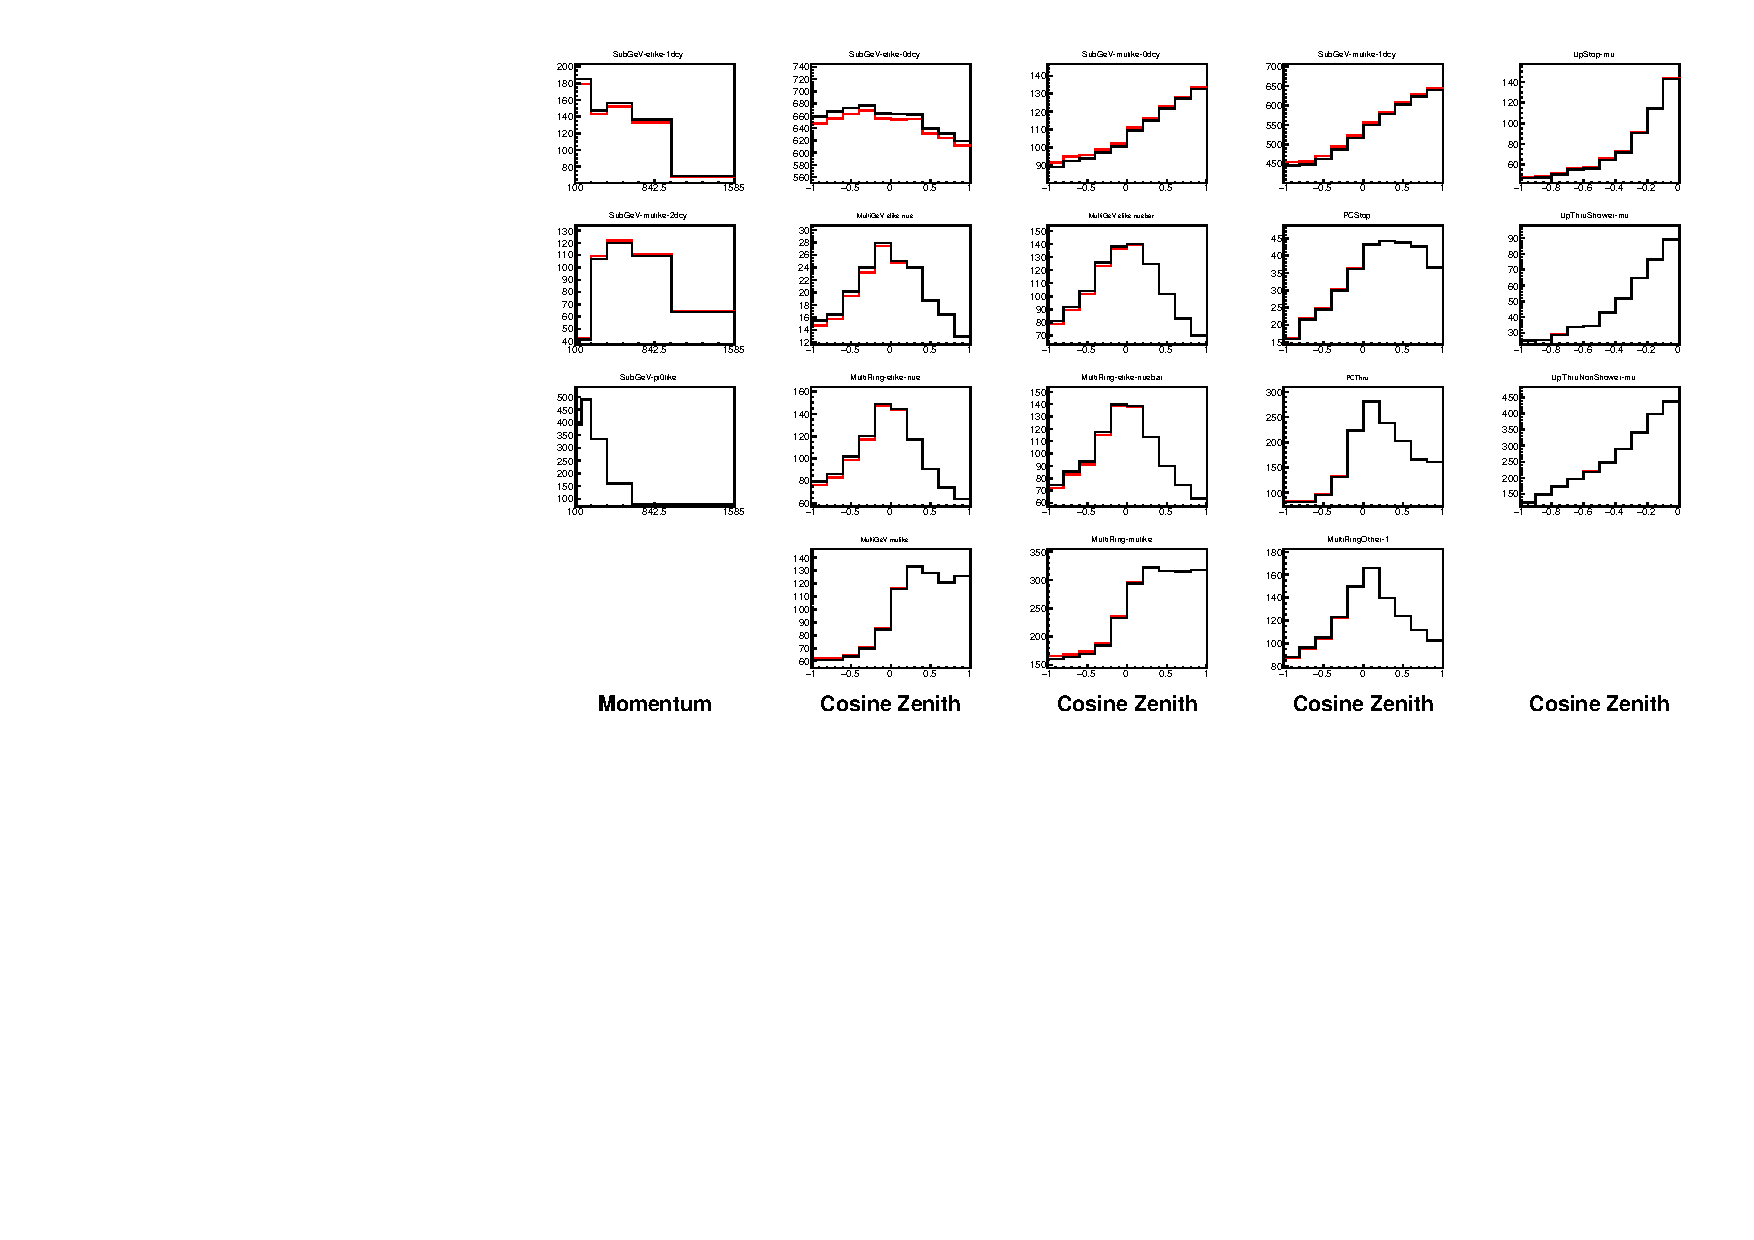
\includegraphics[width=\textwidth, trim={0mm 0mm 0mm 0mm}, clip,page=1]{Figures/Selections/HistogramComparison.pdf}
  \end{subfigure}
  \caption{Comparison of the SK-IV atmospheric samples between predictions made with the Asimov A (Black) and Asimov B (Red) oscillation parameter sets, given in \autoref{tab:Theory_ParameterSets}. The subGeV samples CCRES and \quickmath{\pi^{0}}-like samples are given in their reconstructed lepton momentum. All other samples are presented in their reconstructed zenith angle projection.}
  \label{fig:SelsAndSysts_AllSampleComparison}
\end{sidewaysfigure}

\clearpage
\section{Near Detector Beam Samples}
\label{sec:SelsAndSysts_Sels_ND}

The near detector sample selections are documented in detail within \cite{t2k_tn_395} and summarised below. Samples are selected based upon the particular Fine Grained Detector (FGD) (see \autoref{subsec:T2KSKExp_T2K_ND280}) the neutrino interacted within as well as the operating mode of the beam. For more substantial constraints on cross-section model parameters, wrong-sign neutrino samples are also considered when the beam is operating in RHC (antineutrino) mode. Samples from the wrong-sign component of the FHC beam mode are not included as they are statistically insignificant compared to those already listed.

Before being assigned a sample, all events must undergo CC-inclusive cuts, as defined in TN212.

\begin{itemize}
\item Event Timing: The DAQ must be operational and the event must occur within the expected time window
\item TPC Requirement: The track path must intercept one or more TPCs
\item Fiducial volume: The event must originate from within a fiducial volume
\item Upstream Background: Remove reconstruction failures occurring from muons that originate upstream of the FGDs by requiring no high-momentum tracks within \quickmath{150\text{mm}} of the candidate vertex. Additionally, events that occur within the downstream FGD are vetoed if a secondary track starts within the upstream FGD
\item Broken track removal: All candidates where the muon candidate is broken in two tracks are removed
\item Muon PID: Measurements of \quickmath{dE/dx} in a TPC are used to distinguish muon-like events using a likelihood cut
\end{itemize}

In addition to these cuts, the RHC neutrino events also have to undergo the following cuts to aid in the separation of neutrino and antineutrino TN246:

\begin{itemize}
\item TPC Requirement: The track path must intercept TPC2
\item Positive Track: The highest momentum track must be positive
\item TPC1 Veto: Remove any events originating upstream of TPC1
\end{itemize}

Once all CC-inclusive events have been determined, they are further segregated into sub-samples that target the constraints on interaction modes most relevant at the far detector. These are CC\quickmath{0\pi}, CC\quickmath{1\pi}, and CCOther, which target CCQE, CCRES, and other CC background interactions. They are defined with the following cuts:

\begin{itemize}
\item \textbf{\quickmath{\nu_{\mu} \text{CC} 0\pi} Selection}: No electrons in TPC and no charged pions or decay electrons within the TPC or FGD
\item \textbf{\quickmath{\nu_{\mu} \text{CC} 1\pi} Selection}: Exactly one charged pion pion in either the TPC or FGD, where the number of charged pions in the FGD is equal to the number of decay electrons
\item \textbf{\quickmath{\nu_{\mu} \text{CCOther}} Selection}: All events which are not classified into the above two selections. These contain neutral pion and multiple charged pion events.
\end{itemize}

Counting the three selections for each FGD in neutrino (FHC) and anti-neutrino (RHC) running, including the wrong-sign background in RHC, 18 near detector samples are used within this analysis. These samples are binned in reconstructed lepton momentum (illustrated in \autoref{fig:SelsAndSysts_Beam_NDPred}) and direction with respect to the beam. The binning is chosen such that each event has at least \quickmath{20} Monte Carlo events in each bin. This is to ensure that the bins are coarse enough to ensure the reduction of statistical errors, whilst also being fine enough to sample the high-resolution peak regions. The binning and choice of non-uniform binning are detailed in \cite{thesis_will}.

\begin{figure}[h]
  \begin{subfigure}[t]{0.49\textwidth}
    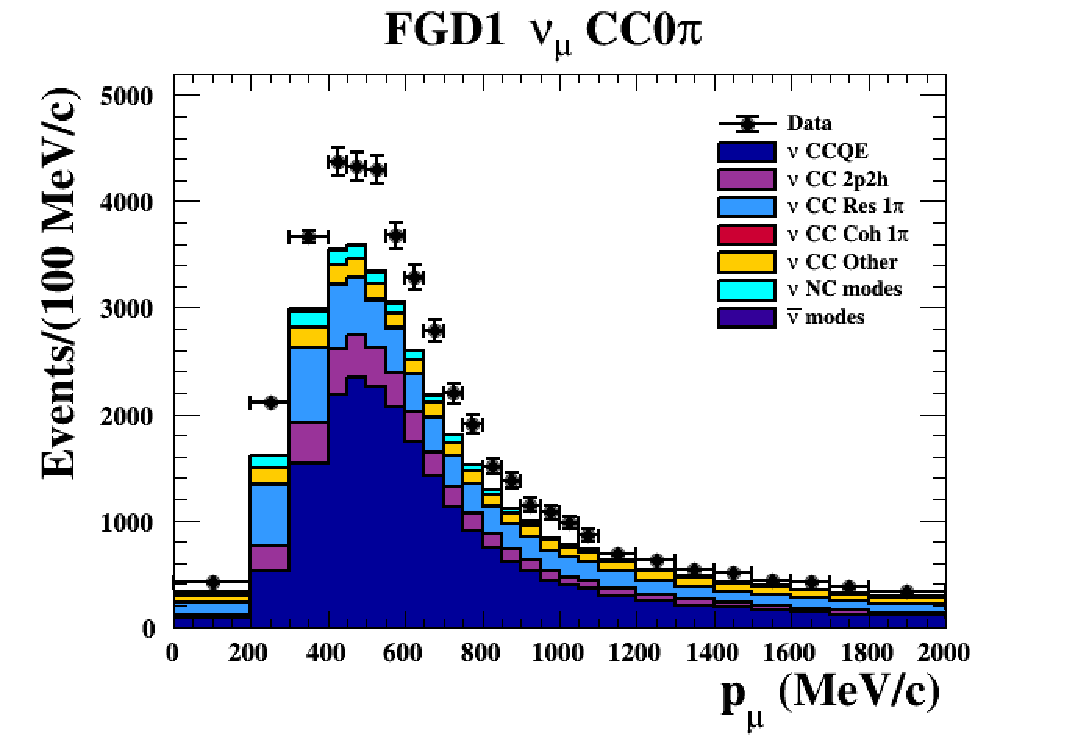
\includegraphics[width=\textwidth, trim={0mm 0mm 0mm 0mm}, clip,page=1]{Figures/Selections/Pmu_1D_modes_FGD1_numuCC_0pi_Data_prefit.pdf}
    %\subcaption{FGD1 FHC \quickmath{\nu_{\mu} 0\pi}}
  \end{subfigure}%
  \begin{subfigure}[t]{0.49\textwidth}
    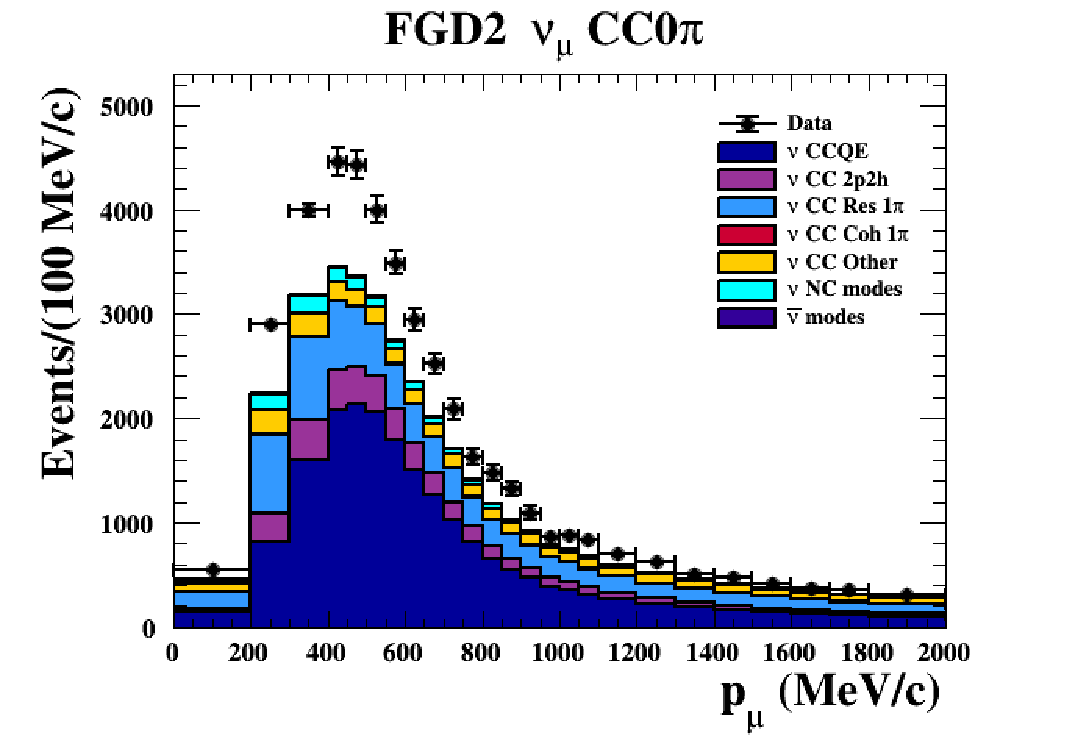
\includegraphics[width=\textwidth, trim={0mm 0mm 0mm 0mm}, clip,page=1]{Figures/Selections/Pmu_1D_modes_FGD2_numuCC_0pi_Data_prefit.pdf}
    %\subcaption{FGD2 FHC \quickmath{\nu_{\mu} 0\pi}}
  \end{subfigure}
  \begin{subfigure}[t]{0.49\textwidth}
    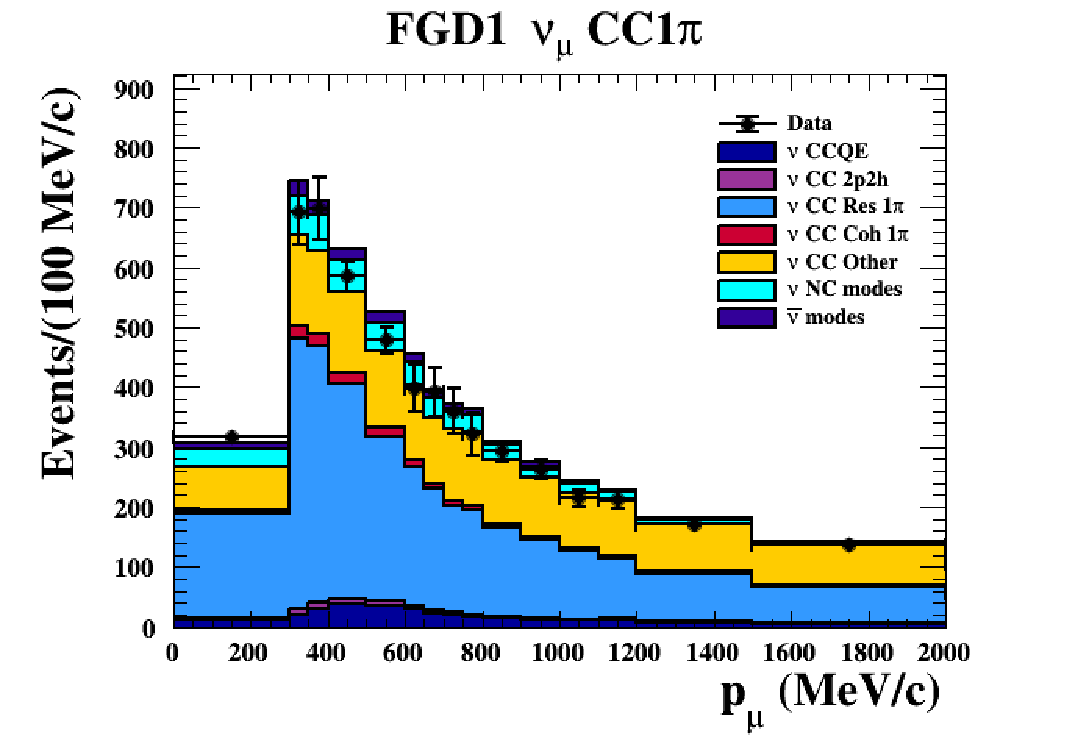
\includegraphics[width=\textwidth, trim={0mm 0mm 0mm 0mm}, clip,page=1]{Figures/Selections/Pmu_1D_modes_FGD1_numuCC_1pi_Data_prefit.pdf}
    %\subcaption{FGD1 FHC \quickmath{\nu_{\mu} 1\pi}}
  \end{subfigure}%
  \begin{subfigure}[t]{0.49\textwidth}
    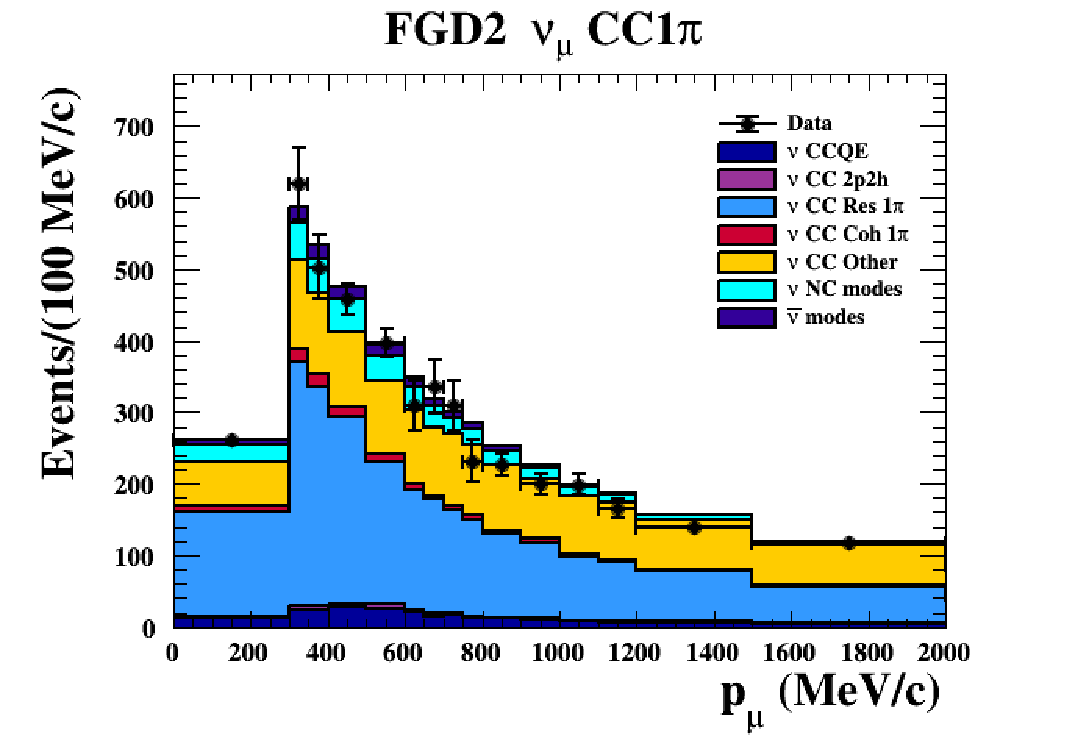
\includegraphics[width=\textwidth, trim={0mm 0mm 0mm 0mm}, clip,page=1]{Figures/Selections/Pmu_1D_modes_FGD2_numuCC_1pi_Data_prefit.pdf}
    %\subcaption{FGD2 FHC \quickmath{\nu_{\mu} 1\pi}}
  \end{subfigure}
  \begin{subfigure}[t]{0.49\textwidth}
    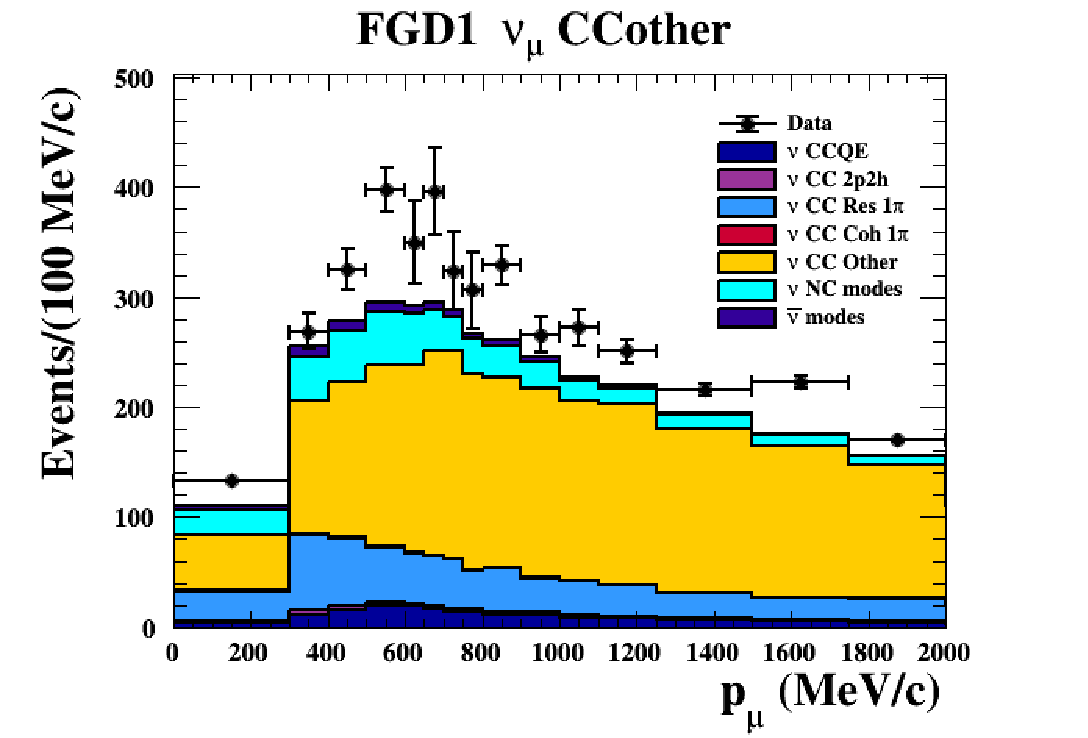
\includegraphics[width=\textwidth, trim={0mm 0mm 0mm 0mm}, clip,page=1]{Figures/Selections/Pmu_1D_modes_FGD1_numuCC_other_Data_prefit.pdf}
    %\subcaption{FGD1 FHC \quickmath{\nu_{\mu} \text{Other}}}
  \end{subfigure}%
  \begin{subfigure}[t]{0.49\textwidth}
    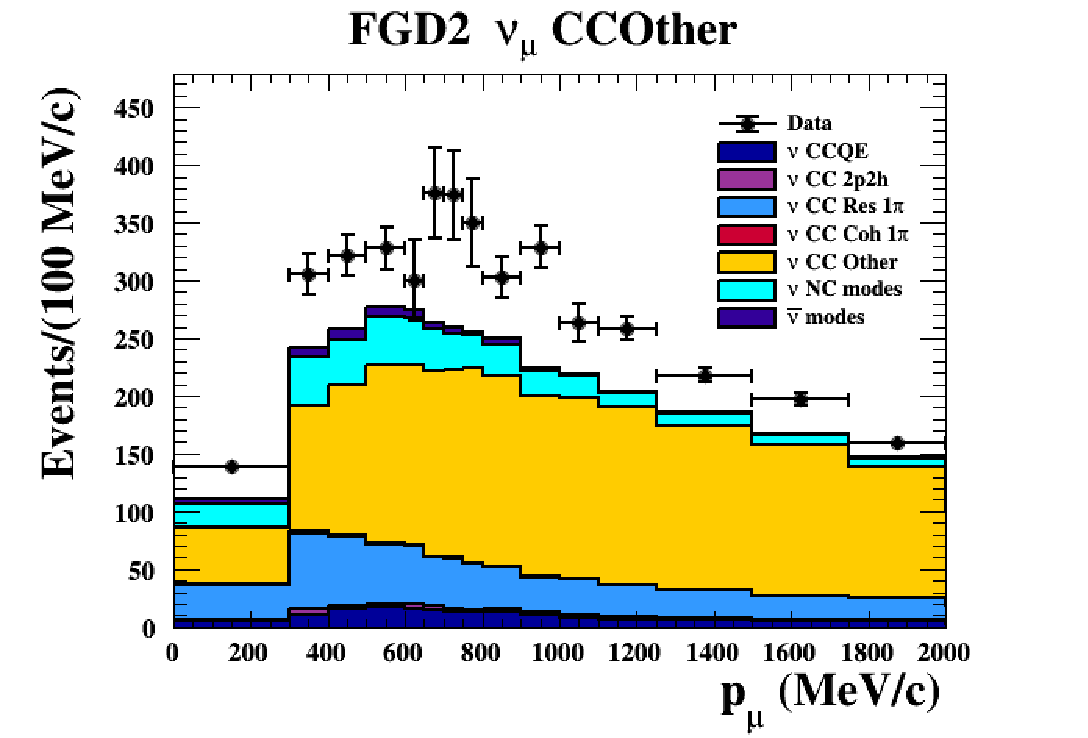
\includegraphics[width=\textwidth, trim={0mm 0mm 0mm 0mm}, clip,page=1]{Figures/Selections/Pmu_1D_modes_FGD2_numuCC_other_Data_prefit.pdf}
    %%\subcaption{FGD2 FHC \quickmath{\nu_{\mu} \text{Other}}}
  \end{subfigure}
  \caption{The nominal Monte Carlo predictions for the FGD1 and FGD2 samples in neutrino beam mode (FHC), broken down into the \quickmath{CC\nu_{\mu} 0\pi}, \quickmath{CC\nu_{\mu} 1\pi} and \quickmath{CC\nu_{\mu} \text{ Other}} categories. Figures taken from \cite{t2k_tn_395}.}
  \label{fig:SelsAndSysts_Beam_NDPred}
\end{figure}

\section{Far Detector Beam Samples}
\label{sec:SelsAndSysts_Sels_FD}

The beam neutrino events which occur at the SK detector, which pass the reduction cuts detailed in \autoref{sec:Simulations_Reduction}, are separated depending on whether the beam was operating in neutrino or antineutrino mode. The events are then segregated into three separate samples: electron-like (\quickmath{1\text{R}e}), muon-like (\quickmath{1\text{R}\mu}), and CC\quickmath{1\pi^{+}}-like which are observed as electron-like events with an associated decay electron. As discussed in \autoref{sec:SelsAndSysts_Sels_Atms}, positively charged pions from emitted from neutrino interactions are less likely to be absorbed by oxygen nuclei and thus are more likely to produce events that are observed with an associated decay electron. Consequently, the CC\quickmath{1\pi^{+}}-like sample is only selected when the beam is operating in FHC-neutrino mode. Therefore, five beam samples measured at SK are used in this analysis. As the T2K oscillation analysis has evolved over the years and the selections changed, the sample names are suffixed with \texttt{2020} to indicate they are the samples used within the 2020 T2K oscillation analysis.

The fiducial volume definition for beam samples is slightly different from that used within the atmospheric samples.  It uses both the distance to the closest wall (\texttt{dWall}) and the distance to the wall along the trajectory of the particle (\texttt{toWall}). This allows events that originate close to the wall but are facing into the tank to be included within the analysis, which would have otherwise been removed. The exact cut values for both \texttt{dWall} and \texttt{toWall} are different for each of the three types of sample and optimised based on T2K sensitivity to \dcp \cite{t2k_tn_318, t2k_tn_319}.

\paragraph{\quickmath{1\text{R}e} event selection}

For an event to be classified as a \quickmath{1\text{R}e}-like, the event must follow:

\begin{itemize}
\item Fully-contained and within \texttt{dWall} \quickmath{>80\text{cm}} and \texttt{toWall} \quickmath{>170\text{cm}}
\item Total of one ring which is reconstructed as electron-like with reconstructed momentum \quickmath{P_{e} > 100\text{MeV}}
\item Zero decay electrons are associated with the event
\item Passes \quickmath{\pi^{0}} rejection cut discussed in \autoref{sec:Simulation_Reconstruction}
\end{itemize}

The zero decay electron cut specifically targets CCQE interactions and the \quickmath{\pi^{0}} rejection cut it designed to remove neutral current \quickmath{\pi^{0}} background events as they can be easily reconstructed as \quickmath{1\quickmath{R}e} events without this cut.

\paragraph{CC\quickmath{1\pi^{+}} event selection} This event selection is very similar to that of the \quickmath{1\text{R}e} sample. The only difference is that the \texttt{dWall} and \texttt{toWall} criteria are shifted to \quickmath{>50\text{cm}} and \quickmath{>270\text{cm}}, respectively. Furthermore, exactly one decay electron is required from the \quickmath{\pi^{+}} decay. 

\paragraph{\quickmath{1\text{R}\mu} event selection}

A \quickmath{1\text{R}e}-like event is determined by the following cuts:

\begin{itemize}
\item Fully-contained and within \texttt{dWall} \quickmath{>50\text{cm}} and \texttt{toWall} \quickmath{>250\text{cm}}
\item Total of one ring which is reconstructed as muon-like with reconstructed momentum \quickmath{P_{\mu} > 200\text{MeV}}
\item Fewer than two decay electrons are associated with the event
\item Passes \quickmath{\pi^{+}} rejection cut discussed in \autoref{sec:Simulation_Reconstruction}
\end{itemize}

As pions and muons have similar masses, the Cherenkov rings they generate have similar opening angles. Consequently, to select muons, the events have to pass the \quickmath{\pi^{+}} rejection cut which is specifically optimised to separate the two types of events.

All of these samples are binned in reconstructed neutrino energy. This is possible as the direction from the source is known extremely well, unlike atmospheric neutrinos. This value is calculated for the \quickmath{1\text{R}e} and \quickmath{1\text{R}\mu} samples assuming CCQE interactions,

\begin{equation}
  \label{sec:SelsAndSysts_Erec_CCQE}
  E^{rec}_{\nu} = \frac{(M_{N}-V_{nuc})E_{l} - m_{l}^{2}/2 + M_{N}V_{nuc} - V_{nuc}^{2}/2 + (M_{P}^{2} + M_{N}^{2})/2}{M_{N} - V_{nuc} - E_{l} + P_{l}\cos(\theta_{beam})}
\end{equation}

Where \quickmath{M_{N}}, \quickmath{M_{P}} and \quickmath{m_{l}} are the masses of the neutron, proton and outgoing lepton, respectively. \quickmath{V_{nuc} = 27\text{MeV}} is the binding energy of the oxygen nuclei, \quickmath{\theta_{beam}} is the angle between the beam and the direction of the outgoing lepton, and \quickmath{E_{l}} and \quickmath{P_{l}} are the energy and momentum of that outgoing lepton.

\begin{figure}[h]
  \begin{subfigure}[t]{0.49\textwidth}
    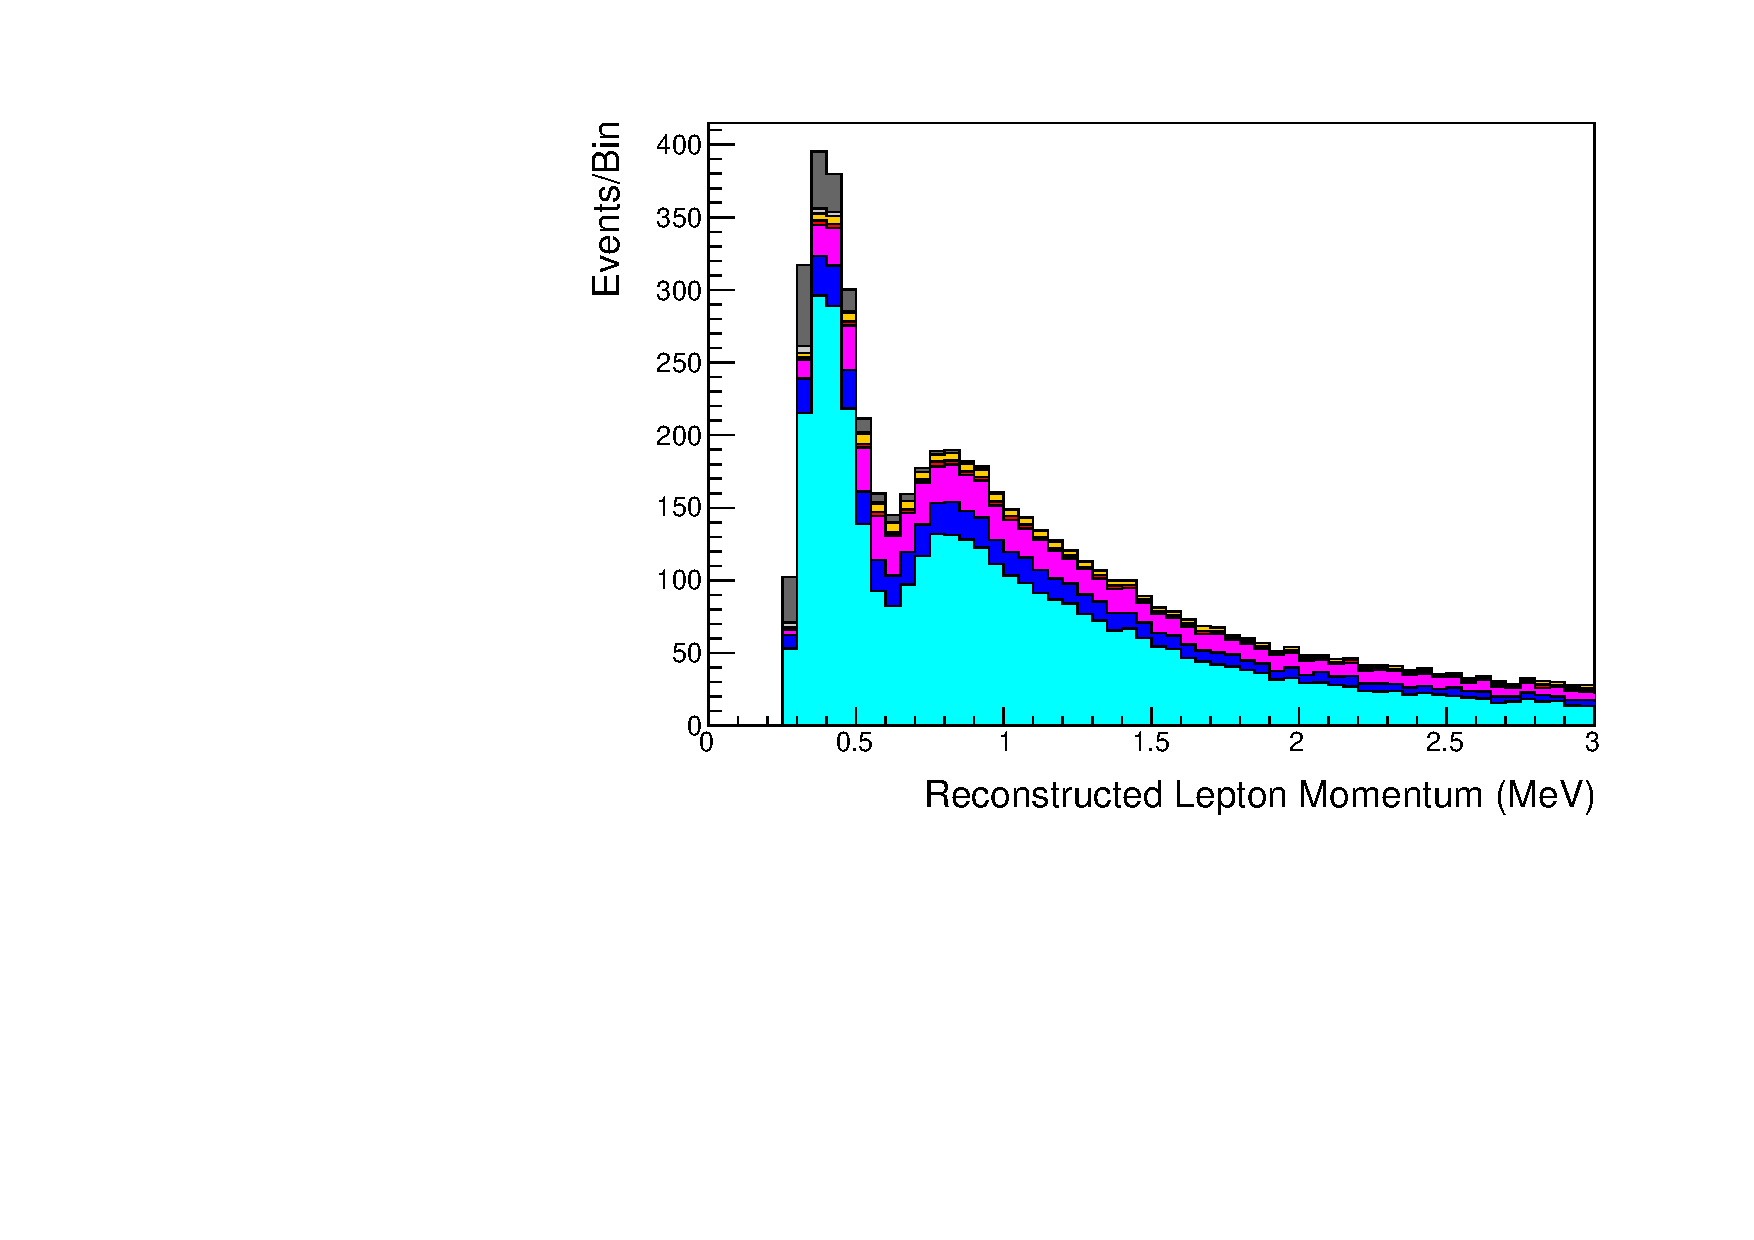
\includegraphics[width=\textwidth, trim={0mm 0mm 0mm 0mm}, clip,page=1]{Figures/Selections/FHC1Rmu-2020_X.pdf}
    \subcaption{FHC \quickmath{1\text{R}\mu}}
  \end{subfigure}%
  \begin{subfigure}[t]{0.49\textwidth}
    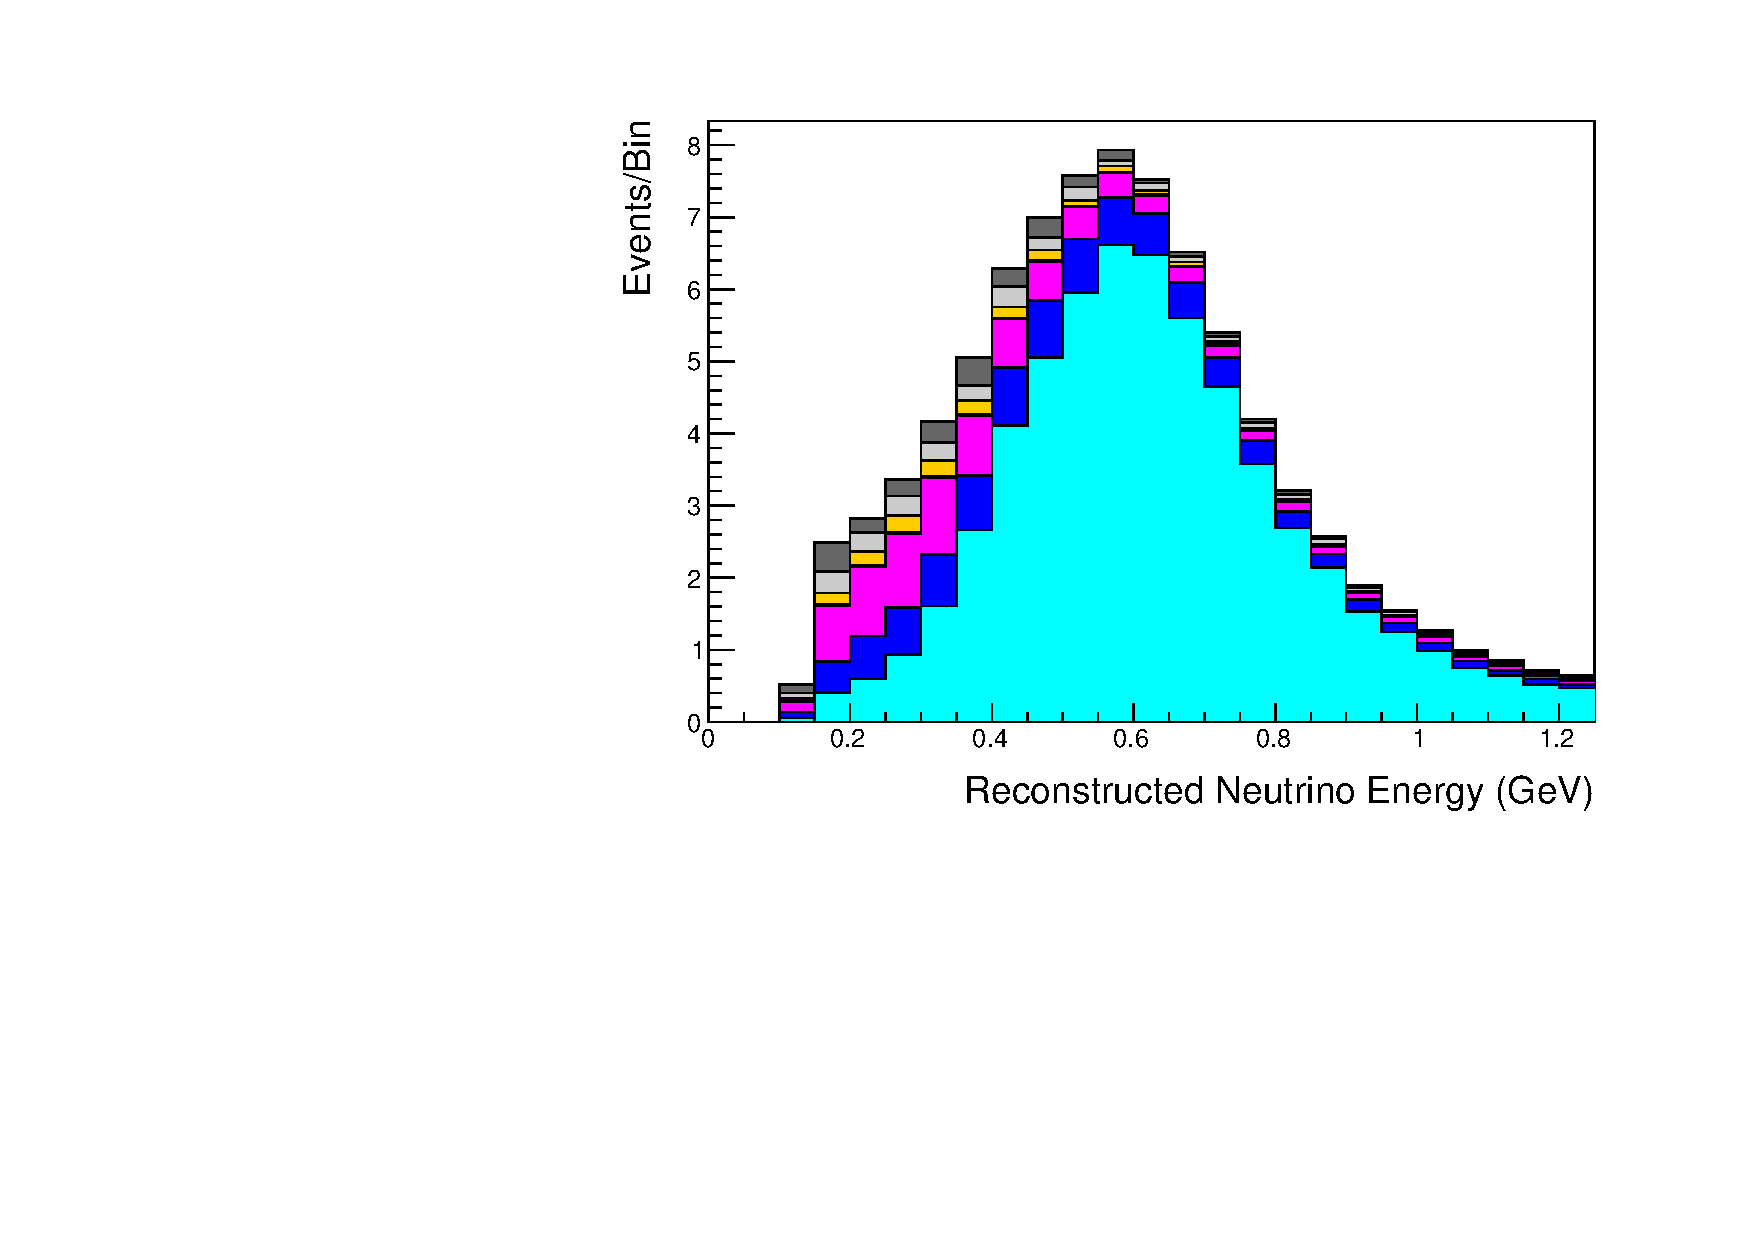
\includegraphics[width=\textwidth, trim={0mm 0mm 0mm 0mm}, clip,page=1]{Figures/Selections/FHC1Re-2020_X.pdf}
    \subcaption{FHC \quickmath{1\text{R}e}}
  \end{subfigure}
  \begin{subfigure}[t]{0.49\textwidth}
    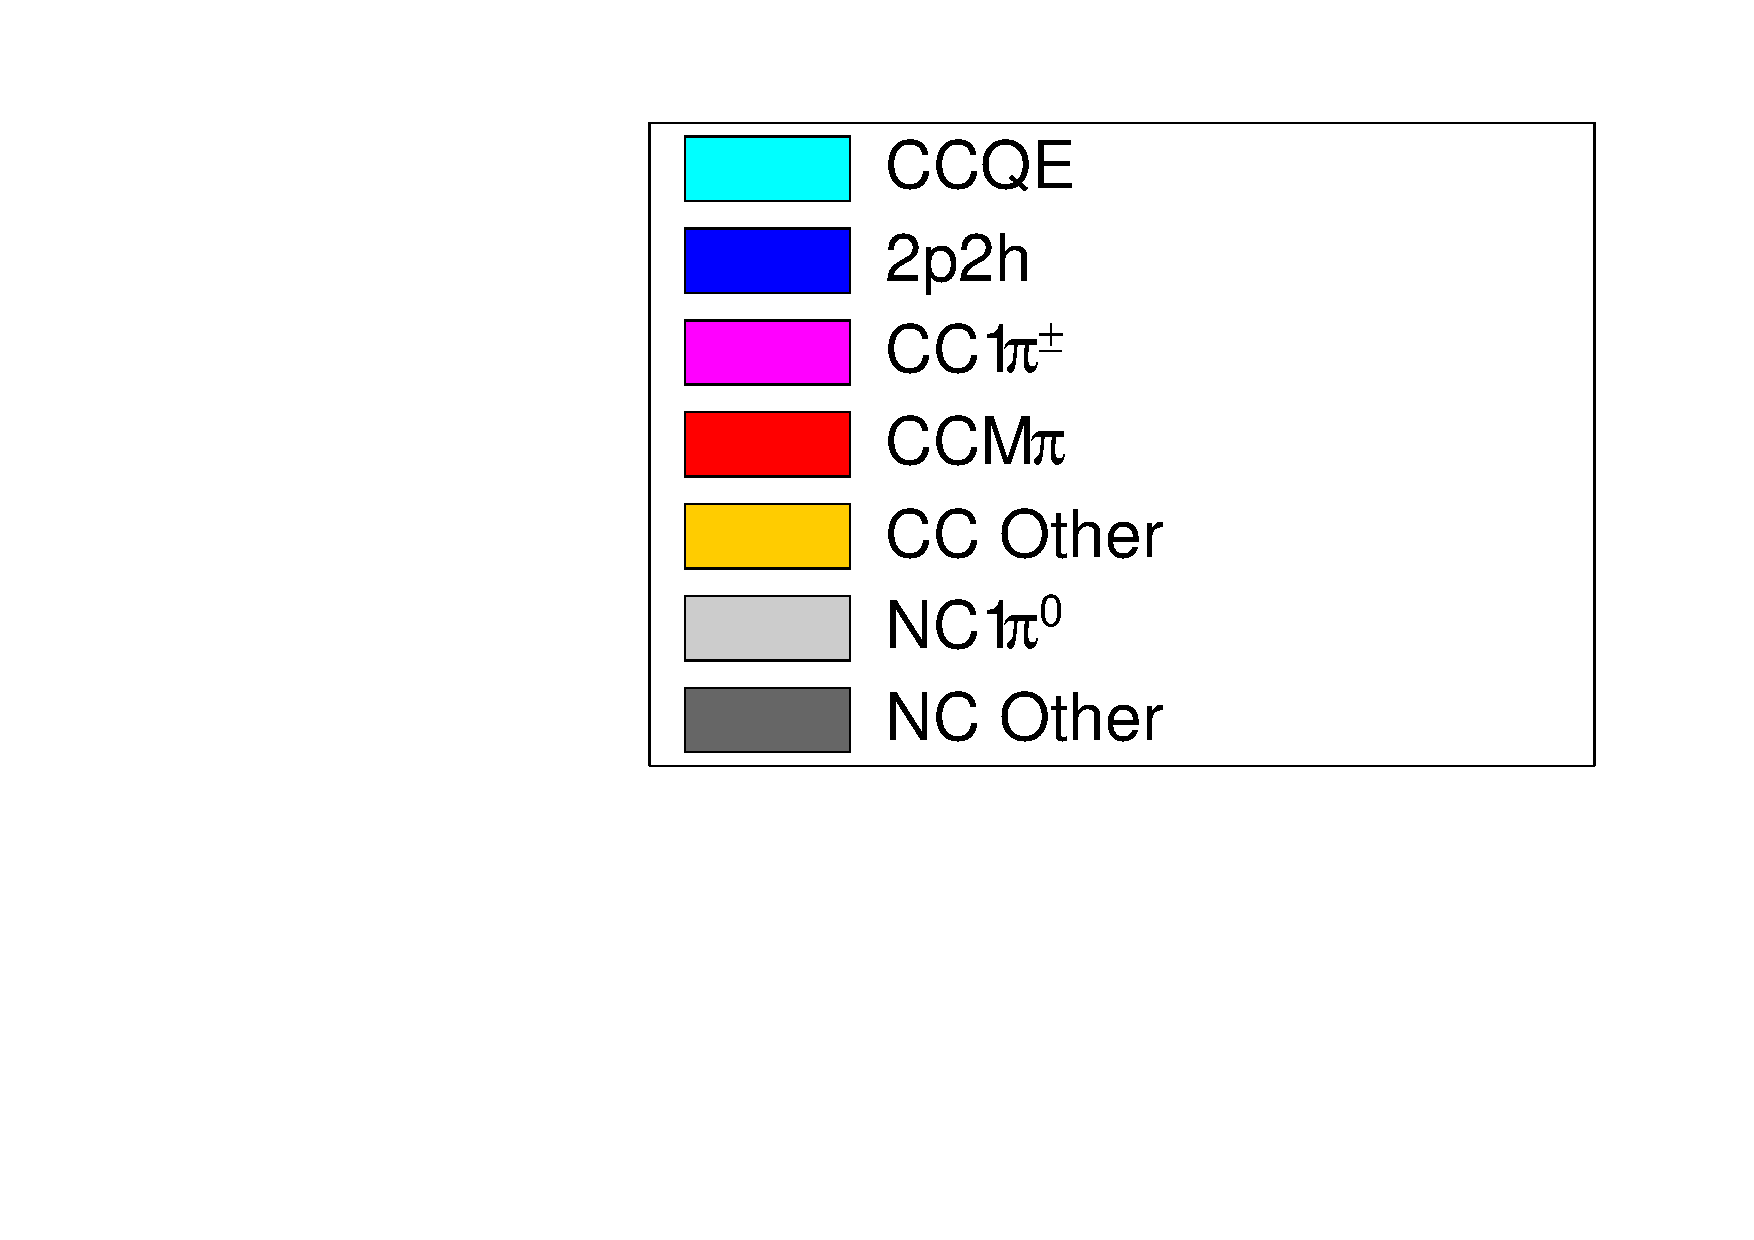
\includegraphics[width=\textwidth, trim={0mm 0mm 0mm 0mm}, clip,page=1]{Figures/Selections/Legend.pdf}
    \subcaption{}
  \end{subfigure}%
  \begin{subfigure}[t]{0.49\textwidth}
    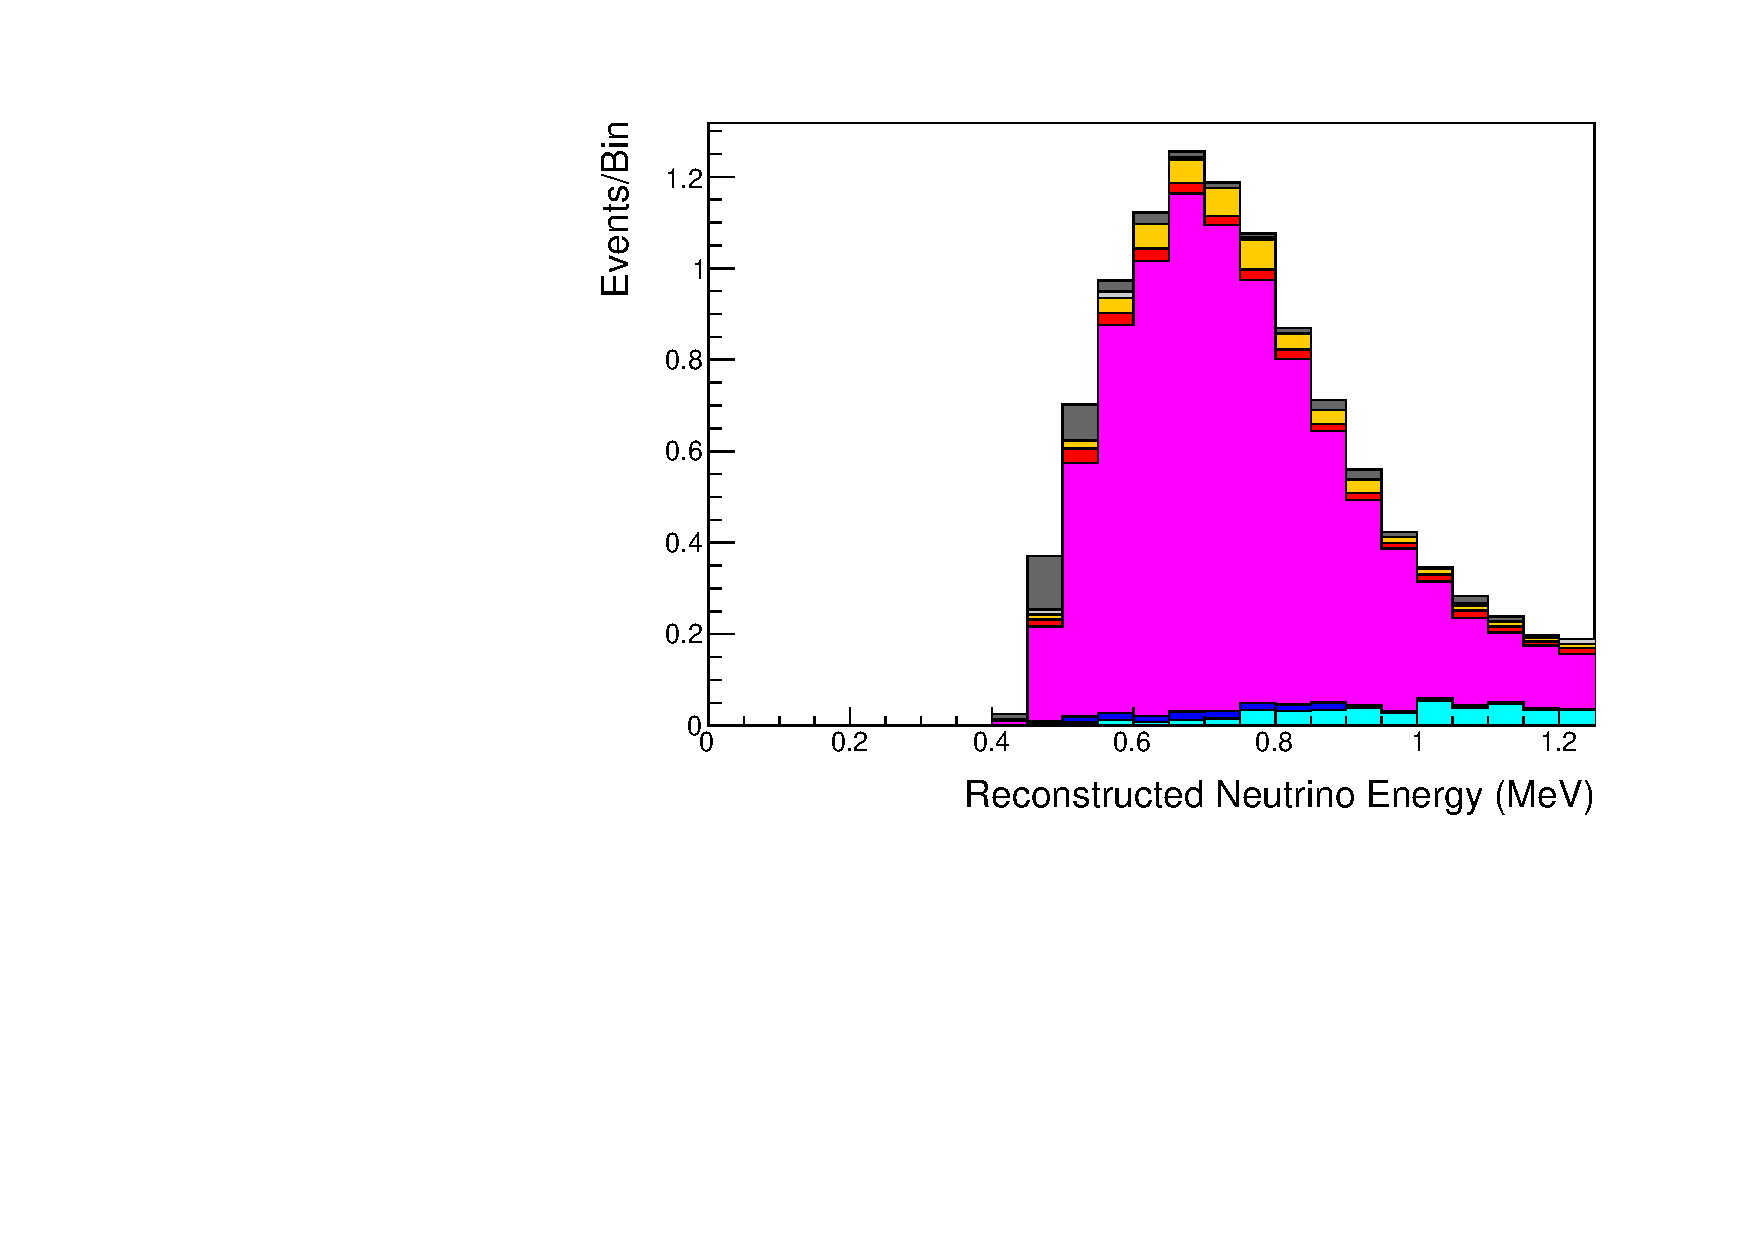
\includegraphics[width=\textwidth, trim={0mm 0mm 0mm 0mm}, clip,page=1]{Figures/Selections/FHCCC1pi-2020_X.pdf}
    \subcaption{FHC CC\quickmath{1\pi^{+}}}
  \end{subfigure}
  \caption{The reconstructed neutrino energy, as defined by \autoref{sec:SelsAndSysts_Erec_CCQE} and \autoref{sec:SelsAndSysts_Erec_CCRES}, for the \quickmath{1\text{R}\mu}, \quickmath{1\text{R}e} and CC\quickmath{1\pi^{+}} samples. The generated dial values and Asimov A oscillation parameter sets are assumed. These samples are the FHC mode samples. For ease of viewing, the \quickmath{1\text{R}\mu} sample only shows the \quickmath{0. \leq E^{rec}_{\nu} < 3.0 \text{GeV}} but the binning extends out to \quickmath{30.0 \text{GeV}}.}
  \label{fig:SelsAndSysts_Beam_ERecSpectra}
\end{figure}

The reconstructed neutrino energy of the CC\quickmath{1\pi^{+}} events is modified to include the delta resonance resonantly produced within the interaction,

\begin{equation}
  \label{sec:SelsAndSysts_Erec_CCRES}
  E^{rec}_{\nu} = \frac{2M_{N}E_{l} + M_{\Delta^{++}}^{2} - M_{N}^{2} - m_{l}^{2}}{2(M_{N} - E_{l} + P_{l}\cos(\theta_{beam}))}
\end{equation}

Where \quickmath{M_{\Delta^{++}}} is the mass of the delta baryon. Binding energy effects are not considered due to the two-body process with the delta baryon is assumed.

The reconstructed neutrino energy for the FHC samples is illustrated in \autoref{fig:SelsAndSysts_Beam_ERecSpectra}. This is the binning used within the analysis. As expected, the \quickmath{1\text{R}\mu} and \quickmath{1\text{R}e} are heavily dominated by CCQE interactions, with smaller contributions from 2p2h meson exchange and resonant pion production interactions. The CC\quickmath{1\pi^{+}} sample predominantly consists of charged current resonant pion production interactions. The \quickmath{1\text{R}e} and CC\quickmath{1\pi^{+}} samples are also binned by the angle between the neutrino beam and the reconstructed lepton momentum. This is to aid in charged current and neutral current separation as indicated in \autoref{fig:SelsAndSysts_Beam_FHC1ReThetaSpectra}. This is because the neutral current backgrounds are predominantly due to \quickmath{\pi^{0}}-decays, where the opening angle of the two gammas alongside the different final state kinematics produces a slightly broader angular distribution compared to the final state particles originating from charged current \quickmath{\nu_{e}} interactions.

\begin{figure}[h]
  \begin{subfigure}[t]{\textwidth}
    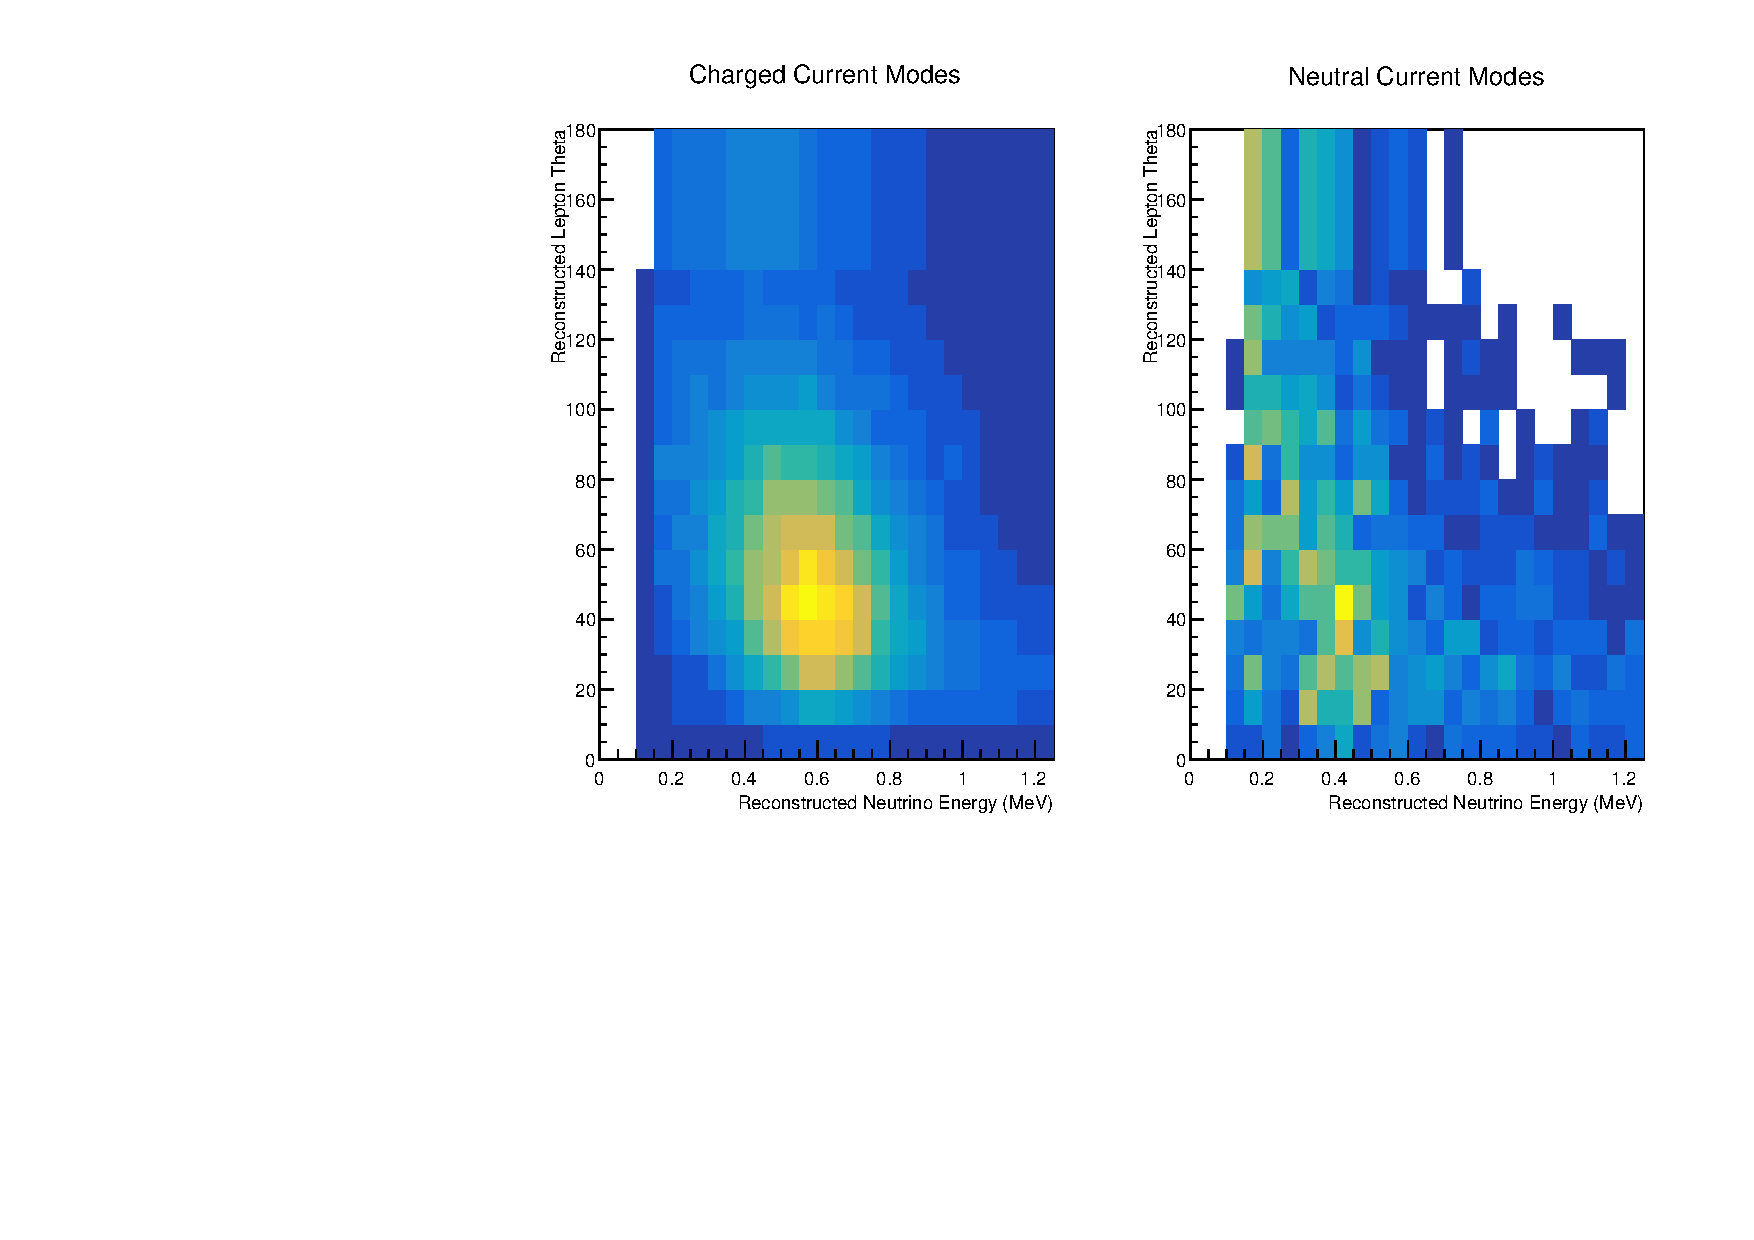
\includegraphics[width=\textwidth, trim={0mm 0mm 0mm 0mm}, clip,page=1]{Figures/Selections/2DSpectra_FHC1Re-2020.pdf}
  \end{subfigure}
  \caption{The distribution of the angle between the neutrino beam direction and the reconstructed final state lepton, for the FHC neutrino mode beam one ring electron sample. The distribution is broken down by neutrino interaction mode into charged current (left) and neutral current (right) components. The pre-fit systematic dial values and Asimov A oscillation parameter sets are assumed.}
  \label{fig:SelsAndSysts_Beam_FHC1ReThetaSpectra}
\end{figure}

\clearpage
\section{Systematic Uncertainties}
\label{sec:SelsAndSysts_Systs}

The systematics for this analysis are split into groups, or blocks, depending on their purpose. They consist of flux uncertainties, neutrino-matter interaction systematics, and detector efficiencies. There are also uncertainties on the oscillation parameters which this analysis will not be sensitive to, \delmsqsol and \sinsqsol. As described in \autoref{chap:MarkovChainMonteCarlo}, each model parameter used within this analysis requires a prior uncertainty. This is provided via separate covariance matrices for each block. The covariance matrices can include prior correlations between parameters within a single block, but the separate treatment means prior uncertainties can not be included for parameters in different groups. Alternatively, some parameters have no reasonably motivated uncertainties. These parameters are assigned flat priors which do not change the likelihood penalty. The flux, neutrino interaction, and detector modeling have already been discussed in \autoref{sec:Simulations_Simulation}. The uncertainties invoked within these models are described below.

\subsection{Beam Flux}
\label{sec:SelsAndSysts_Systs_BeamFlux}

The neutrino beam flux systematics is based upon our uncertainty in the modeling of the components of the beam. This includes the hadron production model and their re-interactions, the shape, intensity, and alignment of the beam with respect to the target, and the uniformity of the magnetic field produced by the horn, alongside other effects. The uncertainty, as a function of neutrino energy, is illustrated in \autoref{fig:SelsAndSysts_BeamFluxSysts} which includes the total uncertainty as well as the individual components. The uncertainty for events below, and much higher than, the peak neutrino energy is dominated by hadron production and re-interaction systematics. The beam profile and alignment of the proton beam dominate the systematic uncertainty for events with \quickmath{E_{\nu} \sim 1\text{GeV}}. 

\begin{figure}[h]
  \begin{subfigure}[t]{\textwidth}
    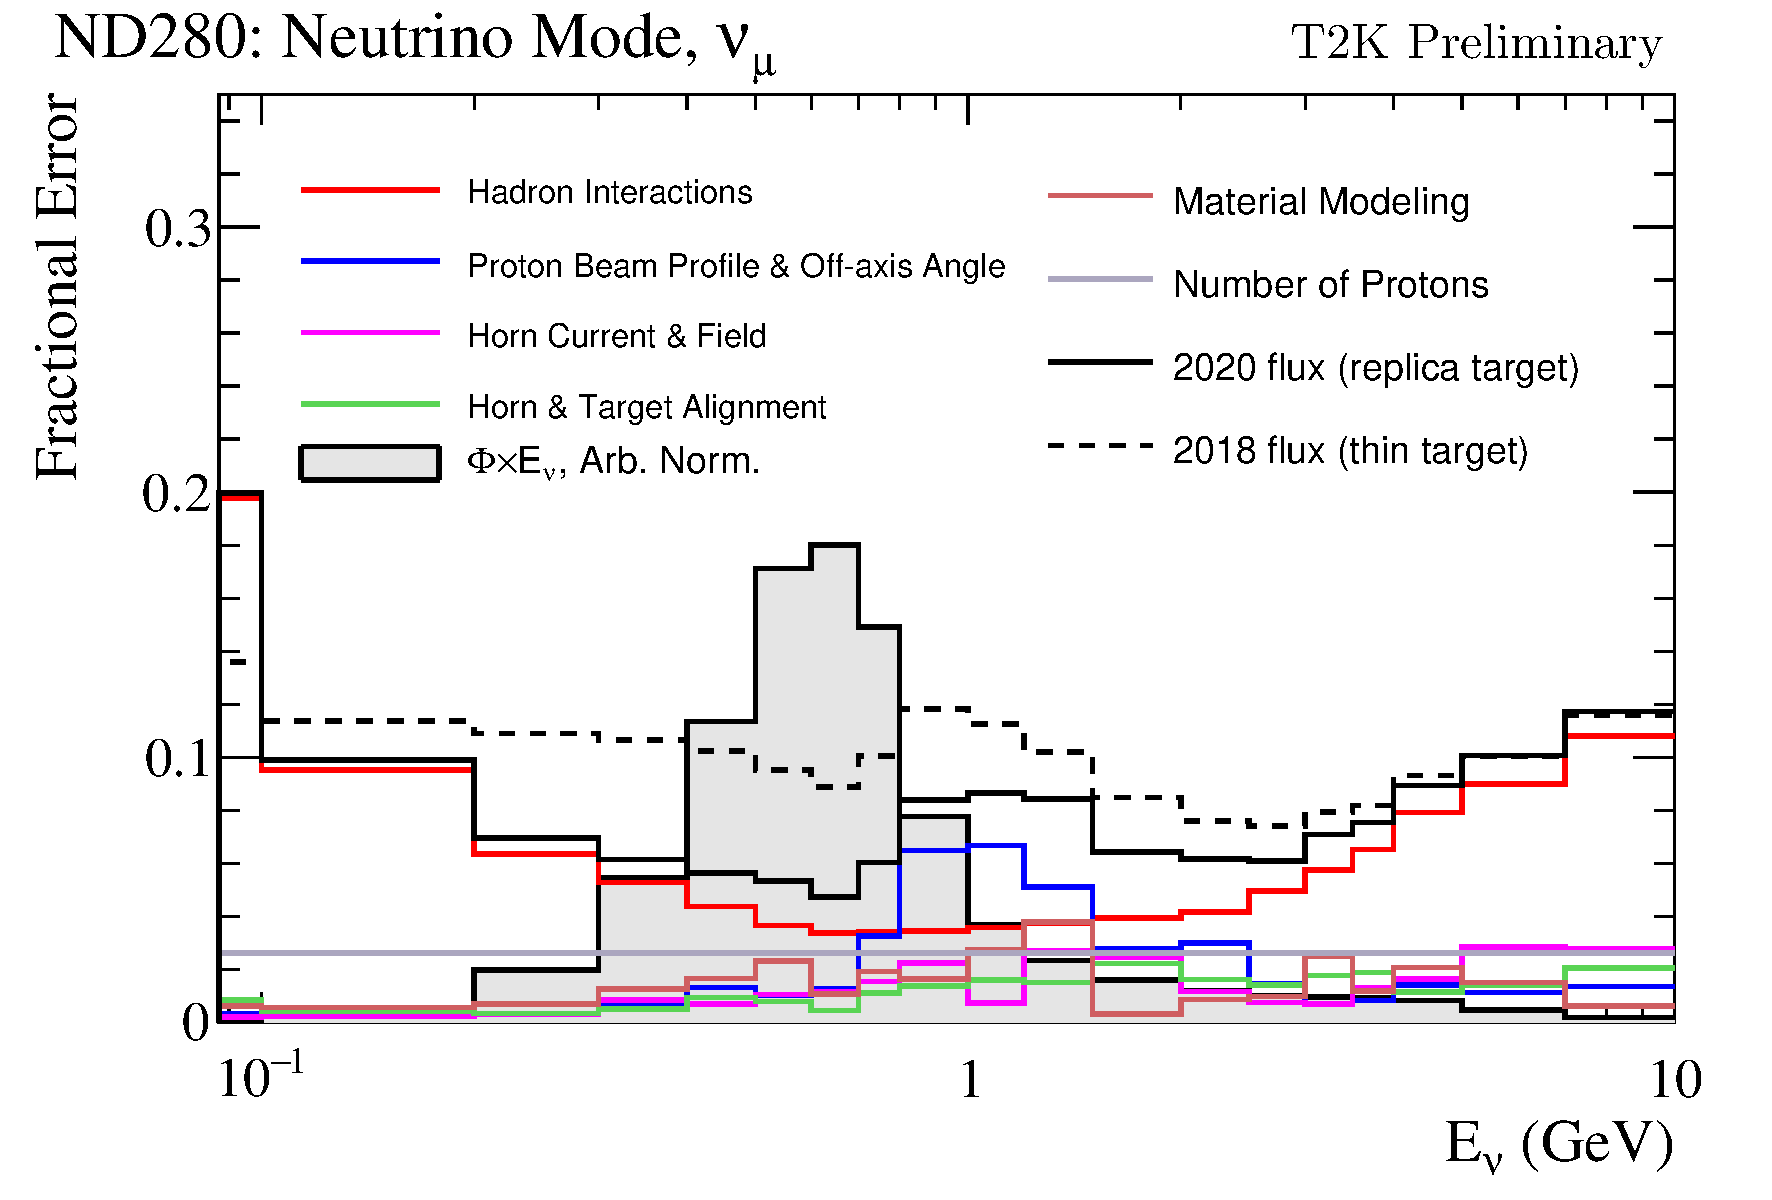
\includegraphics[width=\textwidth, trim={0mm 0mm 0mm 0mm}, clip,page=1]{Figures/Selections/flux_uncertainty_covariance_plots_addcorrnd_compwv3_flux_error_t2k_nd5_fhc_numu.pdf}
  \end{subfigure}
  %\begin{subfigure}[t]{\textwidth}
  %  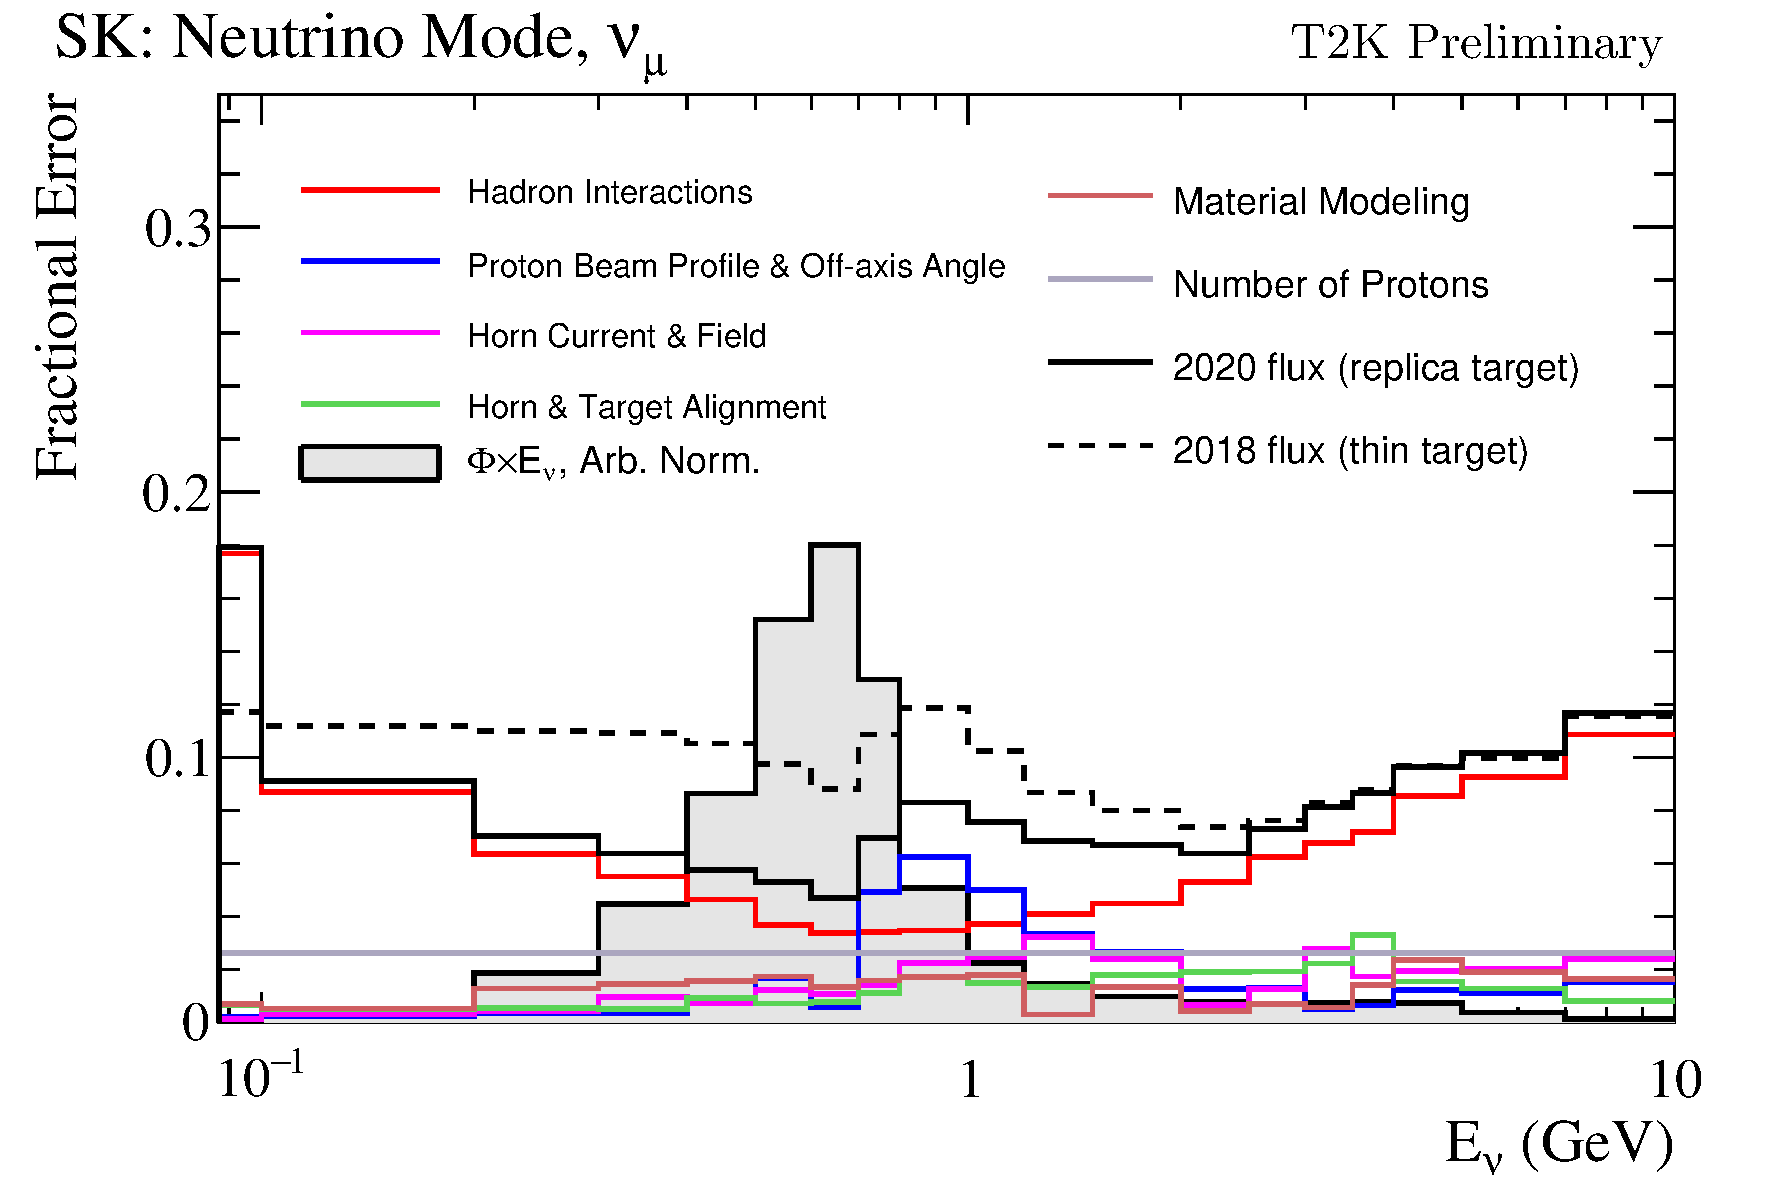
\includegraphics[width=\textwidth, trim={0mm 0mm 0mm 0mm}, clip,page=1]{Figures/Selections/flux_uncertainty_covariance_plots_addcorrnd_compwv3_flux_error_t2k_sk_fhc_numu.pdf}
  %\end{subfigure}
  \caption{The total uncertainty evaluated on the near detector \quickmath{\nu_{\mu}} flux prediction constrained by the replica-target data, illustrated as a function of neutrino energy. The solid(dashed) line indicates the uncertainty used within this analysis(the T2K 2018 analysis). The solid histogram indicates the neutrino flux as a function of energy. Figure taken from \cite{t2k_tn_354}.}
  \label{fig:SelsAndSysts_BeamFluxSysts}
\end{figure}

The beam flux uncertainties are described by one hundred parameters. They are split between both ND280 and SK detectors and binned by neutrino flavour: \quickmath{\nu_{\mu}}, \quickmath{\bar{\nu}_{\mu}}, \quickmath{\nu_{e}} and \quickmath{\bar{\nu}_{e}}. The response is then broken down as a function of neutrino energy. The bin density in the neutrino energy is the same for the FHC-\quickmath{\nu_{\mu}} and RHC-\quickmath{\bar{\nu}_{\mu}}, and narrows for neutrino energies close to the oscillation maxima of \quickmath{E_{\nu} = 0.6\text{GeV}}. This binning is specified in \autoref{tab:SelsAndSysts_BeamFluxBinEdges}. All of these systematic uncertainties are applied as normalisation parameters with Gaussian priors centered at \quickmath{1.0} and error specified from a covariance matrix provided by the T2K beam group.

\begin{table}[ht!]
    \centering
    \begin{tabular}{c|c|c}
      \hline
      Neutrino Flavour & Sign & Neutrino Energy Bin Edges (GeV) \\
      \hline
      \quickmath{\mu} & Right & \quickmath{0.,0.4,0.5,0.6,0.7,1.,1.5,2.5,3.5,5.,7.,30.} \\
      \quickmath{\mu} & Wrong & \quickmath{0.,0.7,1.,1.5,2.5,30.} \\
      \quickmath{e} & Right & \quickmath{0.,0.5,0.7,0.8,1.5,2.5,4.,30.} \\
      \quickmath{e} & Wrong & \quickmath{0.,2.5,30.} \\
      \hline
      \hline
    \end{tabular}
    \caption{The neutrino energy binning for the different neutrino flavours. ``Right'' sign indicates neutrinos in the FHC beam and antineutrinos in the RHC beam mode. ``Wrong'' sign indicates antineutrinos in the FHC beam and neutrinos in the RHC beam mode. The binning of the detector response is identical for the FHC and RHC modes as well as at ND280 and SK.}
    \label{tab:SelsAndSysts_BeamFluxBinEdges}
\end{table}

\subsection{Atmospheric Flux}
\label{sec:SelsAndSysts_Systs_AtmFlux}
The atmospheric neutrino flux is modeled by the HKKM model, however, 16 systematic uncertainties are applied to control the normalisation of each neutrino flavour, energy, and direction. All of the parameters are given Gaussian priors centered at \quickmath{0} and width \quickmath{1.}. They are summarised below:

\begin{itemize}
\item \textbf{Absolute Normalisation}: The overall normalisation of each neutrino flavour is controlled by two independent systematic uncertainties, for \quickmath{E_{\nu} < 1\text{GeV}} and \quickmath{E_{\nu} > 1\text{GeV}}, respectively. This is driven mostly by hadronic interaction uncertainties for the production of pions and kaons \cite{Honda_2007}. The strength of the response is dependent upon the neutrino energy.
\item \textbf{Relative Normalisation}: Uncertainties on the ratio of \quickmath{(\nu_{\mu} + \bar{\nu}_{\mu})/(\nu_{e} + \bar{\nu}_{e})} are controlled by the difference between the HKKM model \cite{Honda_2007}, FLUKA \cite{etde_20239111} and Bartol models \cite{Barr_2004}. Three independent parameters are applied in the energy ranges: \quickmath{E_{\nu} < 1\text{GeV}}, \quickmath{1\text{GeV} < E_{\nu} < 10 \text{GeV}}, and \quickmath{E_{\nu} > 10\text{GeV}}.
\item \textbf{\quickmath{\nu}/\quickmath{\bar{\nu}} Normalisation}: The uncertainties in the \quickmath{\pi^{+}/\pi^{-}} (and kaon equivalent) produce uncertainties in the flux of \quickmath{\nu/\bar{\nu}}. The response is applied in the same way as the relative normalisation parameters.
\item \textbf{Up/Down and Vertical/Horizontal Ratio}: Similar to the above two systematics, the difference between the HKKM, FLUKA, and Bartol model predictions, as a function of \quickmath{\cos(\theta_{Z})}, is used to control the normalisation of events as a function of zenith angle.
\item{\textbf{\quickmath{K/\pi} Ratio}}: Higher energy neutrinos (\quickmath{E_{\nu} < 10\text{GeV}}) become dependent upon kaon decay as the dominant source of neutrinos. Measurements of the ratio of \quickmath{K/\pi} \cite{Ambrosini1998-er} are used to control the systematic uncertainty of the expected ratio of pion and kaon production.
\item \textbf{Solar Activity}: As the 11-year solar cycle can affect the Earth's magnetic field, the flux of primary cosmic rays is modulated across the same period. The uncertainty is calculated by taking a \quickmath{\pm 1} year variation, equating to a \quickmath{10\%} uncertainty for the SK-IV period.
\item \textbf{Atmospheric Density}: The height of the interaction of the primary cosmic rays is dependent upon the atmospheric density. The HKKM assumes the US standard 1976 \cite{USStandardAtm} profile. This systematic controls the uncertainty in that model.
\end{itemize}

Updates to the HKKM and Bartol models are underway to use a similar tuning technique to that used in the beam flux predictions. After those updates, it may be possible to include correlations in the hadron production uncertainty systematics for beam and atmospheric flux predictions.

\subsection{Neutrino Interaction}
\label{sec:SelsAndSysts_Systs_Interaction}

The neutrino interactions which occur within all the detectors are modeled by NEUT. The two independent oscillation analyses, T2K beam only and the SK atmospheric only, have developed separate interaction models. The T2K-only analysis uses the systematics model defined in \cite{t2k_tn_344} and the SK-only analysis uses the uncertainties detailed in \cite{Kamiokande_Collaboration2017-nf}. To leverage the most sensitivity out of this joint beam and atmospheric analysis, a correlated interaction model has been defined. Where applicable, these correlations allow the systematic uncertainties applied to the atmospheric samples to be constrained by measurements of the near detector in the beam experiment leading to stronger sensitivity to oscillation parameters as compared to an uncorrelated model. An in-depth discussion of the reasoning and validity of enforcing correlations is documented in \cite{t2k_tn_422} and briefly summarised below.

The low energy T2K systematic model has a more sophisticated treatment of CCQE, CCMEC, and CCRES uncertainties which is due to the purpose-made cross-section measurements made by the near detector. Furthermore, extensive testing of this model has been performed by the working group responsible for this model \cite{t2k_tn_344}. However, it is not designed for the high-energy atmospheric events illustrated in \autoref{fig:Simulations_NeutrinoEnergyDistribution}. Therefore the high energy systematic model from the SK-only analysis is implemented for the relevant multiGeV samples. The CCQE systematic parameters invoked within the SK high energy model are actually contained within T2K's CCQE model. Consequently, the more sophisticated CCQE and CCMEC T2K model parameters have been incorporated into the high energy model but are uncorrelated from the low energy counterparts. This results in a more complete model but without any constraint from the near detector measurements.

The high energy systematic model includes parameters developed from comparisons of Nieves and Rein-Seghal models which affect CCRES interactions, comparisons of the GRV98 and CKMT models which control DIS interactions, and hadron multiplicity measurements which modulate the normalisation of CC\quickmath{N\pi} events. The uncertainty of the \quickmath{\nu_{\tau}} cross-section is particularly large and is controlled by a \quickmath{25\%} normalisation uncertainty. These parameters are applied via normalisation or shape parameters. The former linearly scales the weight of all affected Monte-Carlo events, whereas the latter can increase or decrease a particular event's weight depending on its neutrino energy and mode of interaction. The response of the shape parameters are defined by third-order polynomial splines which return a weight for a particular neutrino energy. In total, \quickmath{17} normalisation and \quickmath{15} shape parameters are included in the more sophisticated high-energy model.

\autoref{fig:SelsAndSysts_NeutrinoEnergyComparison} indicates the predicted neutrino energy distribution for both beam and subGeV atmospheric samples, and \autoref{fig:SelsAndSysts_FractionalModeComparison} illustrates the fractional contribution of the different interaction modes per sample. There is clearly significant overlap in neutrino energy between the subGeV atmospheric and beam samples, allowing similar kinematics in the final state particles. Comparing beam samples with zero decay electrons and atmospheric electron-like(muon-like) samples with zero(zero or one) decay electrons, there is a very similar contribution of CCQE, CC 2p2h, and CC\quickmath{1\pi^{\pm}} interactions. The samples which target CC\quickmath{1\pi^{\pm}} interactions, FHC 1R\quickmath{e}1de beam sample and atmospheric electron-like(muon-like) samples with one(two) decay electrons, also consist of very similar mode interactions. As a consequence of the similarity in energy and mode contributions, correlating the systematic model between the beam and subGeV atmospheric samples ensures that this analysis attains the largest sensitivity to oscillation parameters while still ensuring neutrino interaction systematics are correctly accounted for. Due to its sophisticated CCQE model, the T2K systematic model was chosen as the basis of the correlated model. 

\begin{figure}[h]
  \begin{subfigure}[t]{0.49\textwidth}
    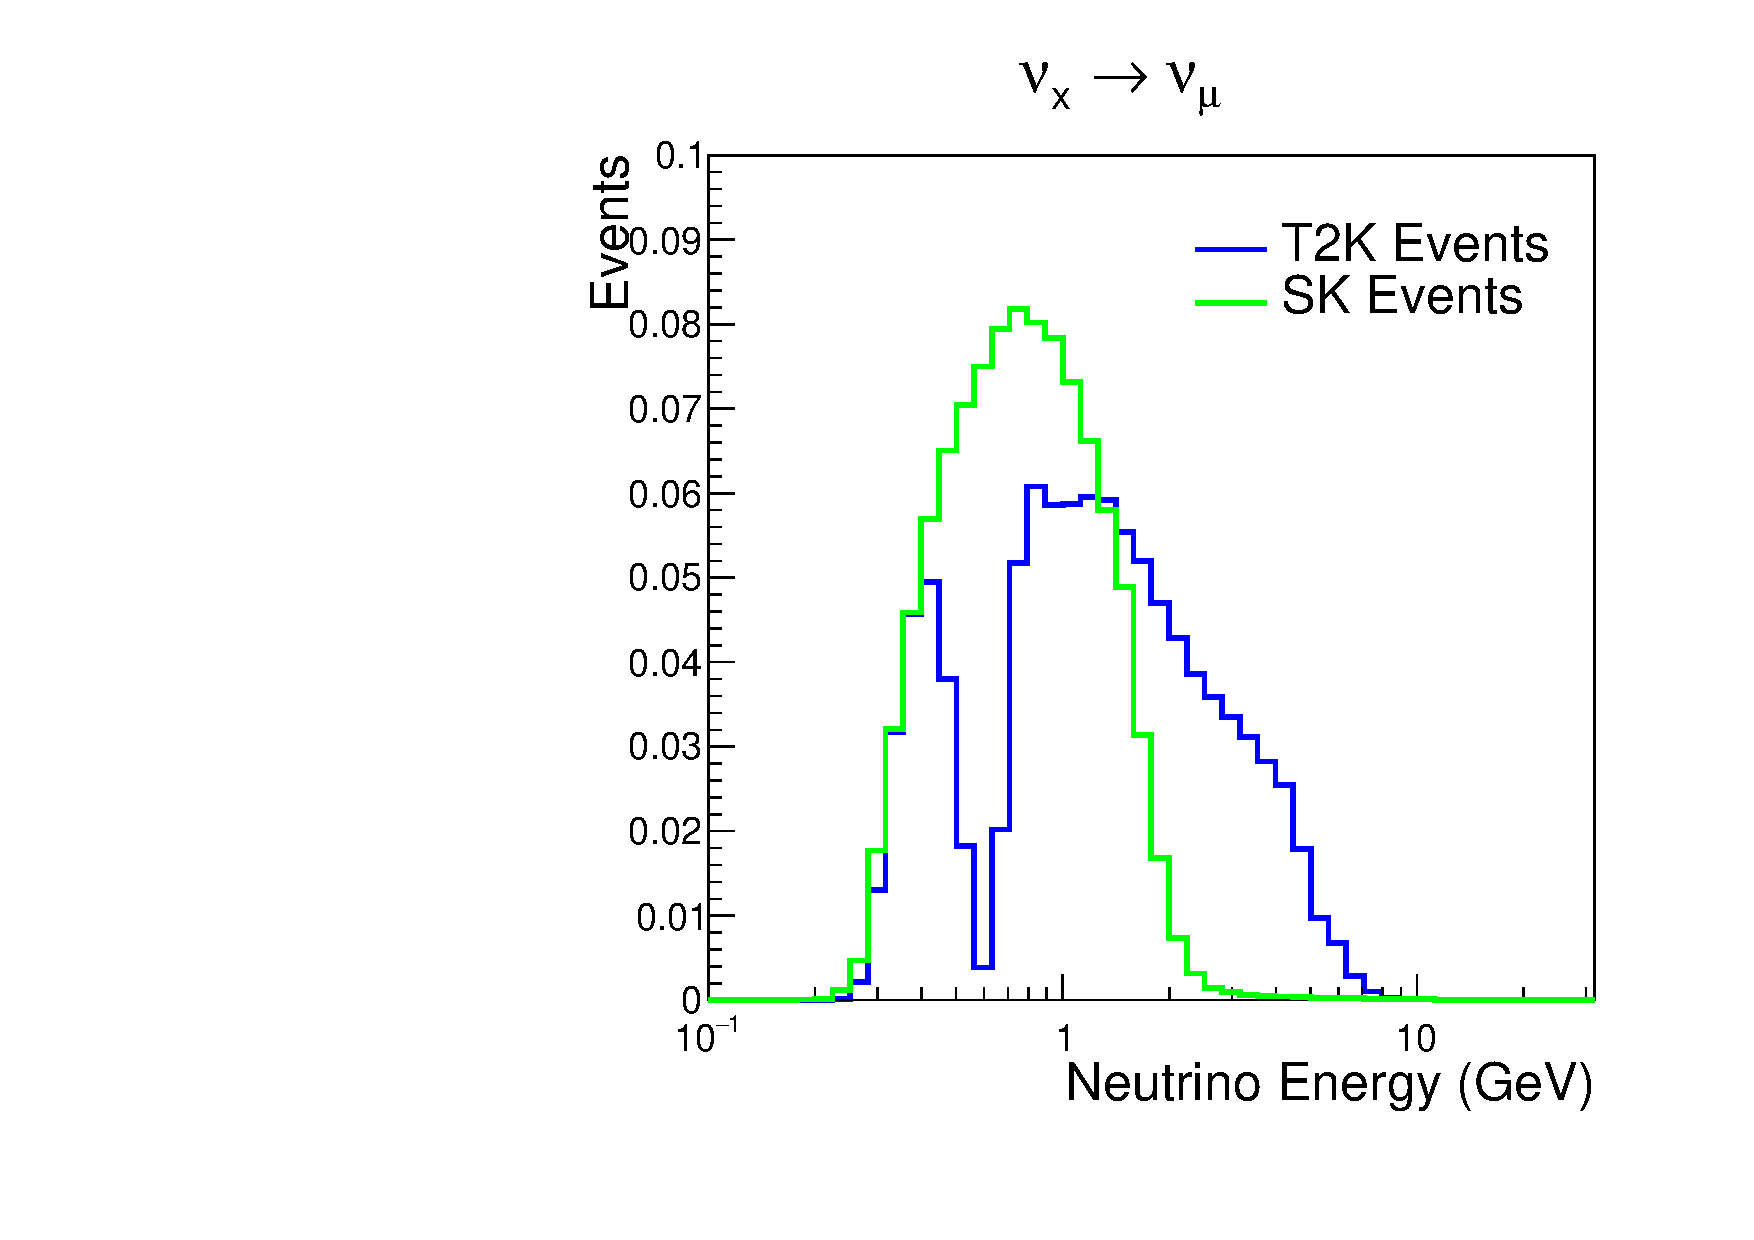
\includegraphics[width=\textwidth, trim={0mm 0mm 0mm 0mm}, clip,page=1]{Figures/Selections/NeutrinoEnergyDist_Comp_1Rmu_NuMu.pdf}
    \subcaption{\quickmath{\mu}-like}
  \end{subfigure}%
  \begin{subfigure}[t]{0.49\textwidth}
    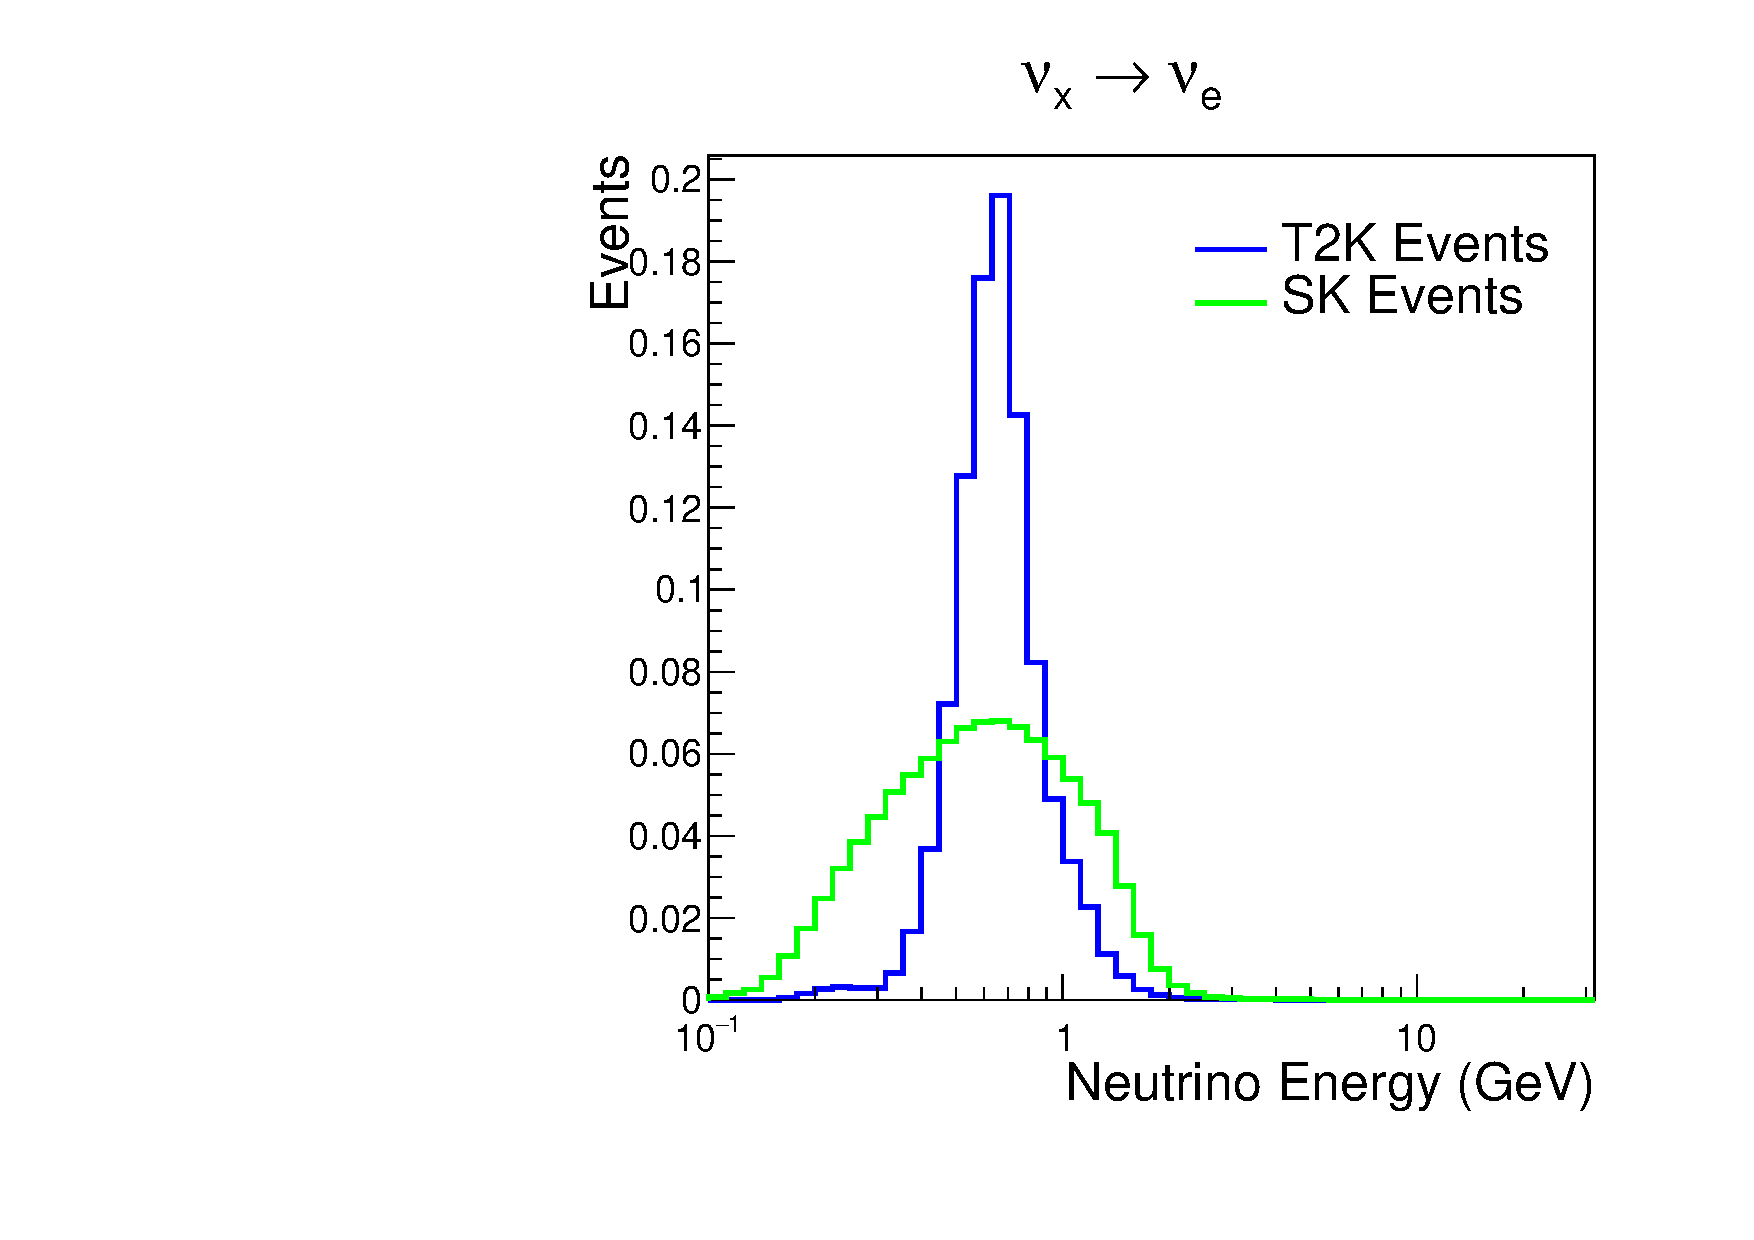
\includegraphics[width=\textwidth, trim={0mm 0mm 0mm 0mm}, clip,page=1]{Figures/Selections/NeutrinoEnergyDist_Comp_1Re_NuE.pdf}
    \subcaption{\quickmath{e}-like}
  \end{subfigure}
  \begin{subfigure}[t]{0.49\textwidth}
    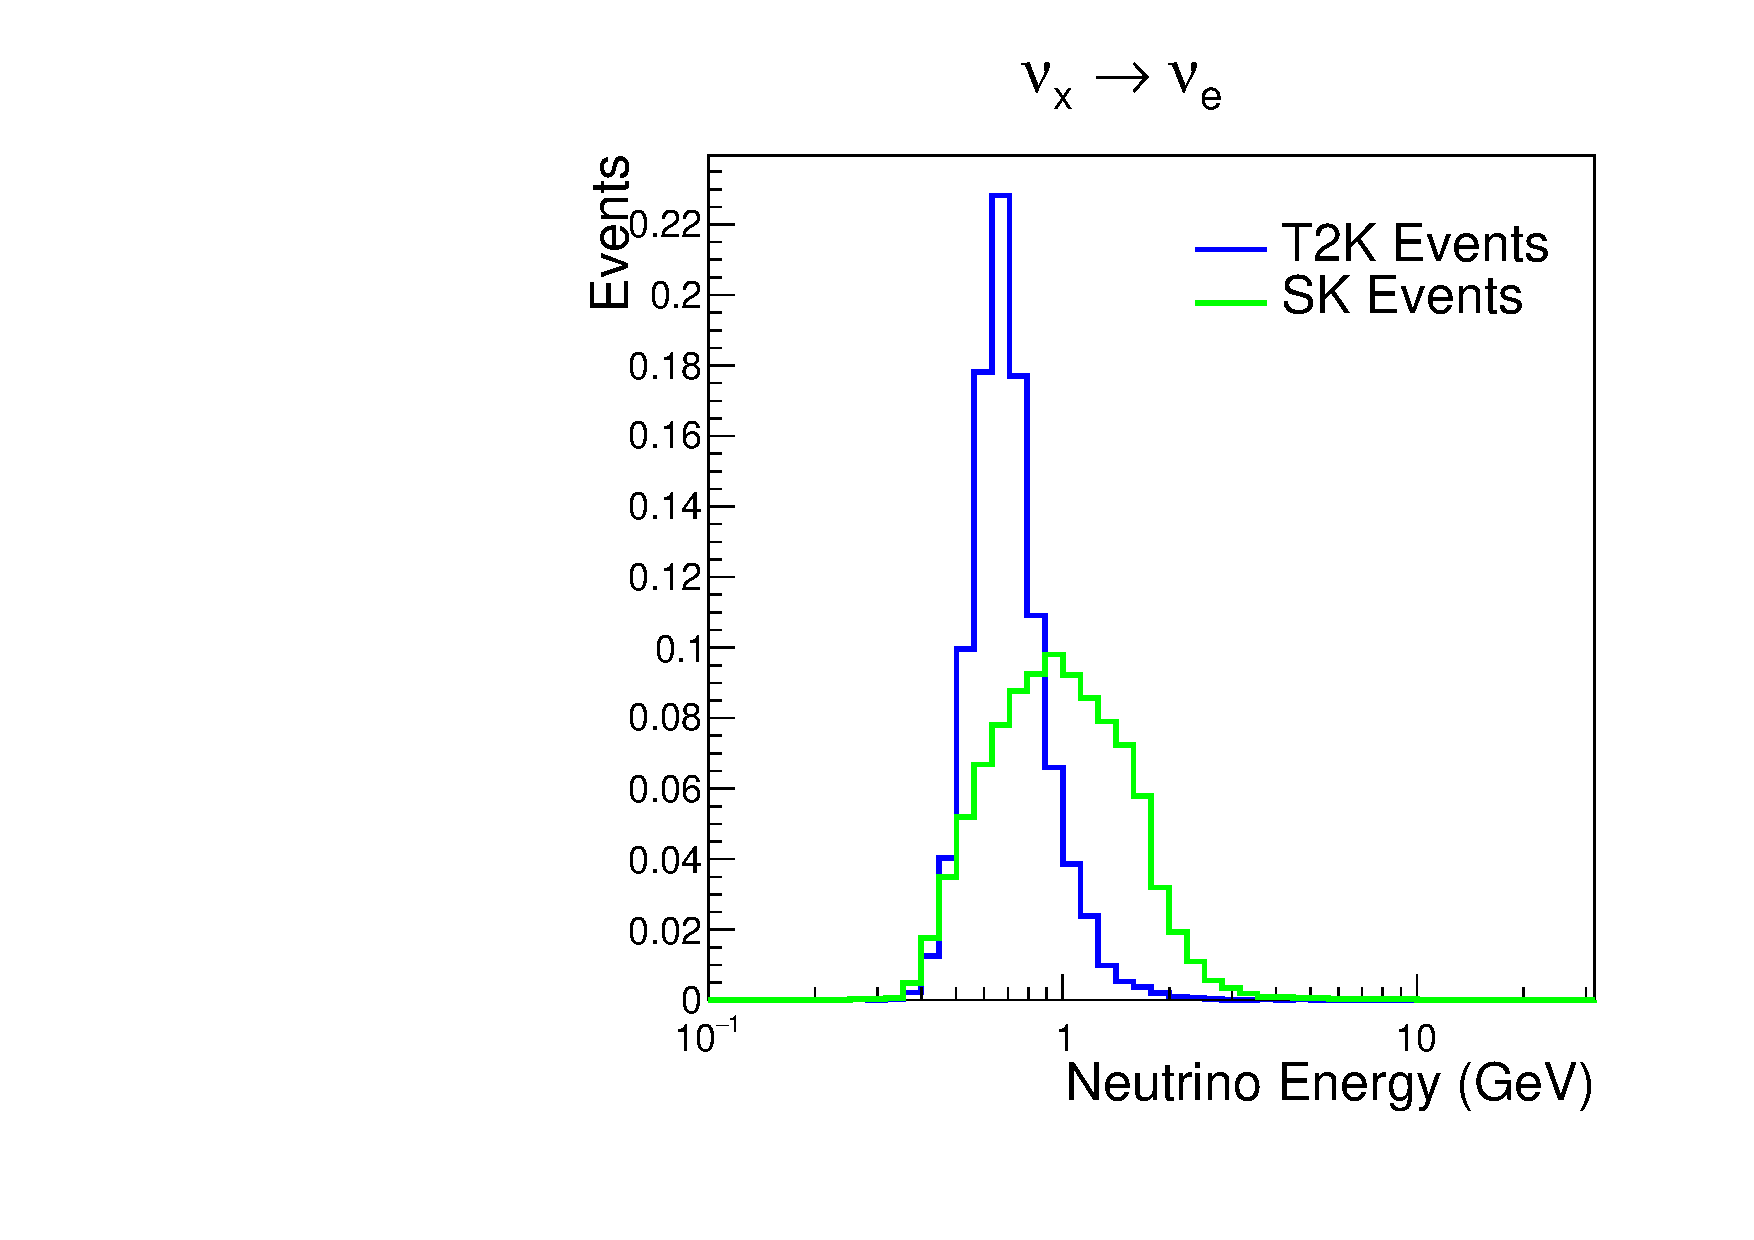
\includegraphics[width=\textwidth, trim={0mm 0mm 0mm 0mm}, clip,page=1]{Figures/Selections/NeutrinoEnergyDist_Comp_1Re1de_NuE.pdf}
    \subcaption{\quickmath{e}-like + 1d.e.}
  \end{subfigure}
  \caption{The prediction neutrino energy distribution for subGeV atmospheric and beam samples, given for muon-like samples FHC+RHC 1R\quickmath{\mu} beam samples compared to the subGeV \quickmath{\mu}-like 0+1 decay electrons (d.e.) atmospheric samples, electron-like 0d.e. samples FHC+RHC 1R\quickmath{e} beam samples compared to the subGeV \quickmath{e}-like 1d.e. sample, and electron-like 1d.e. sample FHC1Re1de beam sample compared to the subGeV \quickmath{e}-like 1d.e. atmospheric sample.}
  \label{fig:SelsAndSysts_NeutrinoEnergyComparison}
\end{figure}

\begin{figure}[h]
  \begin{subfigure}[t]{\textwidth}
    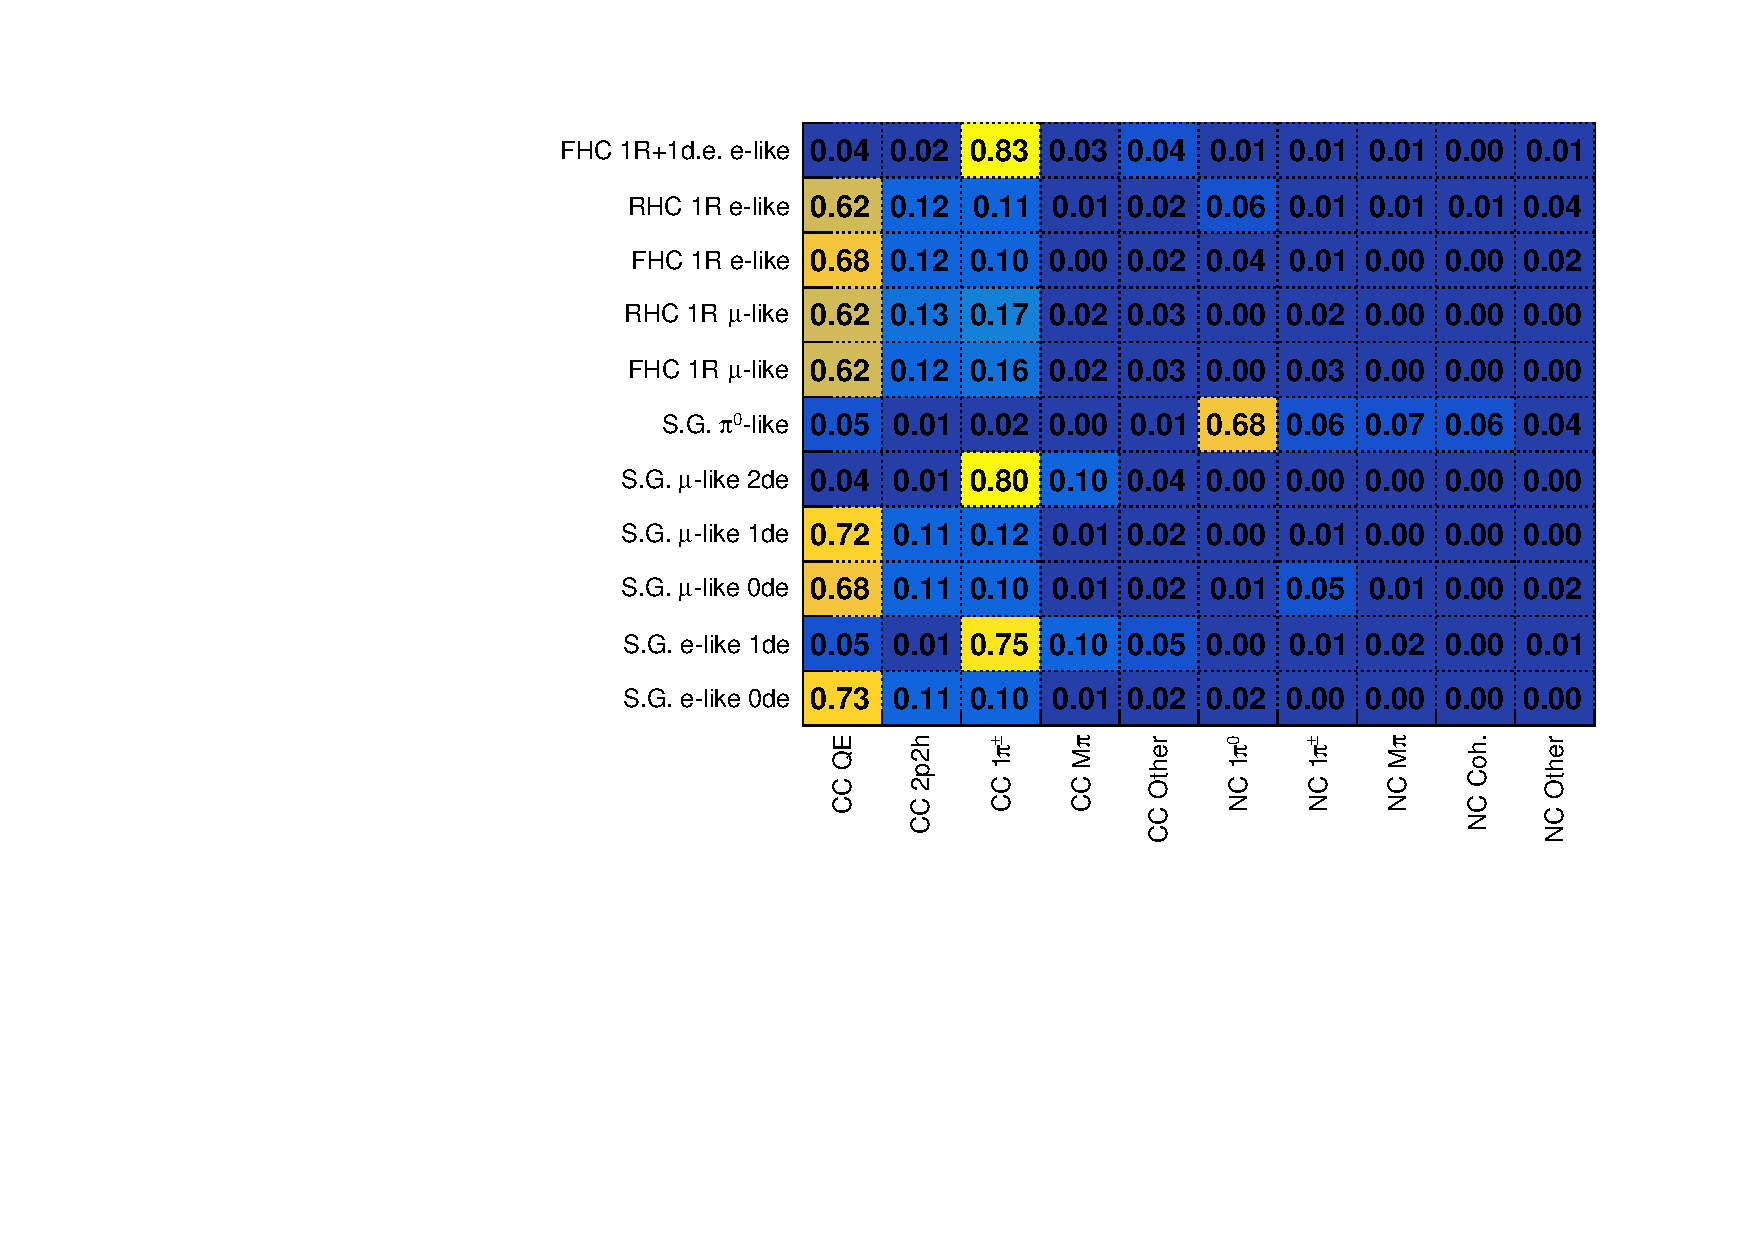
\includegraphics[width=\textwidth, trim={0mm 0mm 0mm 0mm}, clip,page=1]{Figures/Selections/FractionalModeComparison.pdf}
  \end{subfigure}
  \caption{The interaction mode contribution of each sample given as a fraction of the total event rate in that sample. All systematic dials are set to their nominal values and the Asimov A oscillation parameters are assumed. The Charged Current (CC) modes are broken into quasi-elastic (QE), meson exchange (2p2h), resonant charged pion production (\quickmath{1\pi^{\pm}}), multi-pion production (\quickmath{M\pi}), and other interaction categories. Neutral Current (NC) interaction modes are given in interaction mode categories: \quickmath{\pi^{0}} production, resonant charged pion production,  multi-pion production, and others.}
  \label{fig:SelsAndSysts_FractionalModeComparison}
\end{figure}

The T2K uncertainty model is applied in a similar methodology to the SK model parameters. It consists of \quickmath{19} shape parameters applied via third-order polynomial splines and \quickmath{24} normalisation parameters. Four additional parameters, which model the uncertainty in the binding energy, are applied in a way to shift the momentum of the lepton emitted from a nucleus. The majority of these parameters are assigned a Gaussian prior uncertainty. Those that have no theoretical reasoning, or those which have not been fit to external data, are assigned a flat prior which does not affect the penalty term. The CCQE model parameters were tuned to MiniBooNE \cite{miniboone_nu_ccqe} and MINER\quickmath{\nu}A \cite{minerva_nubar_ccqe} measurements and CCRES model parameters are tuned to ANL and BNL experiments \cite{ANL_BNL_corr}.

There are three particular tunes of the T2K low energy cross section model typically considered. Firstly, the ``generated'' tune which is the set of dial values with which the Monte Carlo was generated. Secondly, the set of dial values which are taken from external data measurements and used as inputs. These are the ``pre-fit'' dial values. The reason these two sets of dial values are different is that the external data measurements are continually updated but it is very computationally intensive to regenerate a Monte Carlo prediction after each update. Consequently, the pre-fit and generated dial values differ. The final tune is the ``post-fit'' or ``post-BANFF'' dial values. These are the values taken from a fit to the beam near detector data. This fit is performed by two independent fitting frameworks, \texttt{MaCh3} and \texttt{BANFF}, which ensures reliable measurements. The output of each fitter is converted into a covariance matrix to describe the error and correlations between all the cross-section parameters. This is then propagated to the far-detector oscillation analysis group for use in the \texttt{P-Theta} fitting framework. As \text{MaCh3} can perform a near detector fit, it is included within the simultaneous fit of the far-detector beam and atmospheric oscillation analysis. This is because this technique does not require any assumption of Gaussian posterior distributions which is required in the covariance matrix methodology.

On top of the combination of the SK and T2K interaction models, several other parameters have been specifically developed for the joint oscillation analysis. As the majority of the atmospheric samples' \dcp sensitivity comes from the normalisation of subGeV electron-like events, an additional dial that models an alternative Continous Random Phase Approximation (CRPA) nuclear ground state has been implemented \cite{t2k_tn_422}. As the near detector can not sufficiently constrain the model, this dial approximates the event weights if a CRPA model had been assumed rather than a spectral function. This dial only effects \quickmath{\nu_{e}} and \quickmath{\bar{\nu}_{e}} and is applied as a shape parameter.

Further additions to the model have been included due to the subGeV \quickmath{\pi^{0}} atmospheric sample. This particularly targets charged current and neutral current \quickmath{\pi^{0}} producing interactions to constrain the systematic uncertainties. However, there is no analogous sample in the T2K beam-only analysis so no significant effort has been placed into building a sufficient uncertainty model. Therefore, an uncertainty that affects neutral current resonant \quickmath{\pi^{0}} production is incorporated in this analysis. Comparisons of NEUT's NC resonant pion production predictions have been made to MiniBooNE \cite{MB_NC1pi0} data and a consistent \quickmath{16\%} to \quickmath{21\%} underprediction is observed. Consequently, a conservative \quickmath{30\%} normalisation is invoked. 

Events which originate from above the detector and travel downward are very insensitive to oscillation parameters and act similar to the near detector within an accelerator experiment (Details are illustrated in \autoref{chap:OscillationProbability}). Consequently, the application of the T2K low energy cross section and the effect of the near detector constraint on the atmospheric samples can be studied through these events, without biasing the results from oscillation effects. The downward going predictives are illustrated in \autoref{fig:SelsAndSysts_DownGoingPredictives}. For samples that target CCQE interactions (electron-like with 0 decay electrons and muon-like with 0 or 1 decay electrons), the application of the near detector constraint is well within statistical fluctuation of the down-going data and no significant tension is observed between the data and the Monte Carlo prediction with the T2K near detector constraint. This is not the case for samples with target CCRES interactions (electron-like with 1 decay electron and muon-like with 2 decay electrons). The electron-like data is consistent with the constrained prediction at higher reconstructed momenta but diverges at lower momentum, whereas the muon-like sample is under-predicted throughout the range of momenta. To combat this disagreement, an additional cross-section systematic dial, specifically designed to inflate the low pion momentum systematics was developed in \cite{t2k_tn_422}. This is a shape parameter implemented through a splined response.

\begin{figure}[h]
  \begin{subfigure}[t]{0.49\textwidth}
    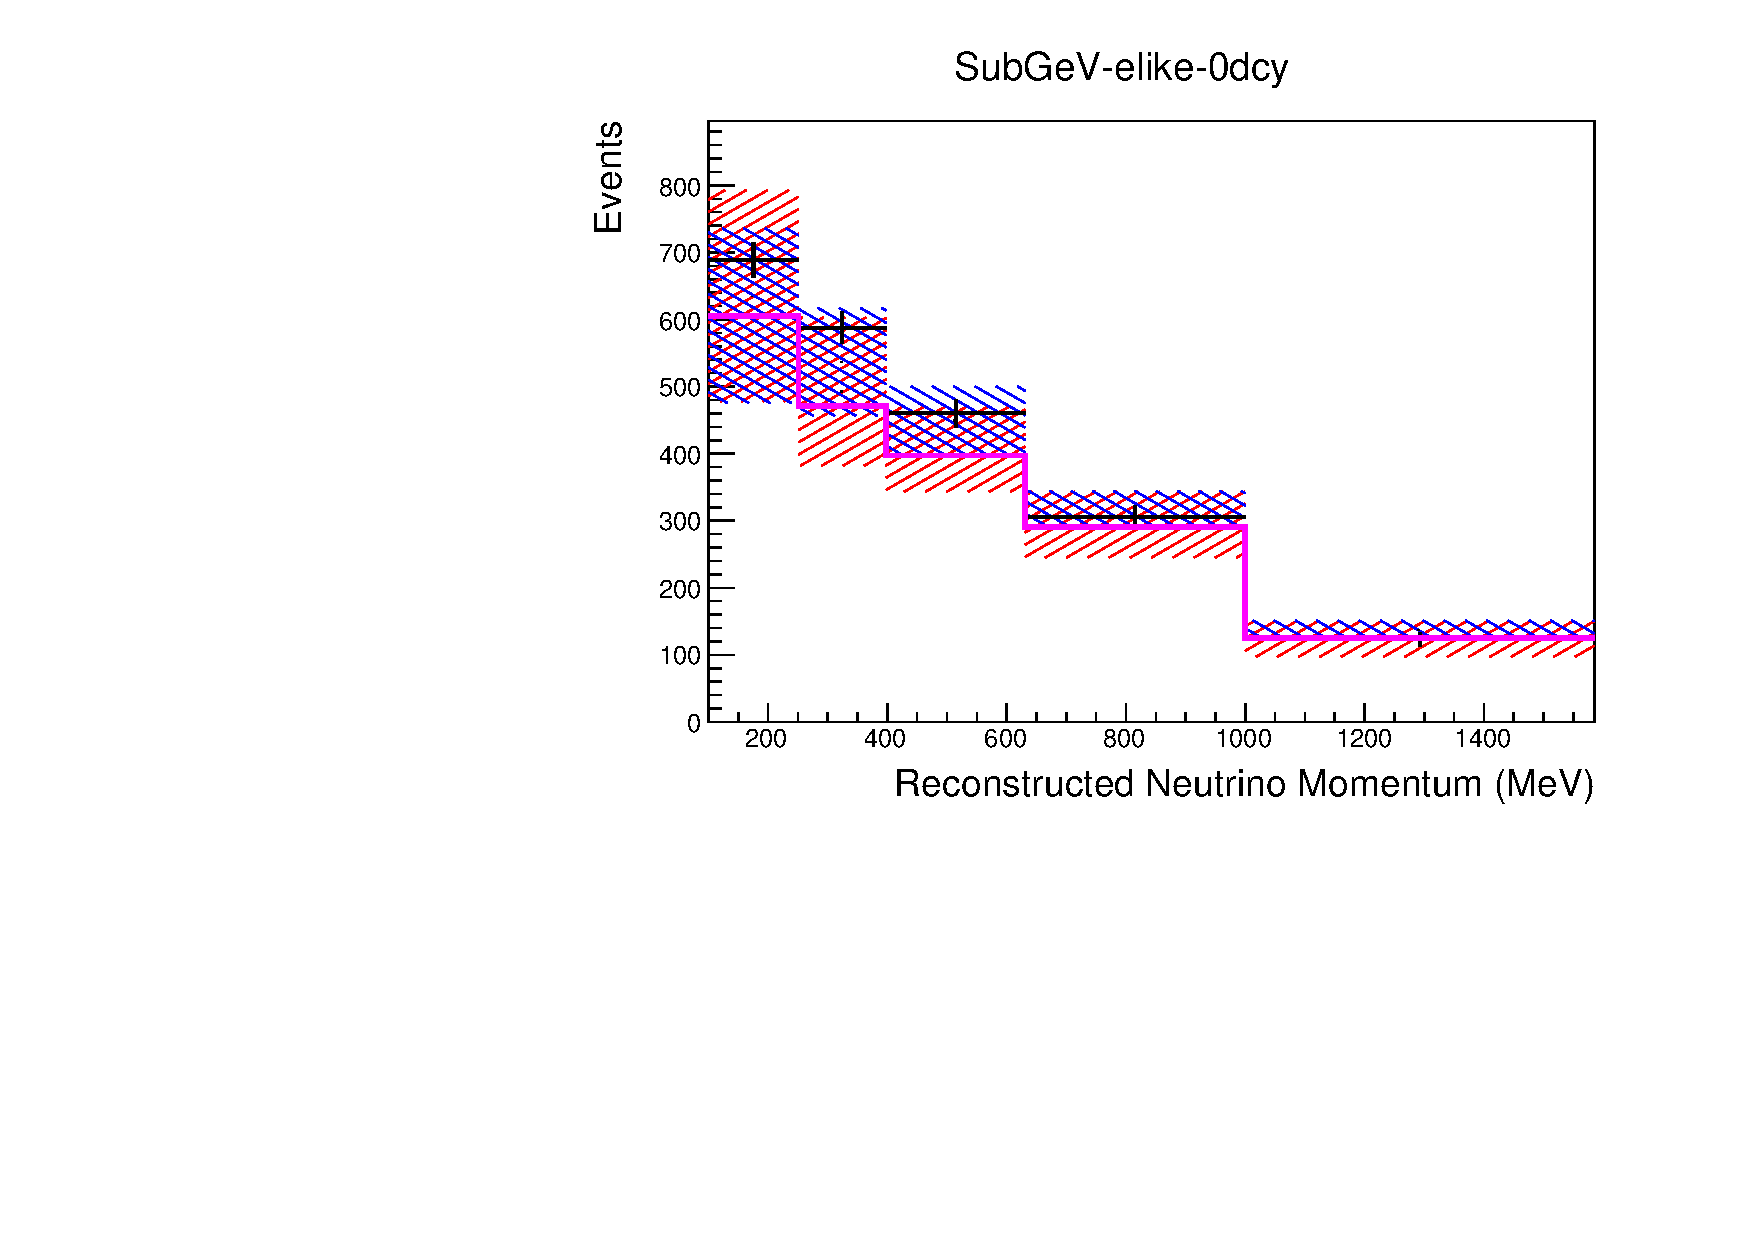
\includegraphics[width=\textwidth, trim={0mm 0mm 0mm 0mm}, clip,page=1]{Figures/Selections/Predictive_SubGeV-elike-0dcy.pdf}
  \end{subfigure}%
  \begin{subfigure}[t]{0.49\textwidth}
    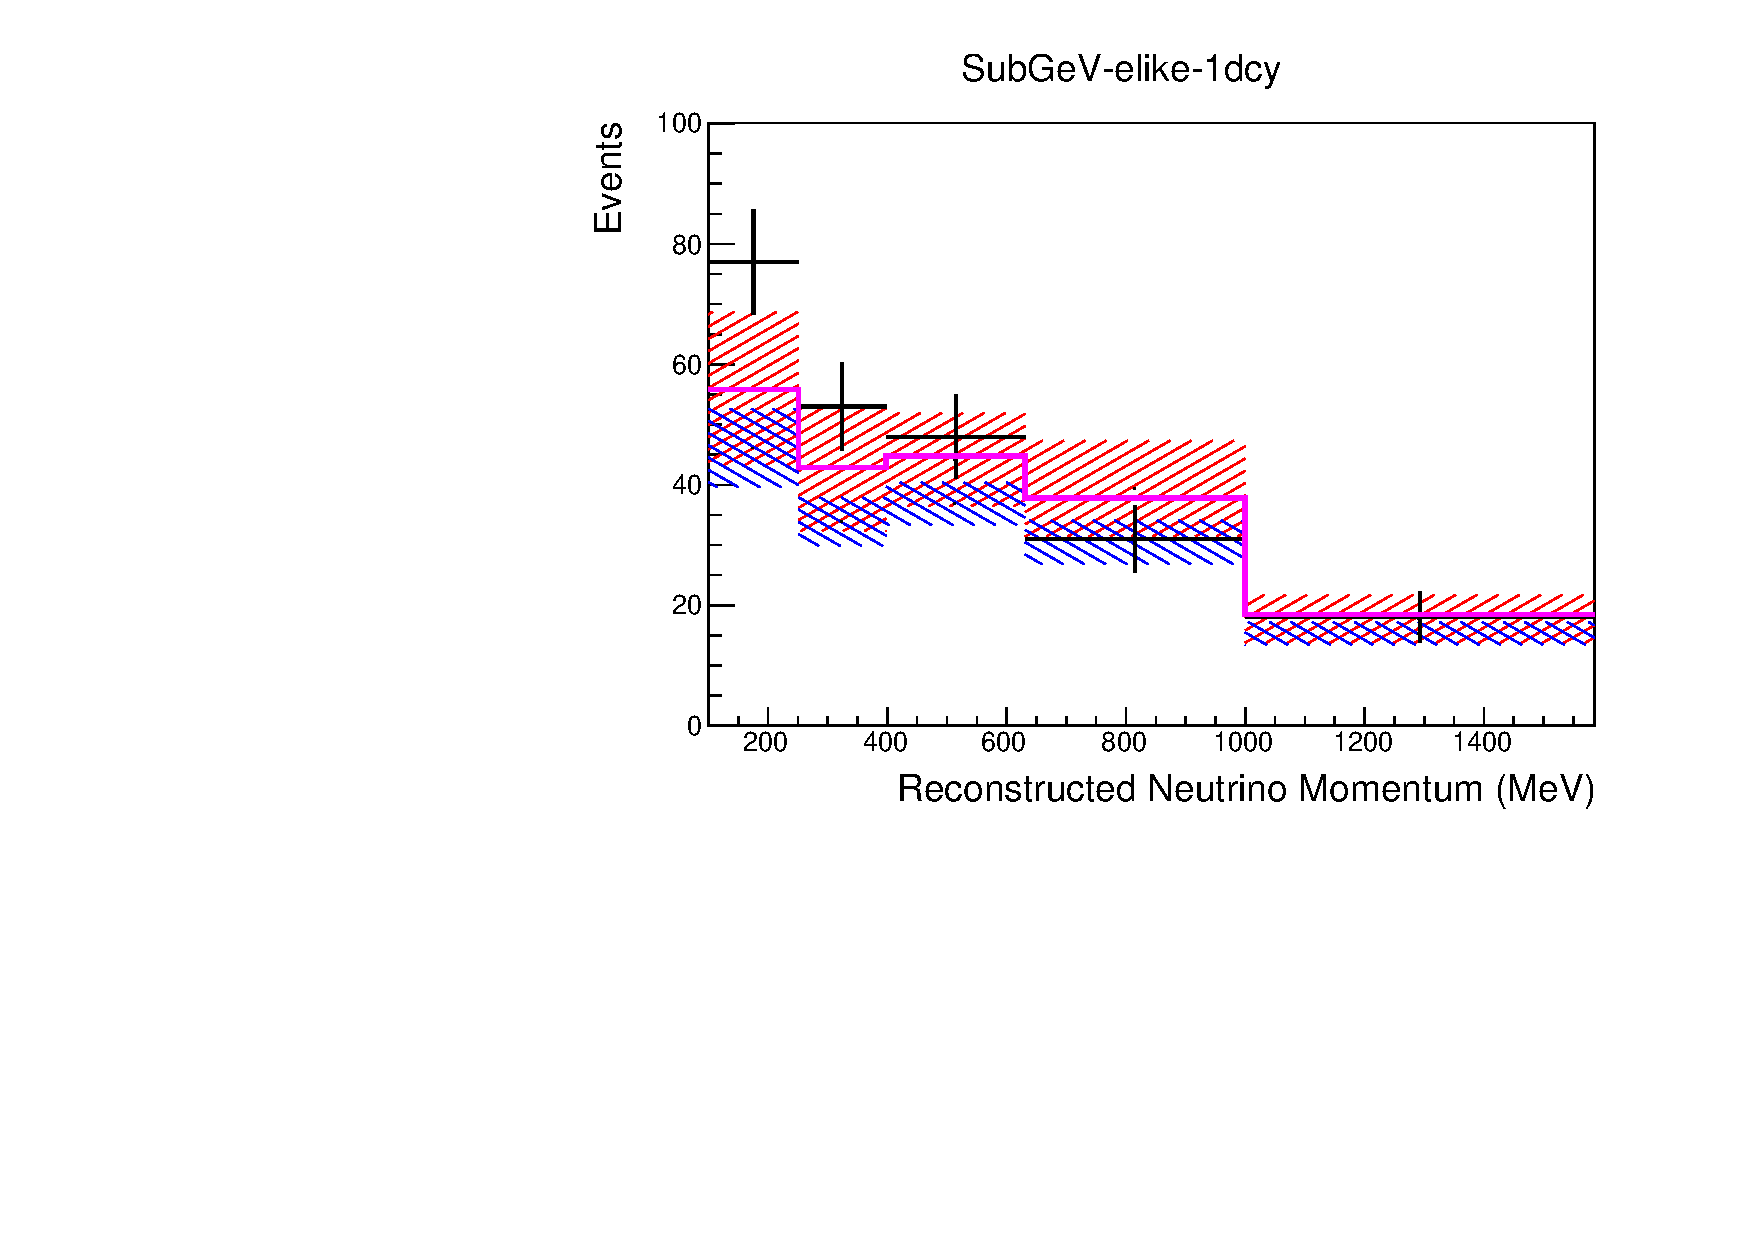
\includegraphics[width=\textwidth, trim={0mm 0mm 0mm 0mm}, clip,page=1]{Figures/Selections/Predictive_SubGeV-elike-1dcy.pdf}
  \end{subfigure}
  \begin{subfigure}[t]{0.49\textwidth}
    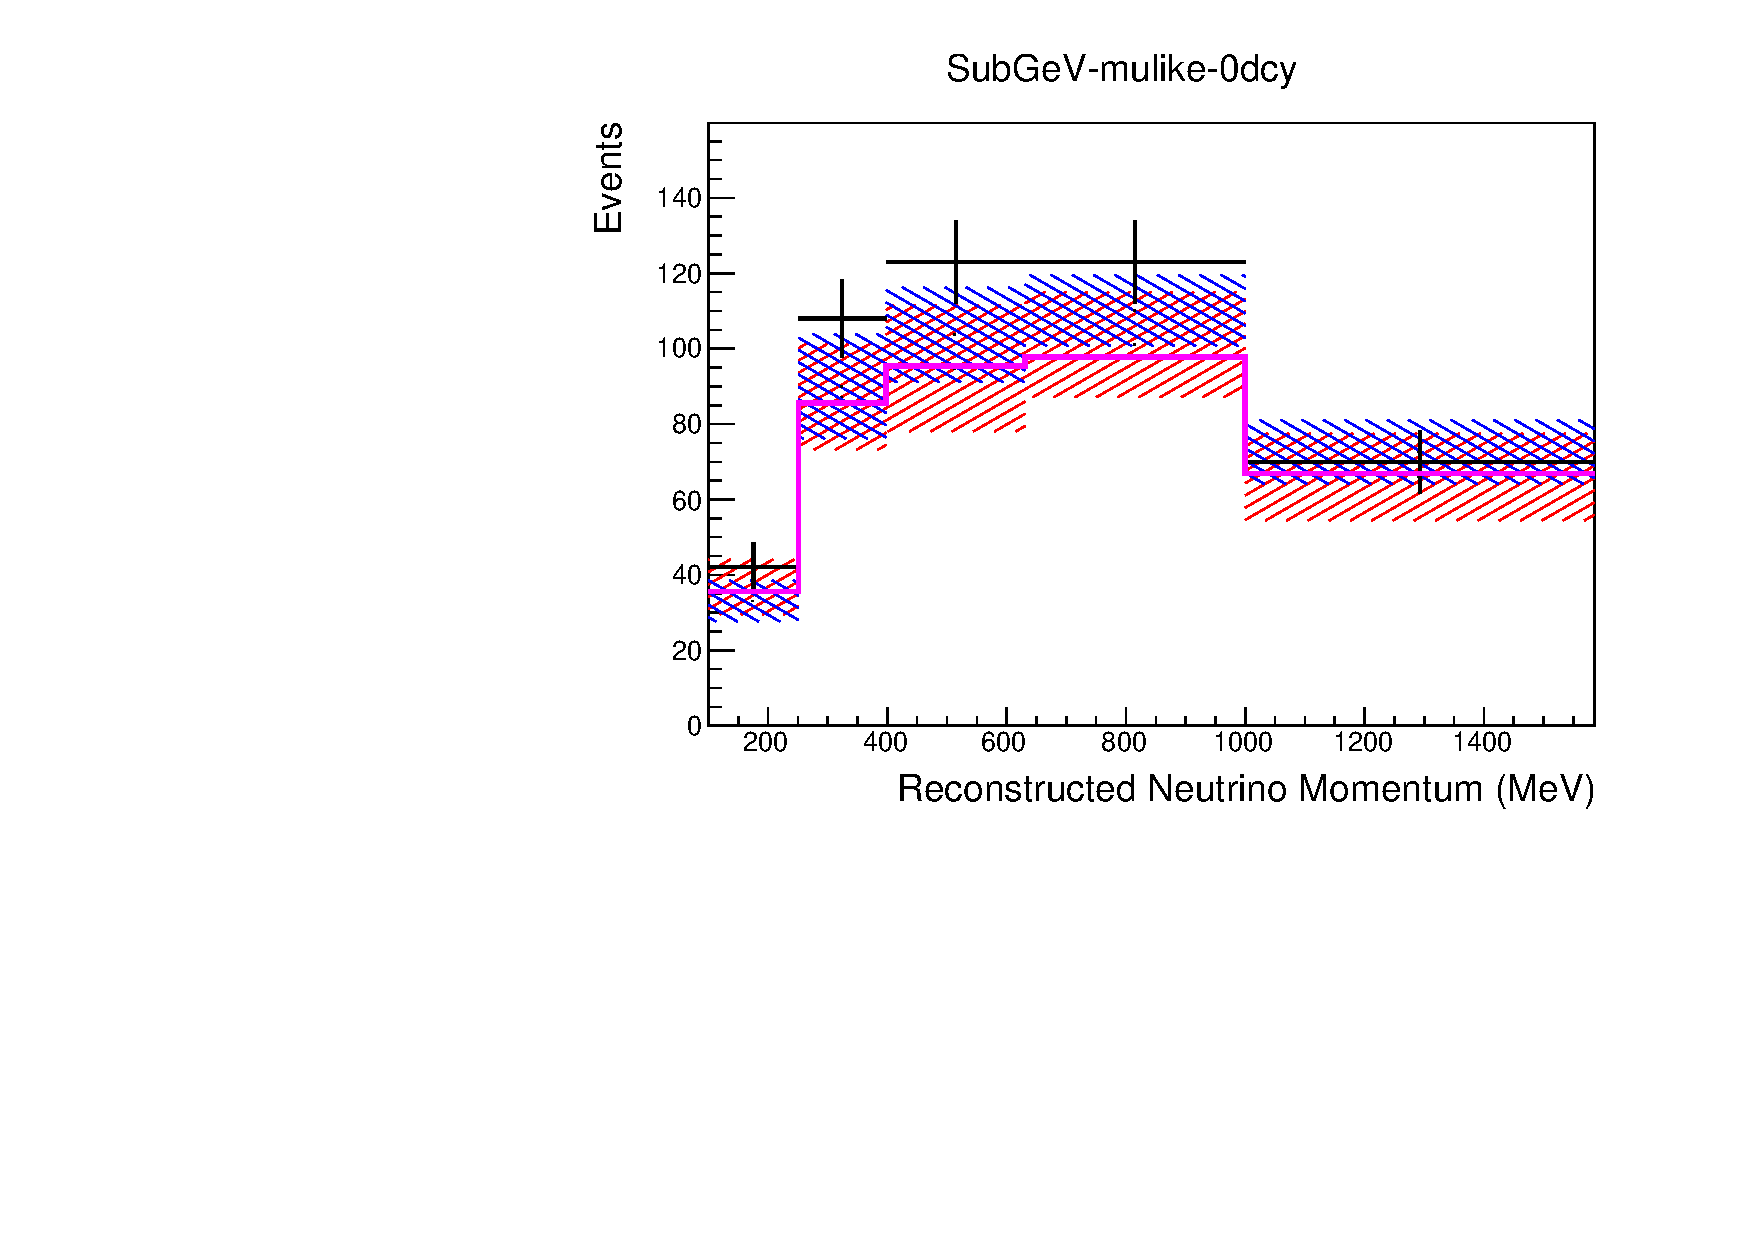
\includegraphics[width=\textwidth, trim={0mm 0mm 0mm 0mm}, clip,page=1]{Figures/Selections/Predictive_SubGeV-mulike-0dcy.pdf}
  \end{subfigure}%
  \begin{subfigure}[t]{0.49\textwidth}
    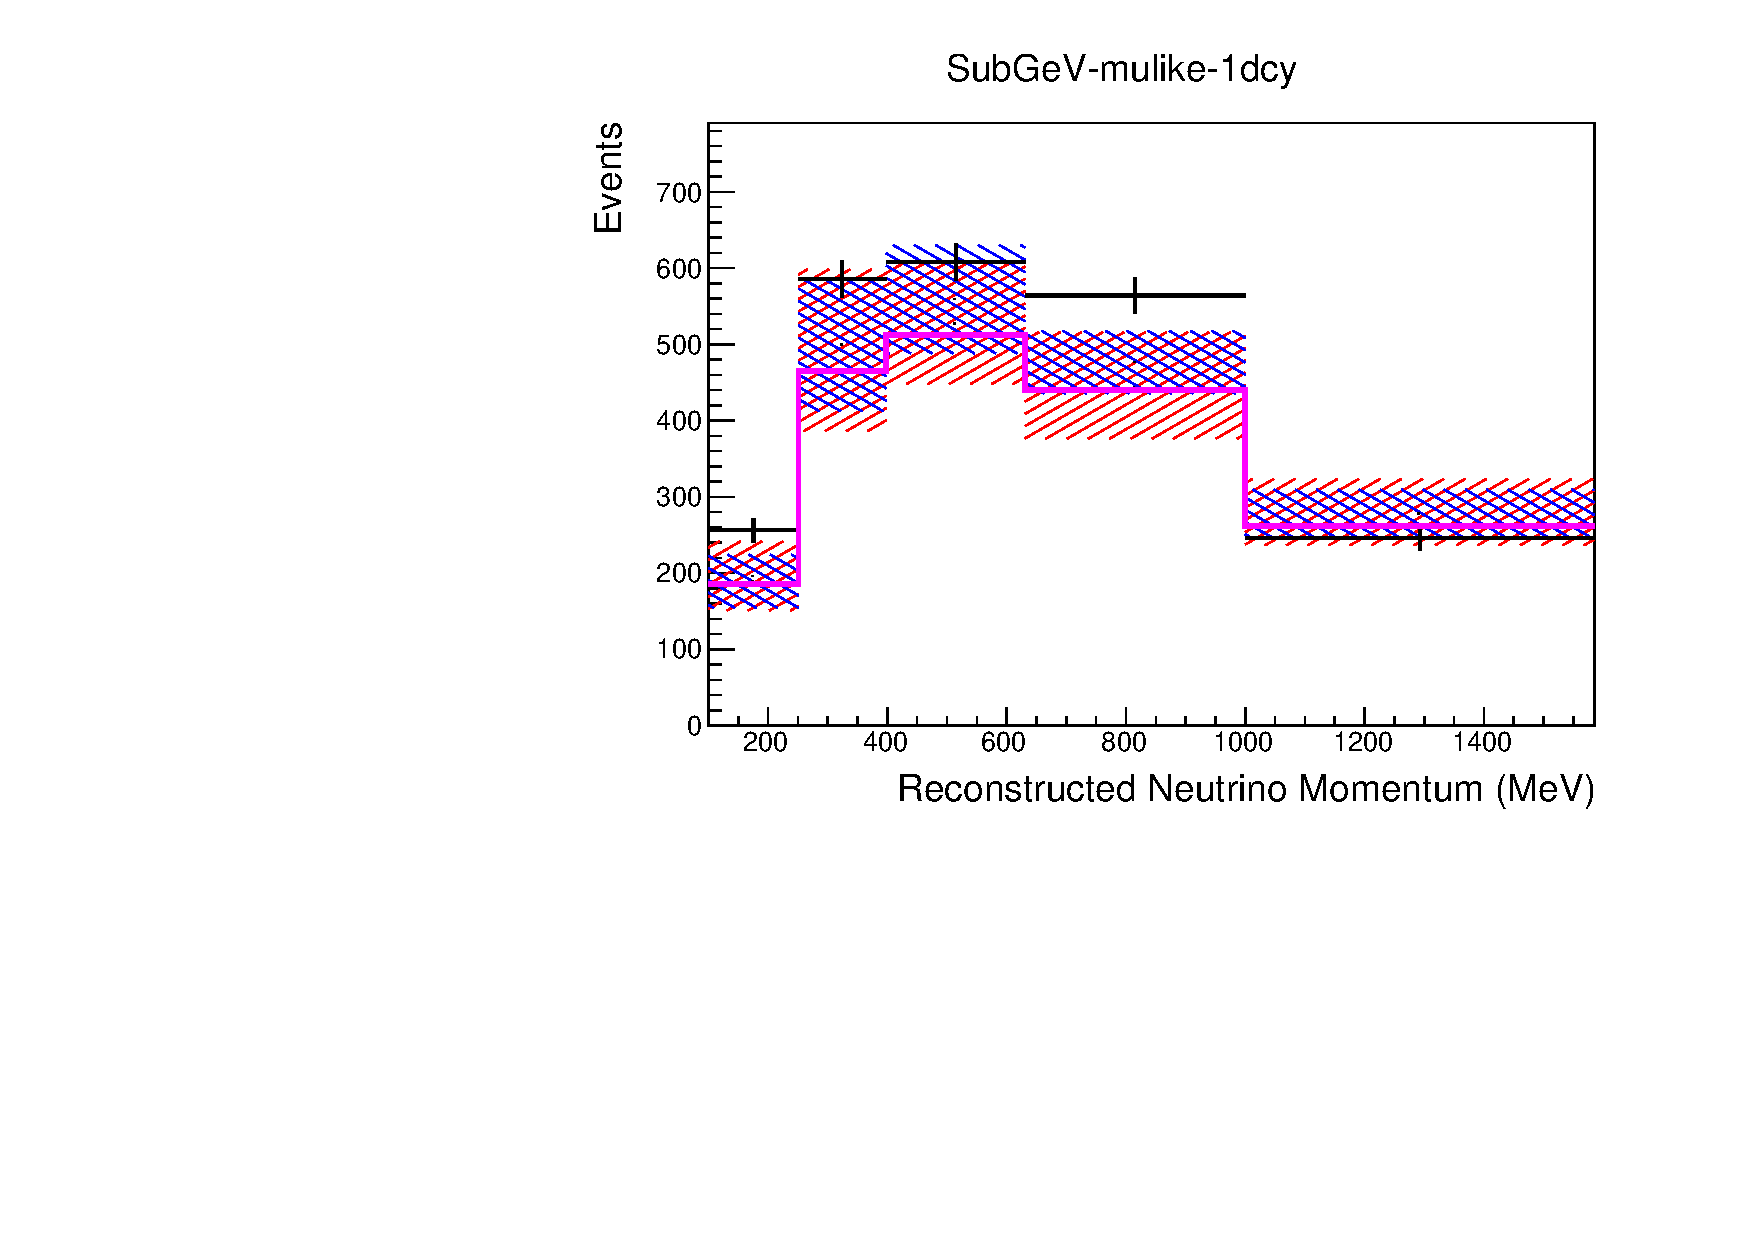
\includegraphics[width=\textwidth, trim={0mm 0mm 0mm 0mm}, clip,page=1]{Figures/Selections/Predictive_SubGeV-mulike-1dcy.pdf}
  \end{subfigure}
  \begin{subfigure}[t]{0.49\textwidth}
    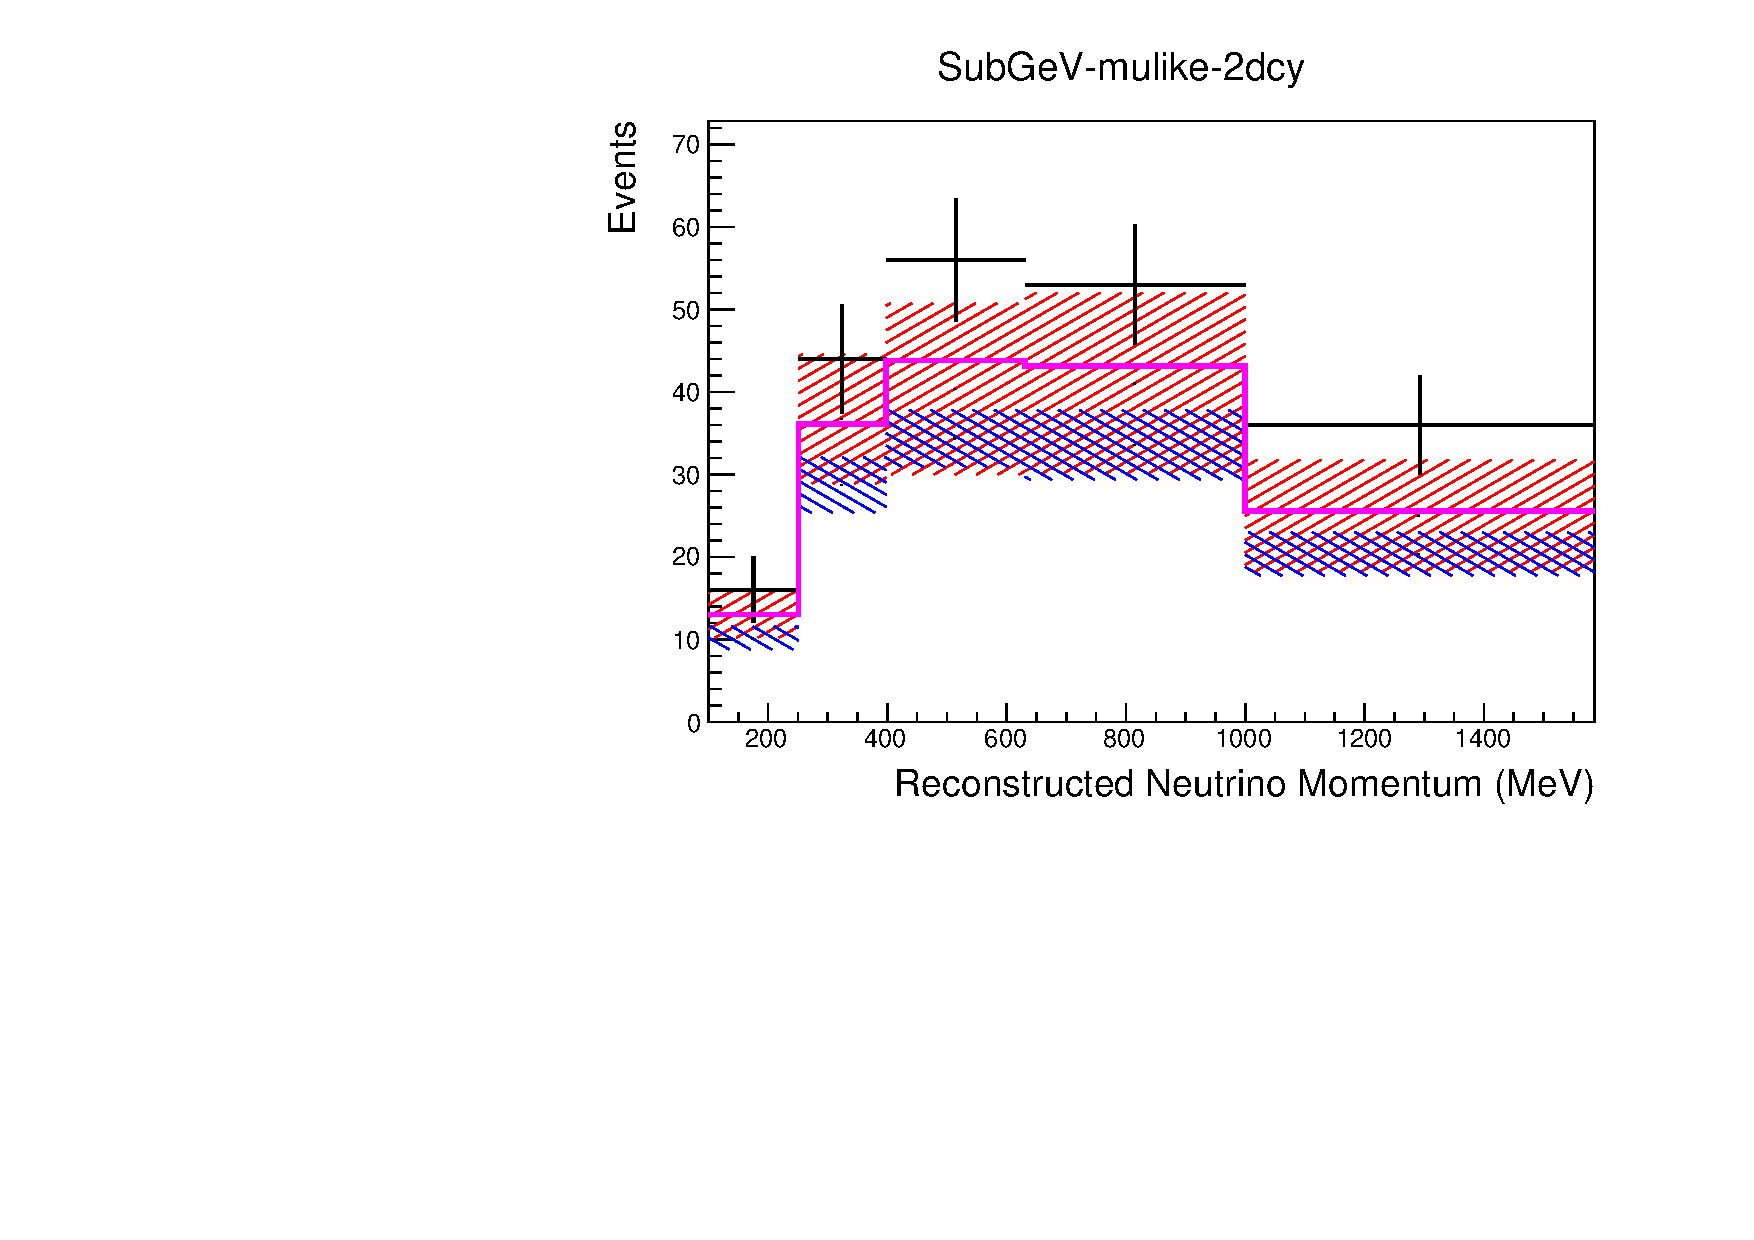
\includegraphics[width=\textwidth, trim={0mm 0mm 0mm 0mm}, clip,page=1]{Figures/Selections/Predictive_SubGeV-mulike-2dcy.pdf}
  \end{subfigure}
  \caption{Down-going atmospheric subGeV single-ring samples comparing the mean and error of the pre-fit and post-fit Monte Carlo predictions in red and blue, respectively. The magenta histogram illustrates the Monte Carlo prediction using the generated dial values. The black points illustrate the down-going data with statistical errors given. The mean and errors of the Monte Carlo predictions are calculated by the techniques documented in \autoref{sec:MarkovChainMonteCarlo_Predictives}. The cross-section and atmospheric flux parameters are either thrown from their pre-fit uncertainties (denoted pre-fit band), or the cross section dial values are randomly sampled from a MCMC chain whilst the atmospheric flux parameters are thrown from their pre-fit distributions (denoted post-fit band).}
  \label{fig:SelsAndSysts_DownGoingPredictives}
\end{figure}

\subsection{Near Detector}
\label{sec:SelsAndSysts_Systs_ND}

The systematics applied due to uncertainties arising from the response of the near detector is contained within \quickmath{574} normalisation parameters binned in momentum and angle, \quickmath{P_{\mu}} ad \quickmath{\cos(\theta_{\mu})}, of the final-state muon. These are applied via a covariance matrix with each parameter being assigned a Gaussian prior from that covariance matrix. These normalisation parameters are built from underlying systematics, e.g. pion secondary interaction systematics, which are randomly thrown and the variation in each \quickmath{P_{\mu} \times \cos(\theta_{\mu})} bin is determined. This is performed \quickmath{2000} times and a covariance matrix response is created. This allows significant correlations between FGD1 and FGD2 samples, as well as adjacent bins. Statistical uncertainties are accounted for by including fluctuations of each event's weight from a Poisson distribution.

Similar to the cross-section systematcs, MaCh3 and BANFF are used to constrain the uncertainty of these systematics through independent validations. Each fitter generates a post-fit covariance matrix which is compared and passed to the far-detector oscillation analysis working group. However, as the analysis presented within this thesis uses the MaCh3 framework, a joint oscillation analysis fit of all three sets of samples is performed. From the T2K-only perspective, this joint analysis including atmospheric samples allows additional constraints on the systematic uncertainties where correlations have been invoked. 

\subsection{Far Detector}
\label{sec:SelsAndSysts_Systs_FD}

Two configurations of the far detector systematic model implementation have been considered. Firstly, the far detector systematic uncertainties for beam and atmospheric samples are taken from their respective analysis inputs, denoted ``official inputs'' analysis. Consequently, no correlations are assumed between the beam and atmospheric samples. The generation of the beam- and atmospheric-specific inputs are documented in \autoref{sec:SelsAndSysts_Systs_FDBeam} and \autoref{sec:SelsAndSysts_Systs_FDAtm} for the beam and atmospheric samples, respectively. Secondly, a correlated detector model has been considered. Here, the distribution of parameters used for applying event cuts (e.g. electron-muon separation) is modified within the fit, following a similar methodology to the beam far detector systematics model implementation. However, it has been designed to ensure that the atmospheric data is not double-counted, which would be the case for the official-inputs analysis. This alternative implementation is detailed in \autoref{sec:SelsAndSysts_Systs_Correlated}.

\subsubsection{Beam Samples}
\label{sec:SelsAndSysts_Systs_FDBeam}

There are \quickmath{45} systematics which describes the response of the far detector, specifically for beam sample neutrino events. \quickmath{44} of these parameters are normalisation parameters and are split by the interaction mode, true neutrino flavour, reconstructed neutrino energy, and sample which they affect. The final parameter is the energy scale uncertainty. It is applied as a multiplicative factor to the reconstructed neutrino energy. The value of the systematic is taken from Monte Carlo to data differences illustrated in \cite{sk_2017}. The normalisation parameters are assigned a Gaussian error centralised at \quickmath{1.0} and a width taken from the covariance matrix. A detailed breakdown of the following procedure is found in \cite{t2k_tn_318}. To build the covariance matrix,  a fit is performed on atmospheric data which has been selected using beam sample selection cuts. The variable which defines each cut, \quickmath{L} (e.g. the electron-muon PID parameter) is assigned a smear, \quickmath{\alpha}, and shift, \quickmath{\beta} parameter such that,

\begin{equation}
  \label{eqn:SelsAndSysts_Systs_ShiftSmear}
  L^{i}_{j} \rightarrow \bar{L}^{i}_{j} = \alpha^{i}_{j} L + \beta^{i}_{j}
\end{equation}

Where \quickmath{L^{i}_{j}} (\quickmath{\bar{L}^{i}_{j}}) correspond to nominal(varied) PID cut parameters given in \autoref{tab:SelsAndSysts_Systs_CutVariables}. The shift and smear parameters are binned by final-state topology, \quickmath{j}, where the binning is given in \autoref{tab:SelsAndSysts_Systs_Topologies}. This approach is used to allow the cut parameter distributions to be modified within the fit which allows better data to Monte Carlo agreement.

\begin{table}[ht!]
    \centering
    \begin{tabular}{c|l}
      \hline
      Cut Variable & Parameter Name \\
      \hline
      \quickmath{0} & \fq \quickmath{e/\mu} PID \\
      \quickmath{1} & \fq \quickmath{e/\pi^{0}} PID \\
      \quickmath{2} & \fq \quickmath{\mu/\pi} PID \\
      \quickmath{3} & \fq Ring-Counting Parameter \\
      \hline
      \hline
    \end{tabular}
    \caption{List of cut variables that are included within the shift/smear fit documented in \cite{t2k_tn_318}.}      
    \label{tab:SelsAndSysts_Systs_CutVariables}
\end{table}

\begin{table}[ht!]
  \centering
  \begin{tabular}{c|l}
    \hline
    Category & Description \\
    \hline
    \quickmath{1e} & Only one electron above Cherenkov threshold in the final state \\
    \quickmath{1\mu} & Only one muon above Cherenkov threshold in the final state \\
    \quickmath{1e\text{+other}} & One electron and one or more other charged particles above \\
    & \hspace{0.2cm}Cerenkov threshold in the final state \\
    \quickmath{1\mu\text{+other}} & One muon and one or more other charged particles above \\
    & \hspace{0.2cm}Cerenkov threshold in the final state \\
    \quickmath{1\pi^0} & Only one $\pi^0$ in the final state\\
    \quickmath{1\pi^\pm} or \quickmath{1\text{p}} & Only one hadron (typically charged pion or proton) in the final state\\
    Other & Any other final state\\
    \hline
  \end{tabular}
  \caption{Reconstructed event topology categories on which the SK detector systematics \cite{t2k_tn_318} are based.}
  \label{tab:SelsAndSysts_Systs_Topologies}
\end{table}

Beyond the uncertainty on the PID cut criteria, the mis-modeling of \quickmath{\pi^{0}} events is also considered. If one of the two rings from a \quickmath{\pi^{0}} event is missed, this will be reconstructed as a CC\quickmath{\nu_{e}} event. This is one of the largest systematics hindering the electron neutrino appearance analyses. Consequently, a systematic has been introduced to constrain the mis-modeling of \quickmath{\pi^{0}} events in SK. To evaluate this systematic uncertainty, a set of “hybrid-\quickmath{\pi^{0}} samples is constructed. These events are built by overlaying one electron-like ring from the SK atmospheric neutrino samples or decay electron ring from a stopping cosmic ray muon with one simulated photon ring. Both rings are chosen so that momenta and opening angle follow the decay kinematics of NC \quickmath{\pi^0} events from the T2K-MC. Hybrid-\quickmath{\pi^{0}} Monte Carlo samples with both rings from the SK Monte Carlo are produced to compare with the hybrid-\quickmath{\pi^{0}} data samples and the difference in the fraction of events that pass the \quickmath{\nu_{e}} selection criteria is used to assign the systematic error. In order to investigate any data to Monte Carlo differences that may originate from either the higher energy ring or lower energy ring, two samples are built; a sample in which the electron constitutes the higher energy ring from the \quickmath{\pi^{0}} decay called the primary sample and another one in which it constitutes the lower energy ring called the secondary sample. The standard T2K \quickmath{\nu_{e}} fiTQun event selection criteria are used to select events.

Final contributions to the covariance matrix are determined by supplementary uncertainties attained by comparing stopping muon data to Monte Carlo prediction, as first introduced in \autoref{sec:Simulation_Reconstruction}. The efficiency of tagging decay electrons is estimated by the stopping muon data/Monte Carlo differences by comparing the number of one decay electron events to the number of events with one or fewer decay electrons. The rate at which fake decay electrons are reconstructed by \fq is estimated in a similar way with the only difference being the ratio compares the number of two decay electron events to the number of events with one or two reconstructed decay electrons. The two sources of systematics are added in quadrature weighted by the number of events with one true decay electron yielding a \quickmath{0.2\%} systematic uncertainty. The muon misidentification rate is estimated by comparing the number of electron-like events which have one decay electron to the total number of events with one decay electron. This systematic is estimated as a \quickmath{30\%} effect in the rate of muon misidentification. A fiducial volume systematic of \quickmath{\pm 2.5\text{cm}} which corresponds to a \quickmath{0.5\%} shift in the normalisation of events. Additional normalisation uncertainties based on neutrino flavour and interaction mode are also defined in \cite{t2k_tn_326, t2k_tn_186, t2k_tn_107}.

This covariance matrix is then added in quadrature with two other covariance matrices. These are matrices that describe the uncertainties due to secondary interactions which modify the final state kinematics and the photo-nucleon interactions. These are generated by studying the effect of each sample's event rates when considering variations of the underlying parameters.

\subsubsection{Atmospheric Samples}
\label{sec:SelsAndSysts_Systs_FDAtm}

The systematic parameters which control the detector systematics are split into two sub-groups. Those which are related to particle identification and ring counting systematics and those which are related to calibration measurements. 

The particle identification systematics consist of five parameters. The ring separation systematic enforces an anti-correlated response between the single-ring and multi-ring samples. This is implemented as a fractional increase/decrease in the overall normalisation of each sample, depending on the distance to the nearest wall from an event's vertex. The coefficients of the normalisation are estimated prior to the fit and depend on the atmospheric sample. The single-ring and multi-ring PID systematics encode the detector's ability to separate electron-like and muon-like events and are implemented in an identical way to the ring separation systematic.

The multi-ring electron-like separation systematics encode the ability of the detector to separate neutrino from anti-neutrino events. As an important systematic in the mass hierarchy determination, this systematic controls the relative normalisation's of the \quickmath{\nu_e} and \quickmath{\bar{\nu}_e} enriched samples. A two-stage approach is implemented in the event selection and a systematic is implemented for both stages. The first stage in the event selection is to confirm that the most energetic ring, which is required to be electron-like, is from the neutrino interaction rather than a pion decay from any hadronic system present in the event. The second stage of separation uses a likelihood-based cut to separate \quickmath{\nu_e/\bar{\nu}_e} events. This takes the typical properties of \quickmath{\nu_e} scattering events into account; e.g. less forward-going, with larger energy fractions in the hadronic system. These parameters are implemented via normalisation parameters which vary the event rate of each multi-ring sample, whilst ensuring the total event rate is conserved.

There are 22 systematics related to calibration measurements, including effects from backgrounds, reduction, and showering effects. They are documented in \cite{Jiang2019-iw} are briefly summarised in \autoref{SelsAndSysts_Systs_ATMPDCalibSysts}. They are applied via normalisation parameters, with the separation systematics requiring the conservation of event rate across all samples.

\begin{table}[ht!]
  \centering
  \caption{Sources of systematic errors specified within the grouped into the ``calibration'' systematics model.}
  \label{SelsAndSysts_Systs_ATMPDCalibSysts}
		
  \begin{tabular}{ll} 
    
    \hline Index & Description \\ 
    \hline
    0 & Partially contained reduction  \\
    1 & Fully contained reduction \\
    2 & Separation of fully contained and partially contained events \\
    3 & Separation of stopping and through-going\\
      & \hspace{0.4cm} partially contained events in top of detector \\
    4 & Separation of stopping and through-going\\
      & \hspace{0.4cm} partially contained events in barrel of detector \\
    5 & Separation of stopping and through-going\\
      & \hspace{0.4cm} partially contained events in bottom of detector \\
    6 & Background due to cosmic rays \\
    7 & Background due to flasher events \\
    8 & Vertex systematic moving events into and out of fiducial volume \\
    9 & Upward going muon event reduction \\
    10 & Separation of stopping and through-going in upward going muon events \\
    11 & Energy systematic in upward going muon events \\
    12 & Reconstruction of the path length of upward going muon events \\
    13 & Separation of showering and non-showering upward going muon events \\
    14 & Background of stopping upward going muon events \\
    15 & Background of non-showering through-going upward going muon events \\
    16 & Background of showering through-going upward going muon events \\
    17 & Efficiency of tagging two rings from $\pi^0$ decay \\
    18 & Efficiency of decay electron tagging \\
    19 & Background from downgoing cosmic muons \\
    20 & Asymmetry of energy deposition in tank \\
    21 & Energy scale deposition \\
    \hline
  \end{tabular}
\end{table}

\subsubsection{Correlated Detector Model}
\label{sec:SelsAndSysts_Systs_Correlated}

A complete uncertainty model of the SK detector would be able to determine the systematic shift on the sample spectra for a variation of the underlying parameters, e.g. PMT angular acceptance. However, this is computationally intensive, requiring Monte Carlo predictions to be made for each plausible variation. Consequently, an effective parameter model has been utilised for a correlated detector model. This follows from the T2K-only model implementation documented in \autoref{sec:SelsAndSysts_Systs_FDBeam}. The T2K-only implementation can not be used for atmospheric sample systematics because it is built upon a fit to atmospheric data. Consequently, an implementation where the cut distributions (given in \autoref{tab:SelsAndSysts_Systs_CutVariables}) from both beam and atmospheric samples are fit, whilst simultaneously fitting for oscillation parameters. The fit to the cut variables performs a shape-only fit to ensure that no double-counting occurs.

The correlated detector model utilises the same smear and shift parameters documented in \autoref{sec:SelsAndSysts_Systs_FDBeam}, split by final state topology. This splitting is done because the detector will respond differently to events that have one or multiple rings. For example, the detector will be able to distinguish single-ring events better than two overlapping ring events, resulting in smaller systematic uncertainty for one-ring events compared to two-ring events. Furthermore, the shift and smear parameters are split by visible energy deposited within the tank has been included, with binning specified in \autoref{tab:SelsAndSysts_Systs_EVisBinning}. This is because atmospheric events are categorised by subGeV and multiGeV events based on visible energy, so this splitting is required when correlating the systematic model for beam and atmospheric events. Alongside the technical requirement, higher energy events will be better reconstructed due to fractionally less noise within the detector. Consequently, this analysis correlates the detector systematics between the far-detector beam and subGeV atmospheric samples due to their similar energies and interaction types. As a result of the inclusion of visible energy binning, \autoref{eqn:SelsAndSysts_Systs_ShiftSmear} becomes

\begin{equation}
  \label{eqn:SelsAndSysts_Systs_ShiftSmearWithEVis}
  L^{i}_{jk} \rightarrow \bar{L}^{i}_{jk} = \alpha^{i}_{jk} L + \beta^{i}_{jk},
\end{equation}

where \quickmath{k} is the visible energy bin. The multi-GeV, multi-ring, PC, and Up-\quickmath{\mu} samples will be subject to the ATMPD particle identification systematics implementation as described in \autoref{sec:SelsAndSysts_Systs_FDAtm} rather than using this correlated detector model. The calibration systematics also described in the aforementioned chapter still apply to all atmospheric samples.

\begin{table}[ht!]
    \centering
    \begin{tabular}{c|c}
      \hline
      Index & Range (MeV) \\
      \hline
      \quickmath{0} & \quickmath{30 \geq x > 300} \\
      \quickmath{1} & \quickmath{300 \geq x > 700} \\
      \quickmath{2} & \quickmath{700 \geq x > 1330} \\
      \quickmath{3} & \quickmath{1330 \geq x} \\
      \hline
      \hline
    \end{tabular}
    \caption{Reconstructed event topology categories on which the SK detector systematics are based}
    \label{tab:SelsAndSysts_Systs_EVisBinning}
\end{table}

The implementation of this systematic model takes the events reconstructed values of the cut parameters, modifies them by the particular shift and smear parameter for that event, and then re-applies event selection. This invokes event migration, which is a new feature incorporated into the MaCh3 framework which is only achievable due to the event-by-event reweighting scheme.

Particular care has to be taken when varying the ring counting parameter. This is because the number of rings is a finite value (one-ring, two-rings, etc.) which can not be continuously varied. Consequently a ring counting parameter, \quickmath{RC_{i}}, is calculated for the \quickmath{i^{th}} event, following the definition in \cite{Tobayama:2016dsi}. The likelihood from all considered one-ring (\quickmath{1R}) and two-ring (\quickmath{2R}) fits are compared to determine the preferred hypothesis. This is done by searching for the minimum log-likelihoods, \quickmath{\log(L_{1R})} and \quickmath{\log(L_{2R})}. The difference is computed as \quickmath{\Delta_{LLH} = \log(L_{1R}) - \log(L_{2R})}. The ring counting parameter is then defined as,

\begin{equation}
  \label{eqn:SelsAndSysts_Systs_RCParam}
  RC_{i} = \text{sgn} \left(\Delta_{LLH} - C_{Thres} \right) \times \sqrt{\lvert \Delta_{LLH} - C_{Thres} \rvert},
\end{equation}

where \quickmath{C_{Thres} = 150.0 - 0.6 \times P_{2R}}, and \quickmath{P_{2R}} is the momentum of the preferred two-ring hypothesis, and \quickmath{\text{sgn}(x) = x/\lvert x \rvert}. The coefficients used within the definition of \quickmath{C_{Thres}} are calculated based on Monte Carlo studies. This ring counting parameter corresponds to an intermediate likelihood value used within the \fq algorithm to decide the number of rings associated with a particular event. However, fake-ring merging algorithms are applied after this likelihood value is used to determine the number of rings associated with an event. Consequently, this ring counting parameter does not always exactly correspond to the number of reconstructed rings. This can be seen in \autoref{fig:SelsAndSysts_RCParameterDistribution}.

\begin{figure}[h]
  \begin{subfigure}[t]{0.49\textwidth}
    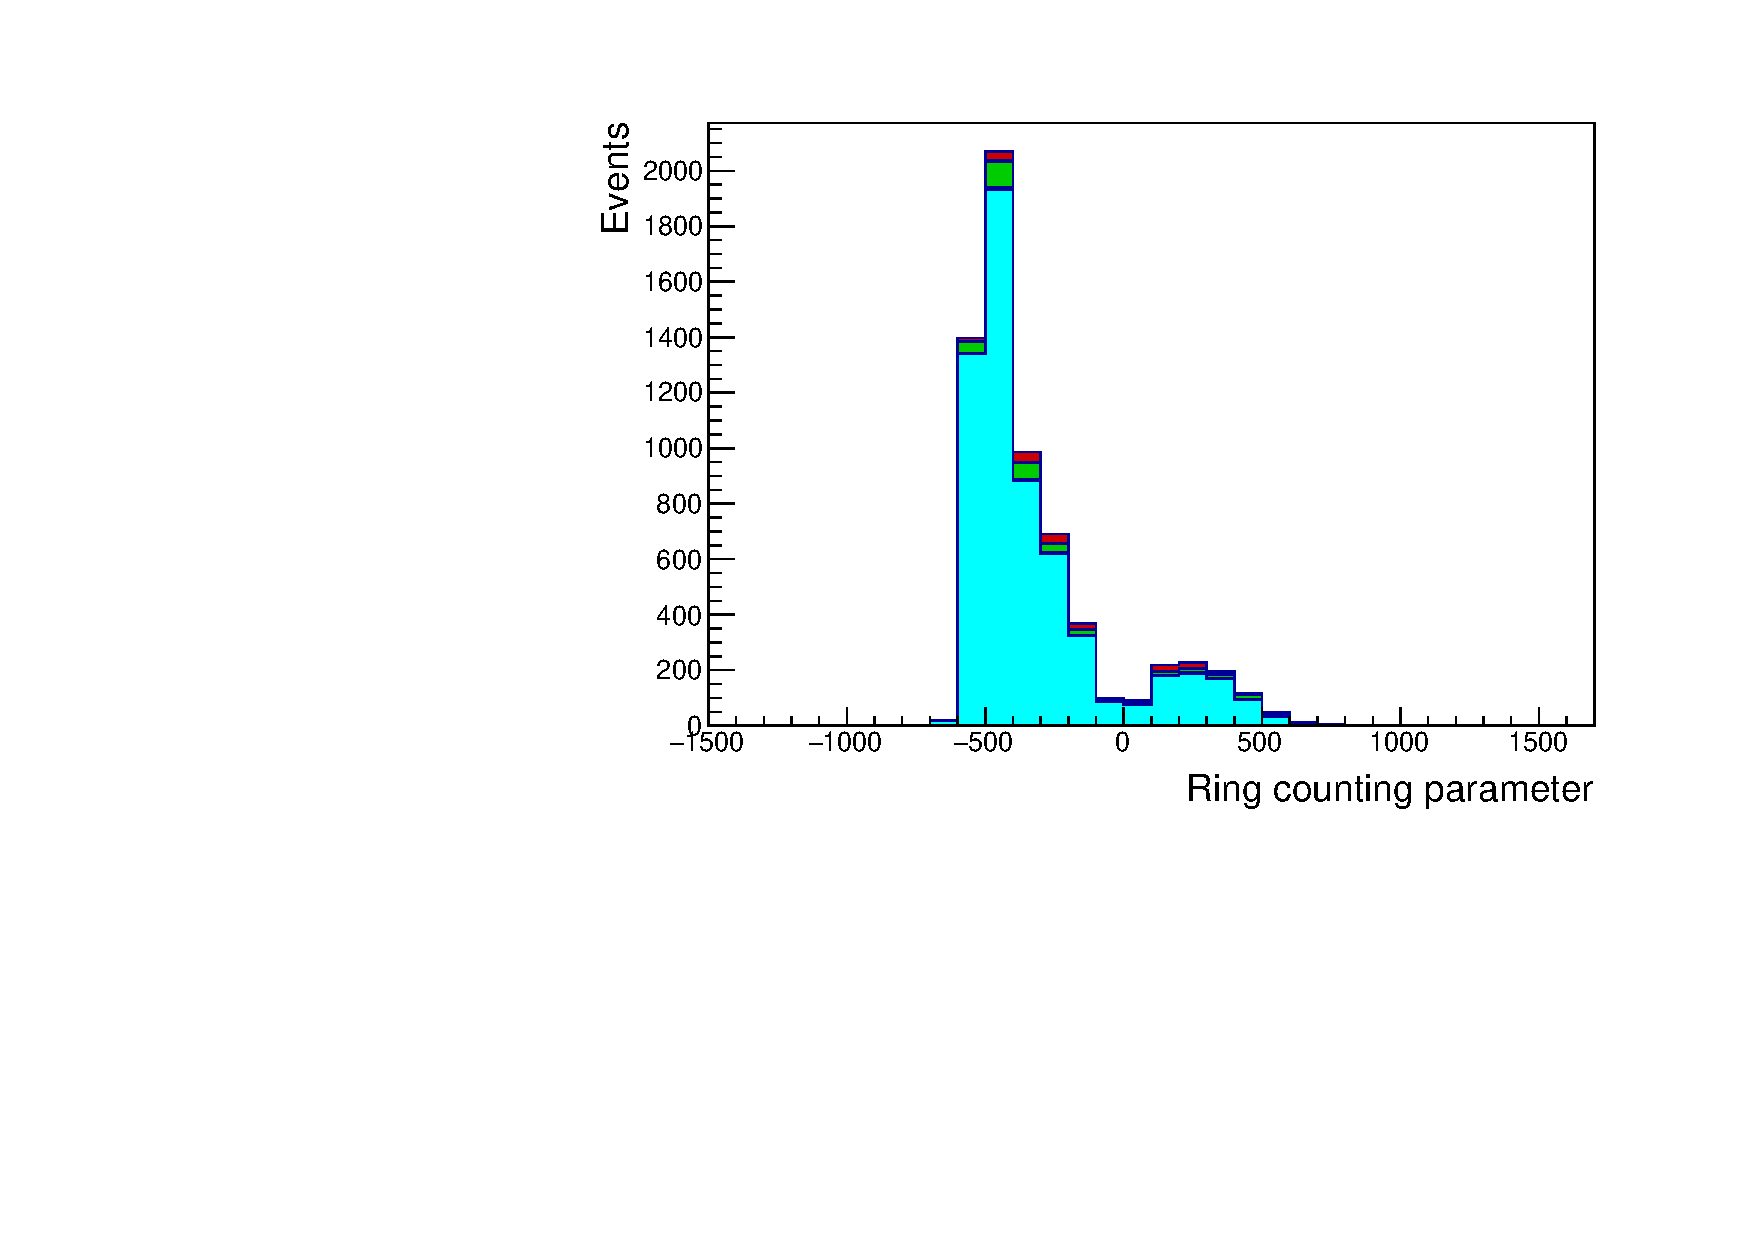
\includegraphics[width=\textwidth, trim={0mm 0mm 0mm 0mm}, clip,page=1]{Figures/Selections/RCParam_SGE0Dcy.pdf}
    \subcaption{SubGeV e-Like 0d.e.}
  \end{subfigure}%
  \begin{subfigure}[t]{0.49\textwidth}
    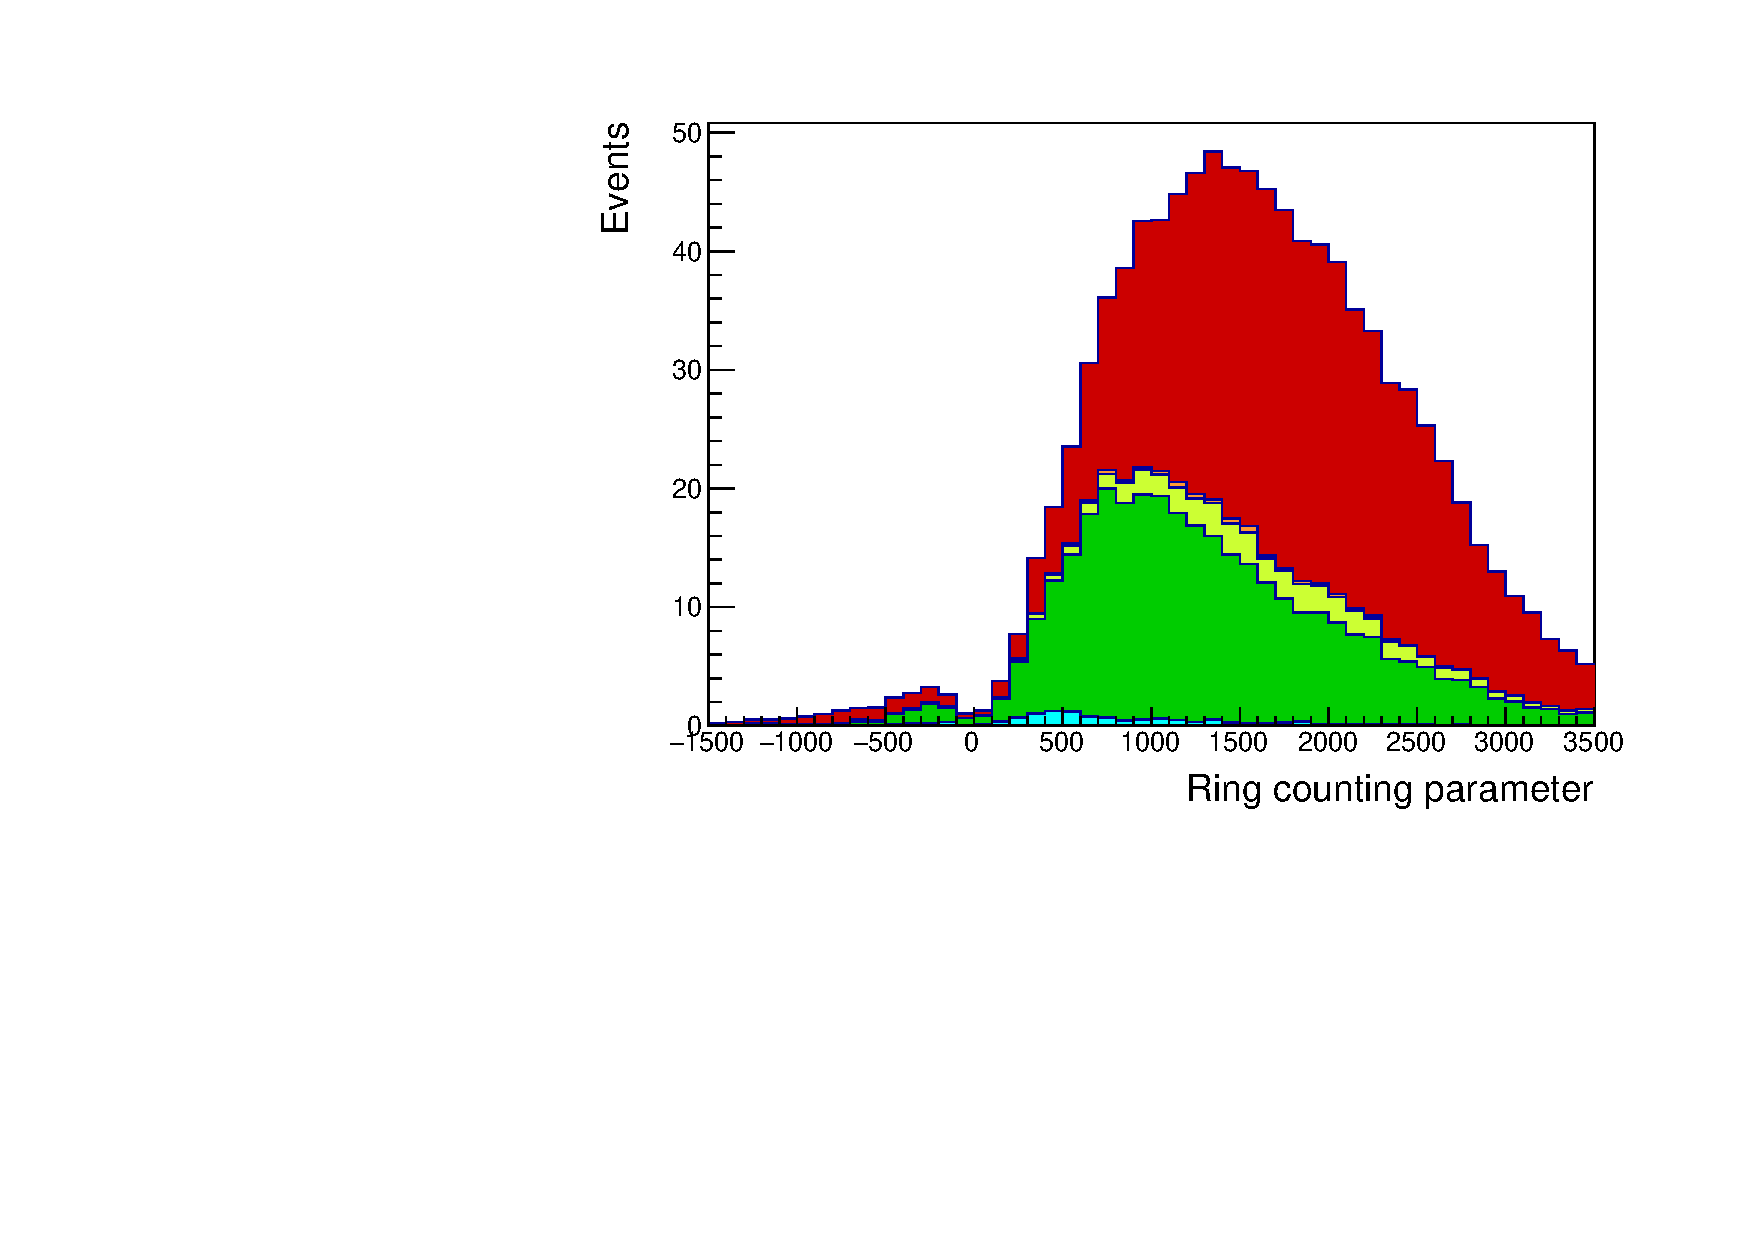
\includegraphics[width=\textwidth, trim={0mm 0mm 0mm 0mm}, clip,page=1]{Figures/Selections/RCParam_MRENue.pdf}
    \subcaption{MultiRing \quickmath{\nu_{e}}-Like}
  \end{subfigure}
  \begin{subfigure}[t]{0.49\textwidth}
    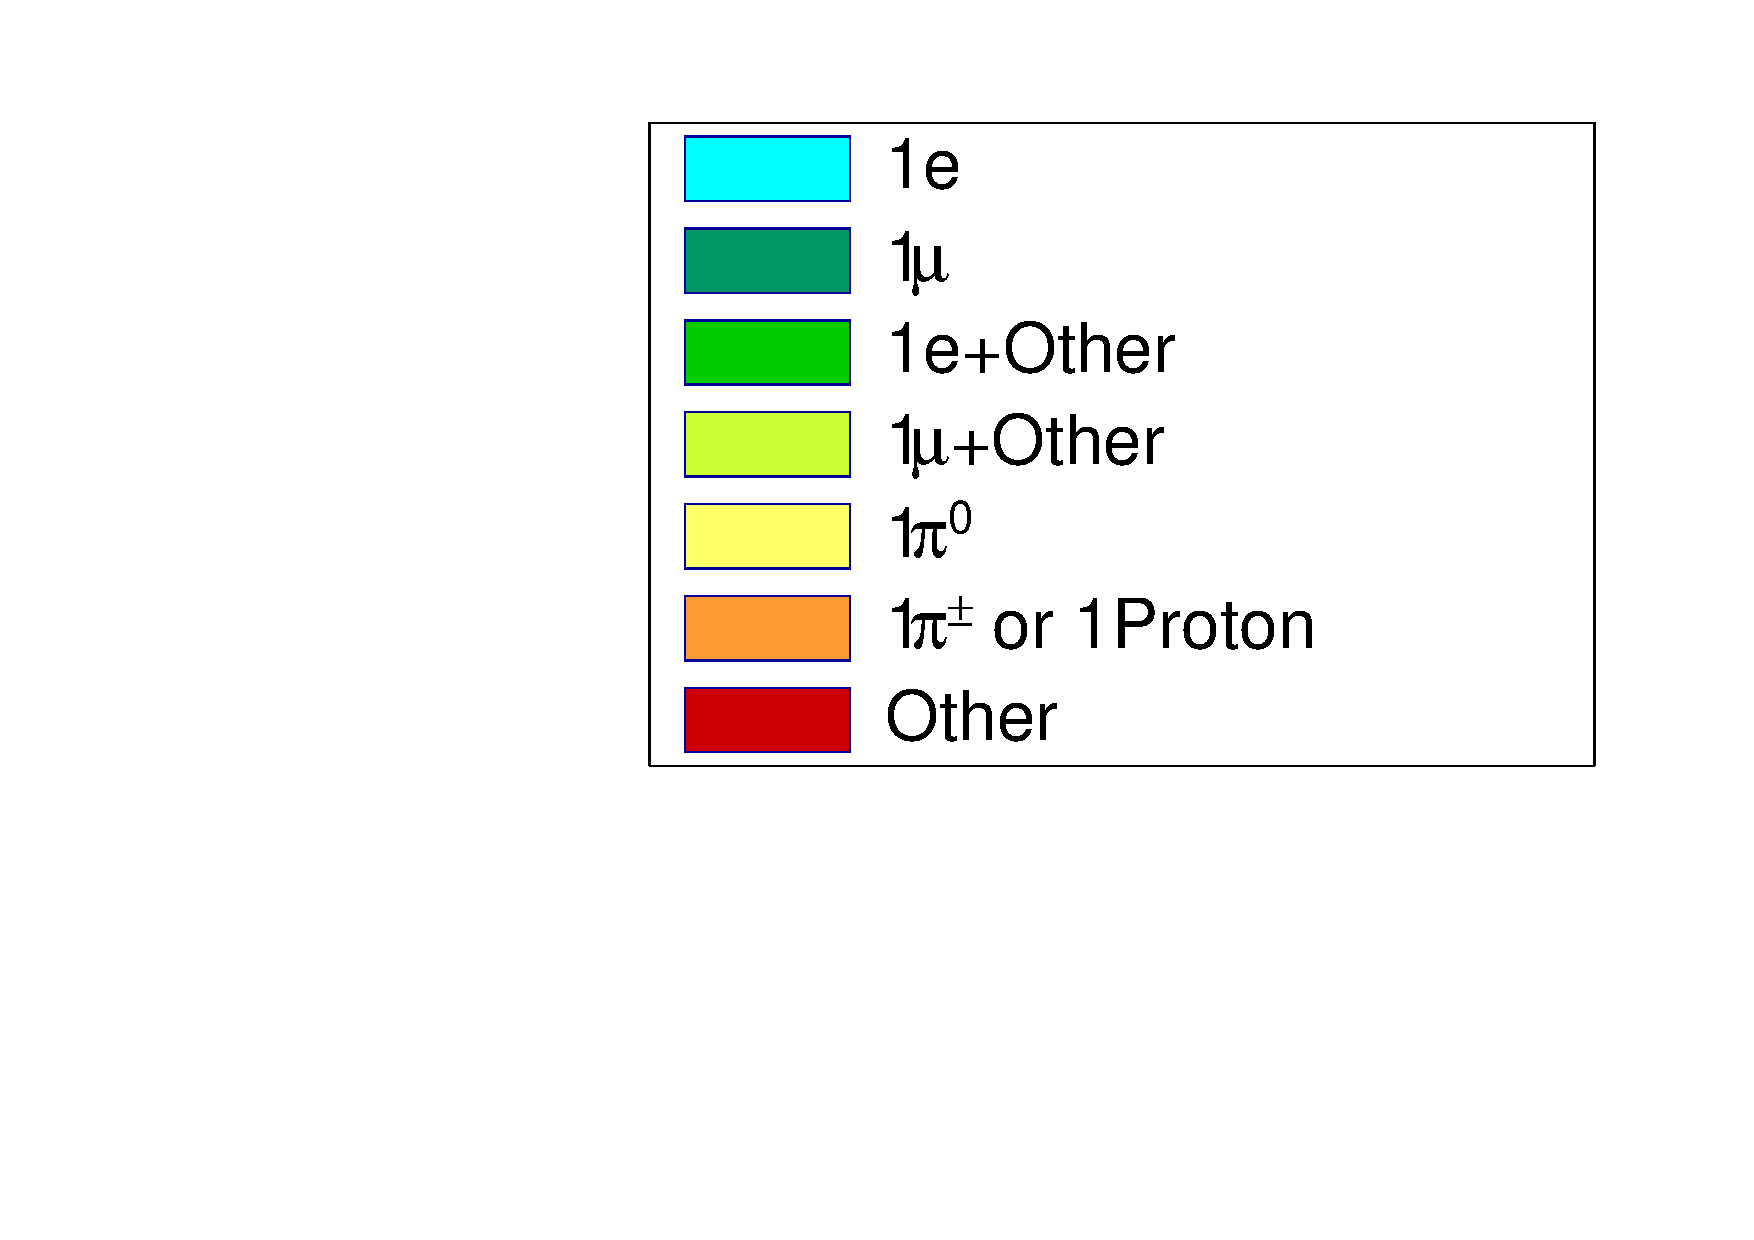
\includegraphics[width=\textwidth, trim={0mm 0mm 0mm 0mm}, clip,page=1]{Figures/Selections/RCParameterLegend.pdf}
  \end{subfigure}
  \caption{The ring counting parameter, as defined in \autoref{eqn:SelsAndSysts_Systs_RCParam}, for the subGeV electron-like zero decay electron and multi-ring \quickmath{\nu_{e}}-like samples.}
  \label{fig:SelsAndSysts_RCParameterDistribution}
\end{figure}

As the \fq algorithm does not provide a likelihood value after the fake-ring algorithms have been applied, the ring counting parameter distribution is connected to the final number of reconstructed rings through ``maps''. These are two-dimensional distributions linking the ring counting parameter and the final number of reconstructed rings. An example is illustrated in \autoref{fig:SelsAndSysts_RCMaps}. In principle, the \fq reconstruction algorithm should be re-run after the variation in the ring counting parameter. However, this is not computationally viable. Therefore the ``maps'' are used as a reweighting template.

The maps are split by final state topology and true neutrino flavour and all \fq-reconstructed Monte Carlo events are used to fill them. To ensure the conservation of event rate, the maps are normalised such that the total event rate across all number of reconstructed rings is equal to one. Prior to the fit, an event's nominal weight is calculated as \quickmath{W(N^{i}_{Rings},L^{i}_{jk})}, where \quickmath{N^{i}_{Rings}} is the reconstructed number of rings for the \quickmath{i^{th}} event and \quickmath{W(x,y)} is the bin content in the associated map for \quickmath{x} number of rings and ring counting parameter \quickmath{L}. Then during the fit, the value of \quickmath{R = W(N^{i}_{Rings},\bar{L}^{i}_{jk})/W(N^{i}_{Rings},L^{i}_{jk})} is calculated as the ring-counting weight for the \quickmath{i^{th}} event. This is the only cut variable that uses a reweighting scheme rather than event migration.

\begin{figure}[h]
  \begin{subfigure}[t]{0.49\textwidth}
    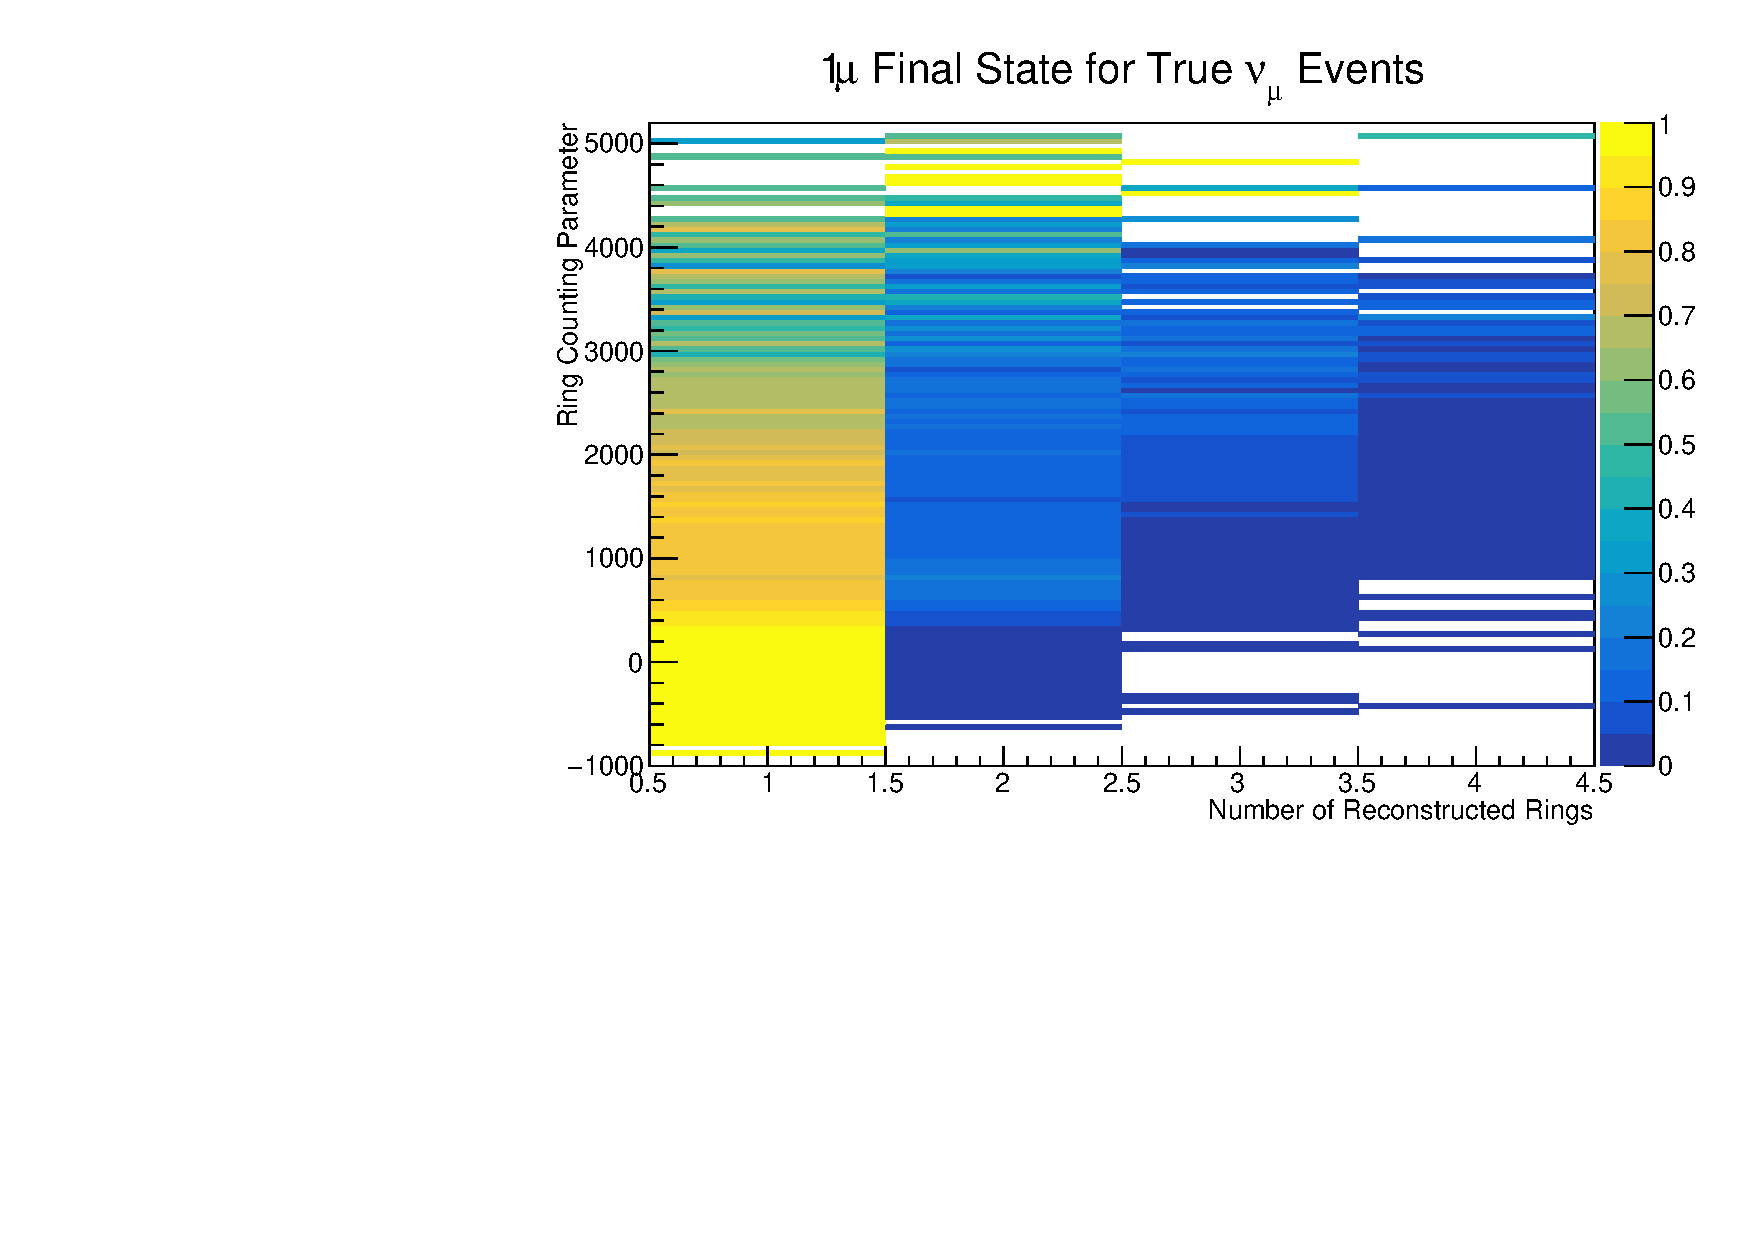
\includegraphics[width=\textwidth, trim={0mm 0mm 0mm 0mm}, clip,page=1]{Figures/Selections/NuFlavour_14_Top_1.pdf}
  \end{subfigure}%
  \begin{subfigure}[t]{0.49\textwidth}
    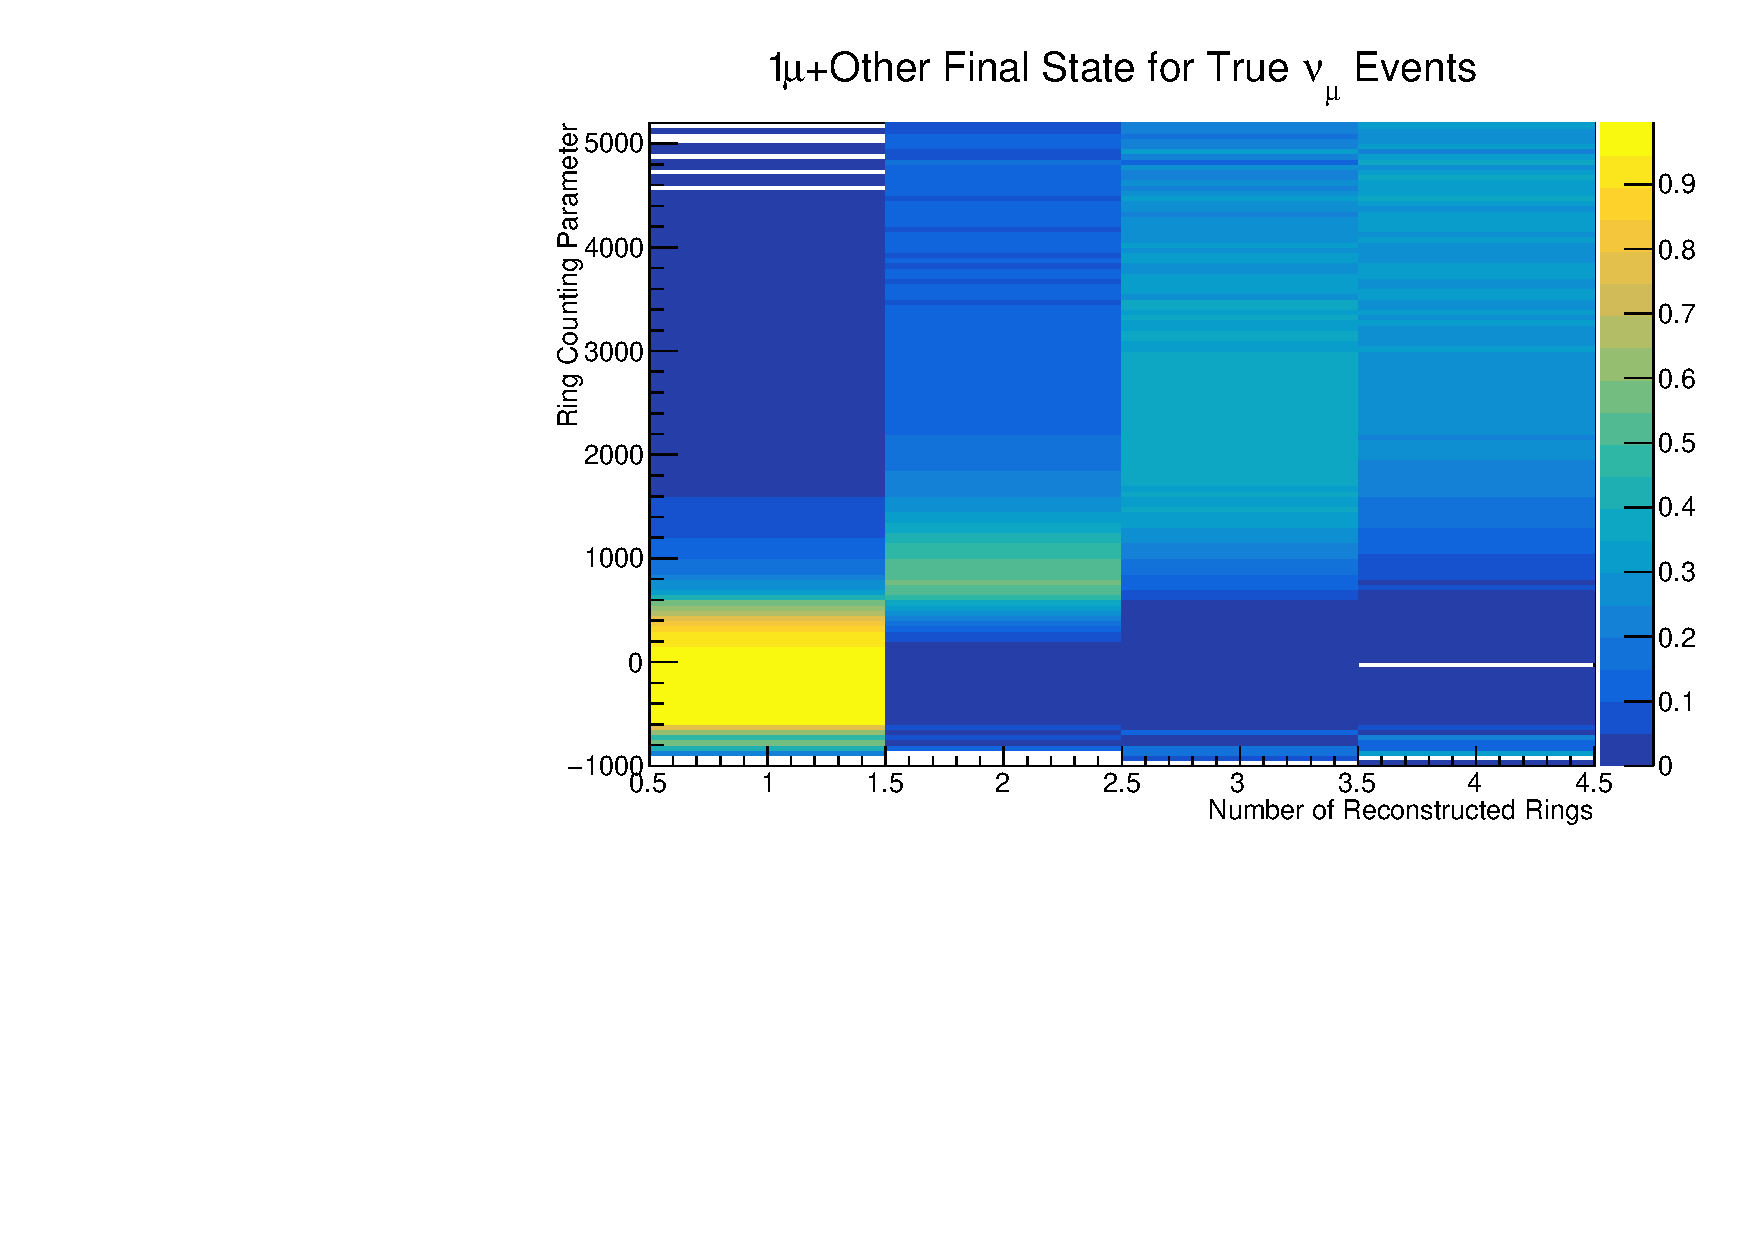
\includegraphics[width=\textwidth, trim={0mm 0mm 0mm 0mm}, clip,page=1]{Figures/Selections/NuFlavour_14_Top_3.pdf}
  \end{subfigure}
  \caption{The ring counting parameter, defined in \autoref{eqn:SelsAndSysts_Systs_RCParam}, as a function of the number of reconstructed rings as found by the \fq algorithm. Left: true \quickmath{\nu_{\mu}} events with only one muon above the Cherenkov threshold in the final state. Right: true \quickmath{\nu_{\mu}} events with one muon and at least one other charged particle above the Cherenkov threshold in the final state.}
  \label{fig:SelsAndSysts_RCMaps}
\end{figure}

The \quickmath{\pi^{0}} systematics introduced in \autoref{sec:SelsAndSysts_Systs_ND} were expected to be applied via a covariance matrix. As this alternative technique performs a simultaneous fit between detector distributions and oscillation parameters, the implementation of the \quickmath{\pi^{0}} systematics has been modified. In practice, the inputs from the hybrid \quickmath{\pi^{0}} sample is included via the use of ``\quickmath{\chi^{2}} maps'', which are two dimensional histograms in \quickmath{\alpha} and \quickmath{\beta} parameters over some range. Illustrative examples of the \quickmath{\chi^{2}} maps are given in \autoref{fig:SelsAndSysts_HybridChi2Maps}. Due to their nature, the shift and smear parameters are typically very correlated.

The maps are filled through the \quickmath{\chi^{2}} comparison of the hybrid \quickmath{\pi^{0}} Monte Carlo and data in the particle identification parameters documented in \autoref{tab:SelsAndSysts_Systs_CutVariables}. The Monte Carlo distribution is modified with the \quickmath{\alpha} and \quickmath{\beta} scaling, whilst cross-section and flux nuisance parameters are thrown from their prior uncertainties, and the \quickmath{\chi^{2}} between the scaled Monte Carlo and data is calculated and the relevant point in the \quickmath{\chi^{2}} map is filled. Then in the fit, the likelihood penalty term is found for the particular particle identification parameter by using the value of the relevant \quickmath{\chi^{2}} map for the \quickmath{\alpha} and \quickmath{\beta} parameter at that step in the MCMC fit. For this fit, only \quickmath{1\pi^{0}} final state topology shift and smear parameters use the hybrid \quickmath{\pi^{0}} \quickmath{\chi^{2}} prior uncertainty. 

\begin{figure}[h]
  \begin{subfigure}[t]{0.49\textwidth}
    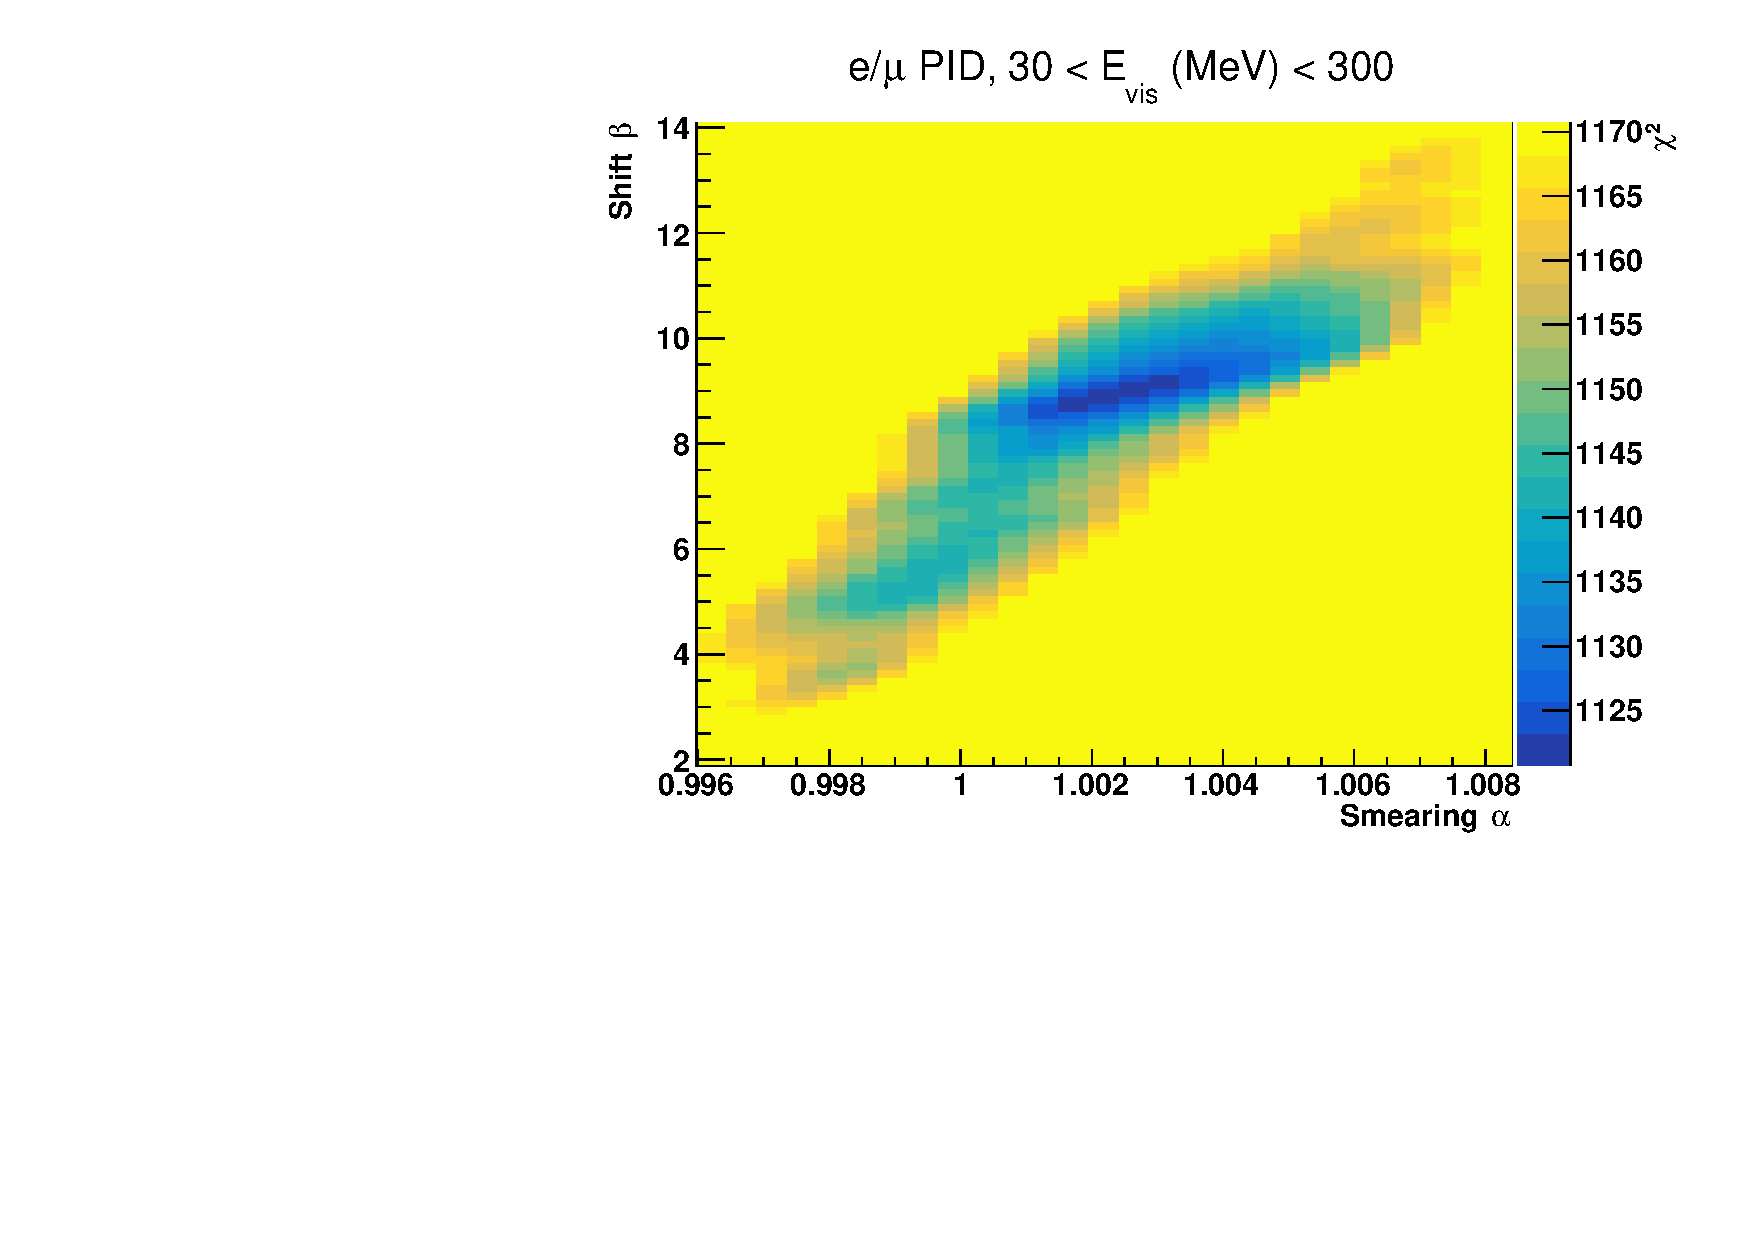
\includegraphics[width=\textwidth, trim={0mm 0mm 0mm 0mm}, clip,page=1]{Figures/Selections/EMUPID_Elt300_Chi2Map.pdf}
  \end{subfigure}%
  \begin{subfigure}[t]{0.49\textwidth}
    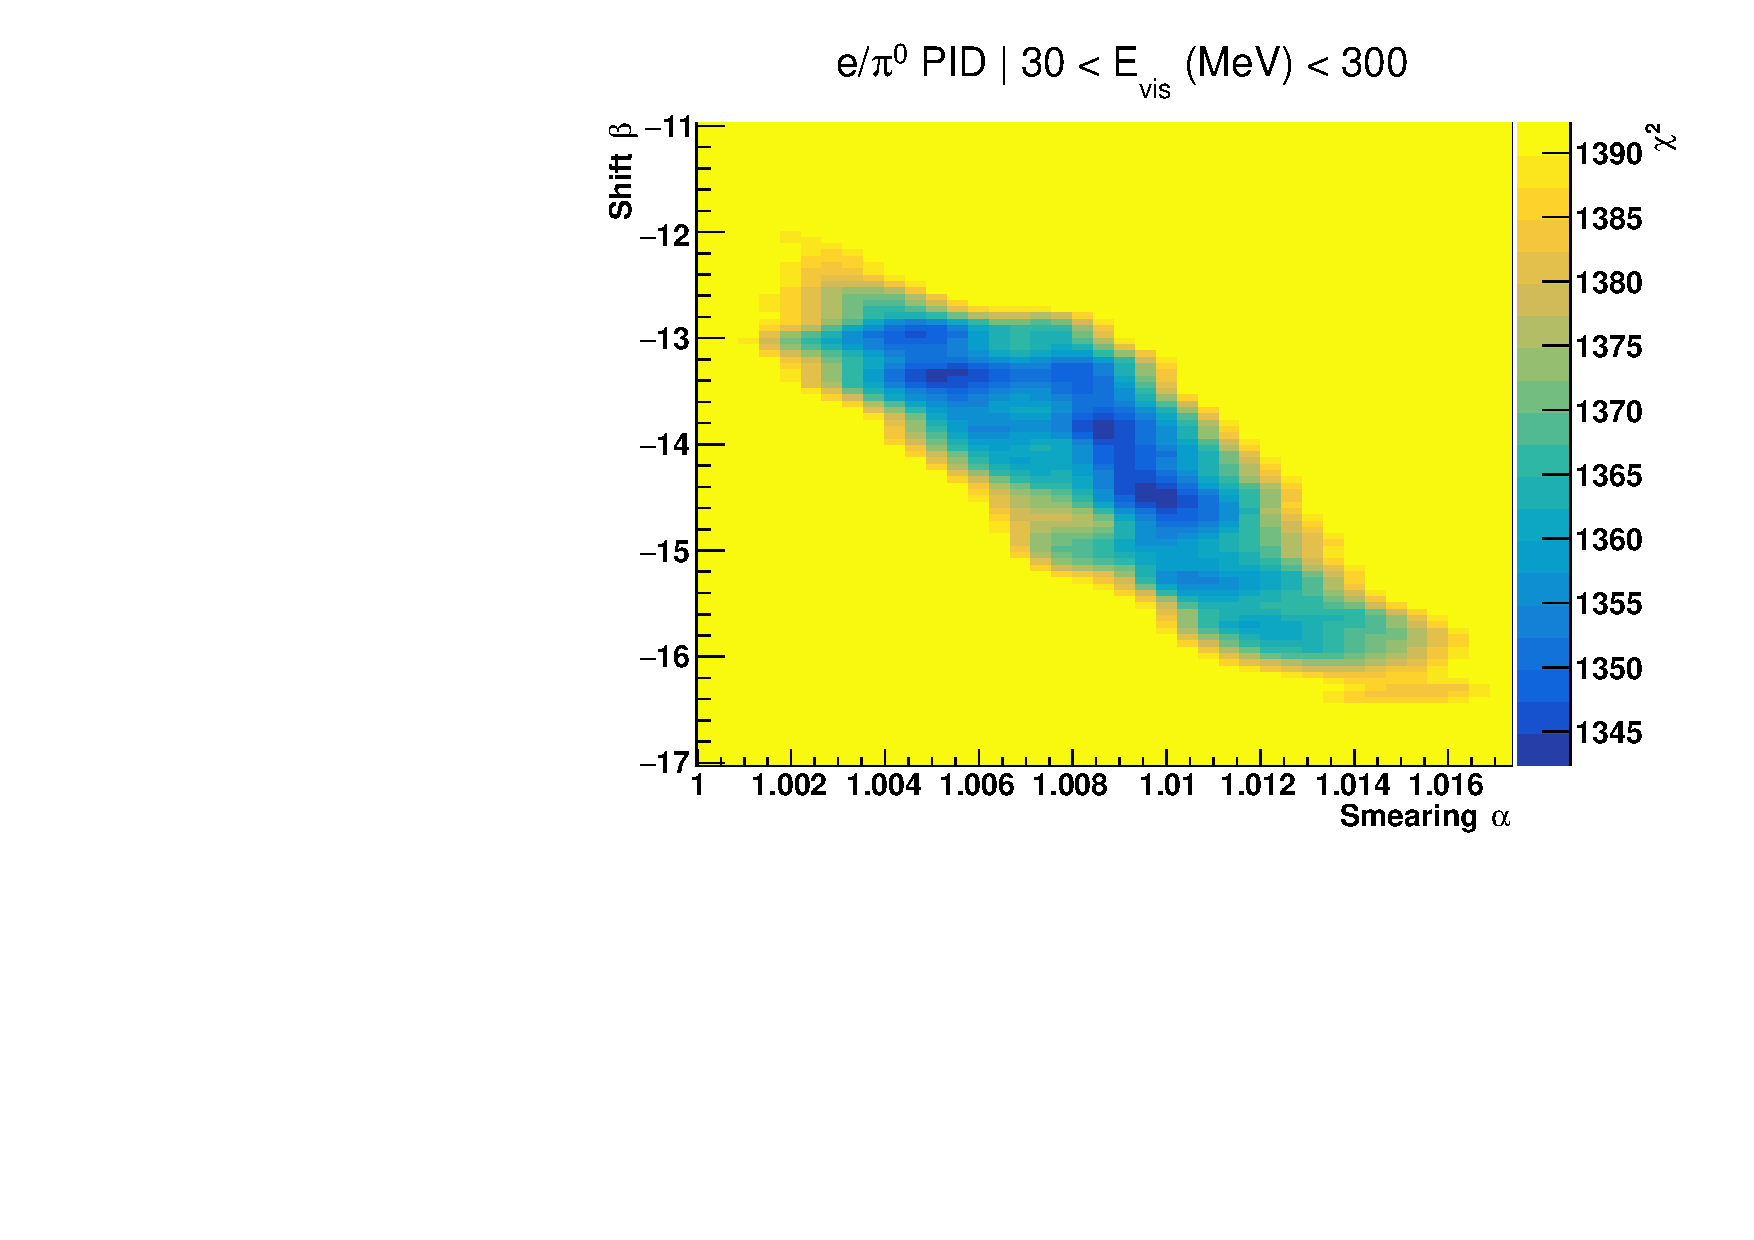
\includegraphics[width=\textwidth, trim={0mm 0mm 0mm 0mm}, clip,page=1]{Figures/Selections/EPI0PID_Elt300_Chi2Map.pdf}
  \end{subfigure}
  \caption{The \quickmath{\chi^{2}} between the hybrid-\quickmath{\pi^{0}} Monte Carlo and data samples, as a function of smear (\quickmath{\alpha}) and shift (\quickmath{\beta}) parameters, for events which have \quickmath{1\pi^{0}} final state topology. Left: Electron-muon separation PID parameter for events with \quickmath{30 \geq E_{vis} (MeV) < 300}. Right: Electron-\quickmath{\pi^{0}} separation PID parametter for events with \quickmath{30 \geq E_{vis} (MeV) < 300}.}
  \label{fig:SelsAndSysts_HybridChi2Maps}
\end{figure}

Similarly, the supplementary systematics which are added into the covariance from stopping muon and decay electron studies need to be included. A new framework \cite{t2ksk-common} was built in tandem with the T2K-SK working group \cite{t2k_tn_326} so the additional parameters can be incorporated into the MaCh3 framework. These are applied as normalisation parameters, depending on the particular interaction mode, number of tagged decay electrons, and whether the primary particle generated Cherenkov light. They are assigned Gaussian uncertainties with widths described by a covariance matrix.

Finally, the secondary interaction and photo-nuclear effects need to be accounted for in this detector model. In the T2K-only analysis, a covariance matrix was built to describe the response of the samples to variations of these parameters which was then added in quadrature to the detector covariance matrix. However, this technique can not be applied in the correlated detector model. Consequently, a binned response of each of the secondary interaction systematic parameters and the photo-nuclear response was generated and included through splined shape parameters, similar to the application of shape parameters in the cross-section model (see \autoref{sec:SelsAndSysts_Systs_Interaction}).

There are a total of \quickmath{224} \quickmath{\alpha^{i}_{jk}} and \quickmath{\beta^{i}_{jk}} parameters, of which \quickmath{32} have prior constraints from the hybrid \quickmath{\pi^0} samples.

One final complexity of this correlated detector model is that the two sets of samples, beam and subGeV atmospheric, use slightly different parameters to distinguish electron and muon-like events. The beam-only events use the \quickmath{\log(L_{e}/L_{\mu})} whereas the atmospheric samples use \quickmath{\log(L_{e}/L_{\pi})}, where \quickmath{L_{X}} is the likelihood for hypothesis \quickmath{X}. This is because the beam-only fits use single-ring \fq fitting techniques, whereas multi-ring fits are applied to the atmospheric samples where only the electron and pion hypothesis are considered. As discussed in \autoref{sec:Simulation_Reconstruction}, the pion hypothesis is a very good approximation of the muon hypothesis due to their similar mass. The correlation between the two likelihood ratios is illustrated in \autoref{fig:SelsAndSysts_LLHCorrelation}. A very strong correlation is clearly shown. Consequently, using the same shift and smear parameters correlated between the beam and subGeV atmospheric samples is a good approximation.

\begin{figure}[h]
  \begin{subfigure}[t]{0.49\textwidth}
    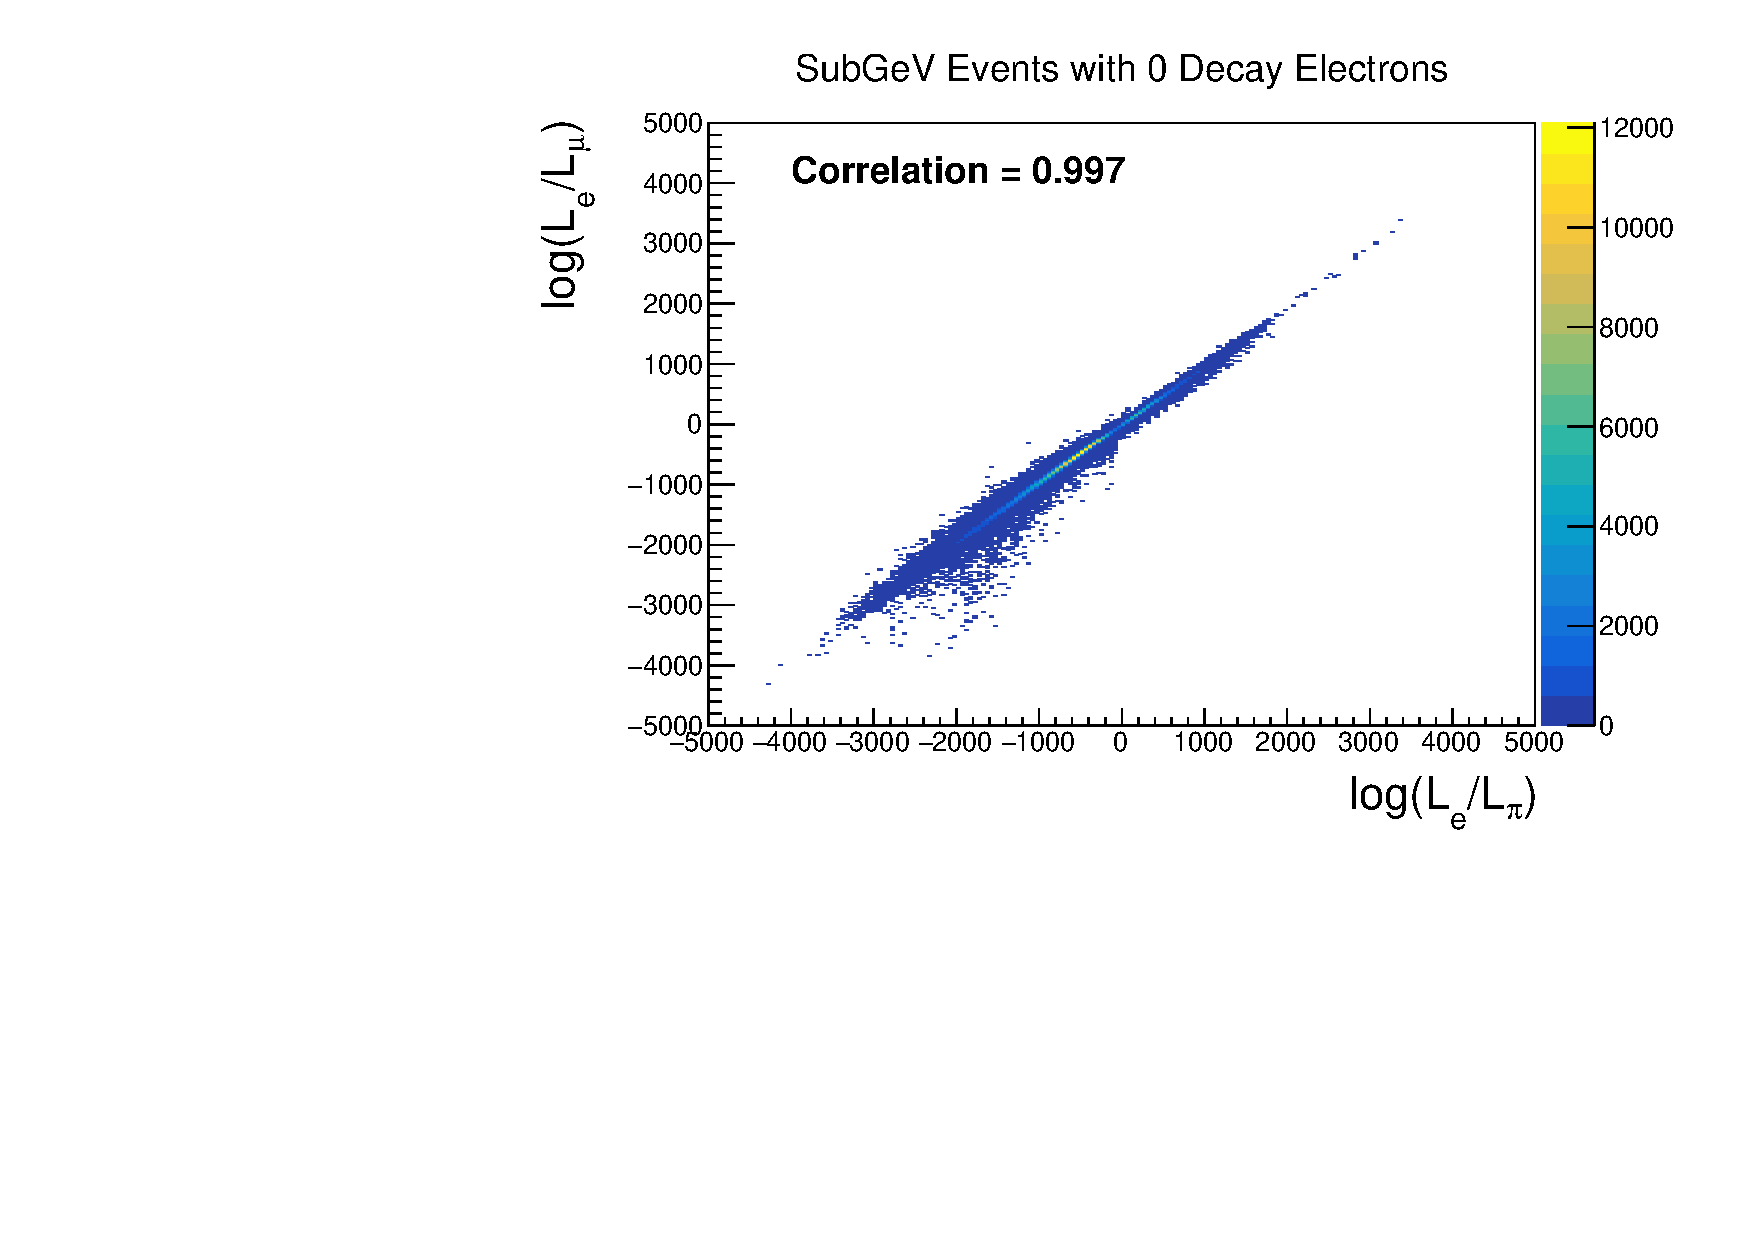
\includegraphics[width=\textwidth, trim={0mm 0mm 0mm 0mm}, clip,page=1]{Figures/Selections/Correlation_SG0Dcy.pdf}
  \end{subfigure}%
  \begin{subfigure}[t]{0.49\textwidth}
    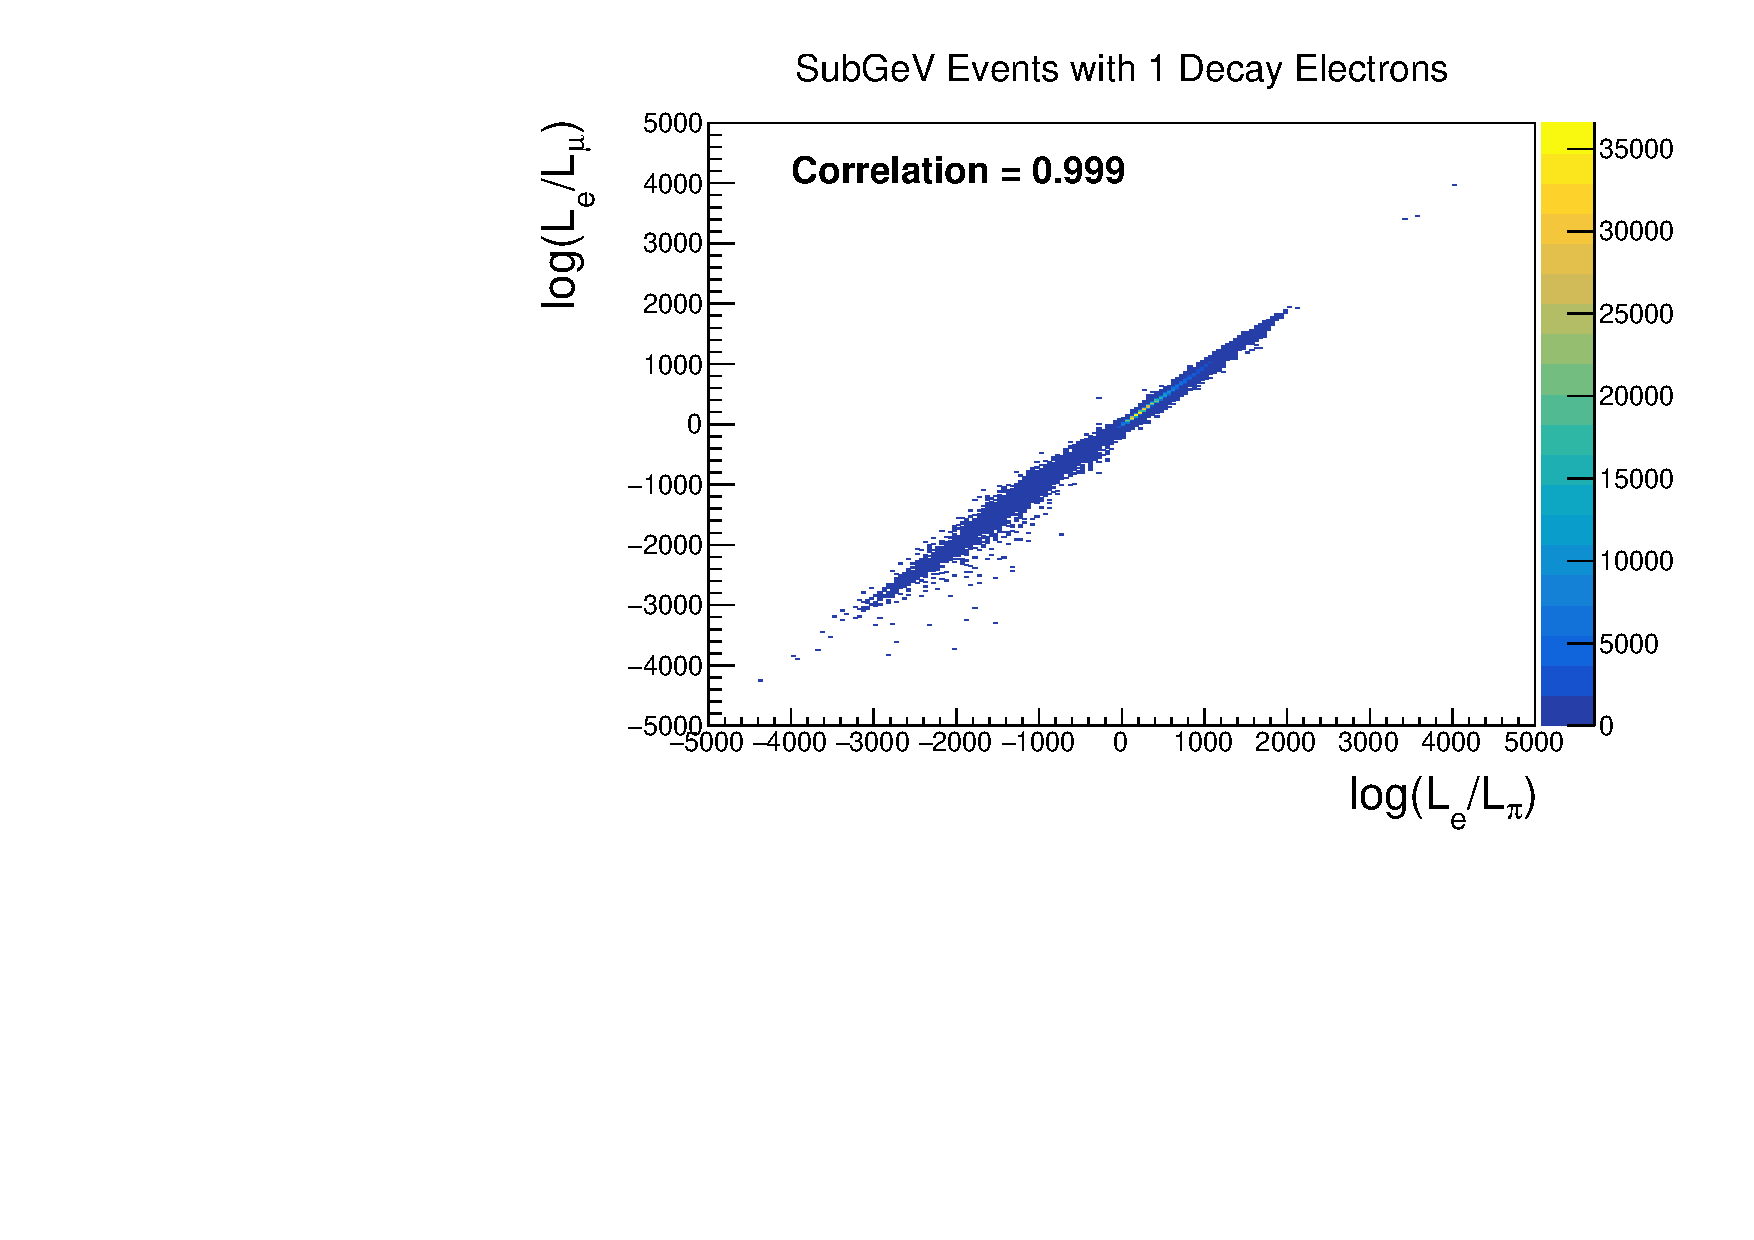
\includegraphics[width=\textwidth, trim={0mm 0mm 0mm 0mm}, clip,page=1]{Figures/Selections/Correlation_SG1Dcy.pdf}
  \end{subfigure}
  \begin{subfigure}[t]{0.49\textwidth}
    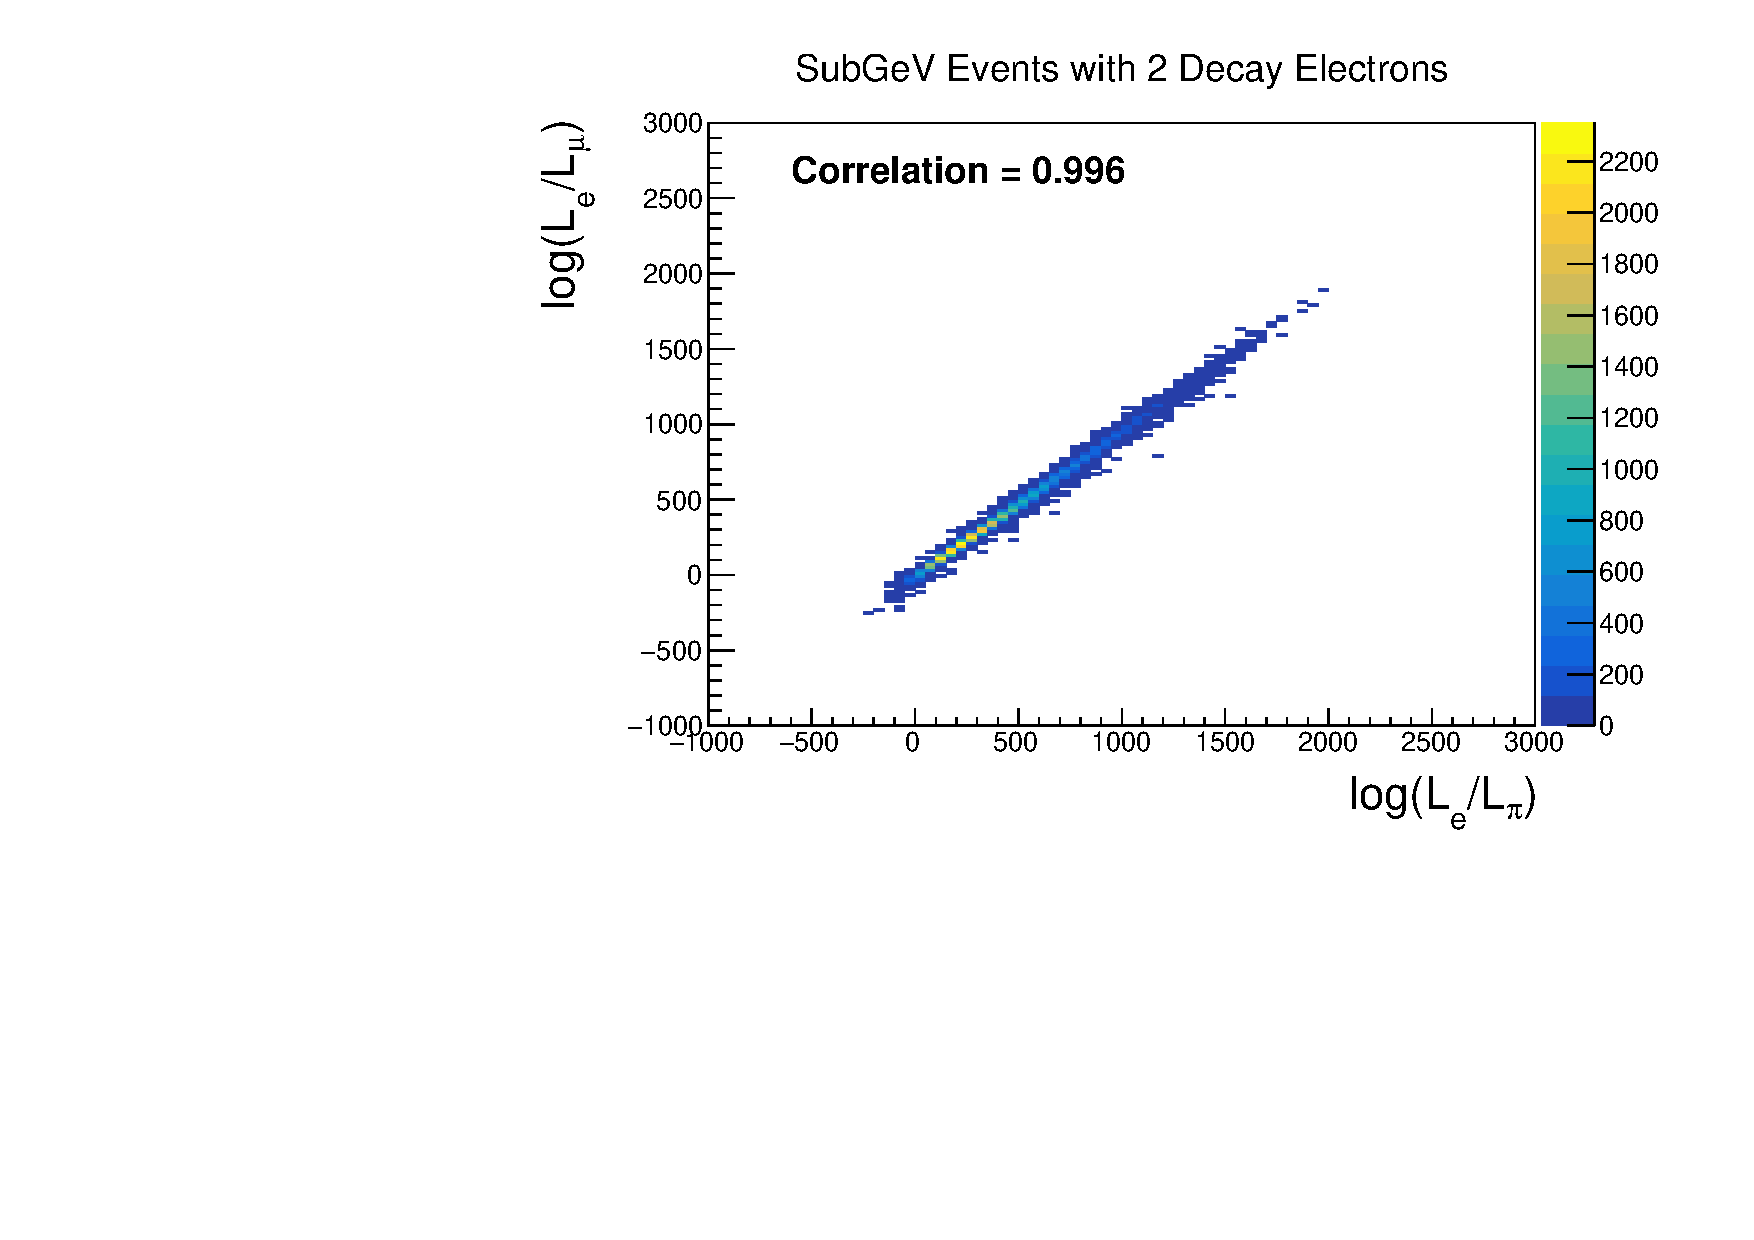
\includegraphics[width=\textwidth, trim={0mm 0mm 0mm 0mm}, clip,page=1]{Figures/Selections/Correlation_SG2Dcy.pdf}
  \end{subfigure}
  \caption{The distribution of \quickmath{\log(L_{e}/L_{\mu})} compared to \quickmath{\log(L_{e}/L_{\pi})} for subGeV events with zero (top left), one (top right) or two (bottom) decay electrons. The correlation in the distribution is calculated as \quickmath{0.997}, \quickmath{0.999} and \quickmath{0.996}, respectively.}
  \label{fig:SelsAndSysts_LLHCorrelation}
\end{figure}
